\documentclass[]{article}
\usepackage{lmodern}
\usepackage{amssymb,amsmath}
\usepackage{ifxetex,ifluatex}
\usepackage{fixltx2e} % provides \textsubscript
\ifnum 0\ifxetex 1\fi\ifluatex 1\fi=0 % if pdftex
  \usepackage[T1]{fontenc}
  \usepackage[utf8]{inputenc}
\else % if luatex or xelatex
  \ifxetex
    \usepackage{mathspec}
  \else
    \usepackage{fontspec}
  \fi
  \defaultfontfeatures{Ligatures=TeX,Scale=MatchLowercase}
\fi
% use upquote if available, for straight quotes in verbatim environments
\IfFileExists{upquote.sty}{\usepackage{upquote}}{}
% use microtype if available
\IfFileExists{microtype.sty}{%
\usepackage{microtype}
\UseMicrotypeSet[protrusion]{basicmath} % disable protrusion for tt fonts
}{}
\usepackage[margin=1in]{geometry}
\usepackage{hyperref}
\hypersetup{unicode=true,
            pdftitle={Comparação de métodos de imputação de dados ausentes sob diferentes mecanismos},
            pdfborder={0 0 0},
            breaklinks=true}
\urlstyle{same}  % don't use monospace font for urls
\usepackage{graphicx,grffile}
\makeatletter
\def\maxwidth{\ifdim\Gin@nat@width>\linewidth\linewidth\else\Gin@nat@width\fi}
\def\maxheight{\ifdim\Gin@nat@height>\textheight\textheight\else\Gin@nat@height\fi}
\makeatother
% Scale images if necessary, so that they will not overflow the page
% margins by default, and it is still possible to overwrite the defaults
% using explicit options in \includegraphics[width, height, ...]{}
\setkeys{Gin}{width=\maxwidth,height=\maxheight,keepaspectratio}
\IfFileExists{parskip.sty}{%
\usepackage{parskip}
}{% else
\setlength{\parindent}{0pt}
\setlength{\parskip}{6pt plus 2pt minus 1pt}
}
\setlength{\emergencystretch}{3em}  % prevent overfull lines
\providecommand{\tightlist}{%
  \setlength{\itemsep}{0pt}\setlength{\parskip}{0pt}}
\setcounter{secnumdepth}{5}
% Redefines (sub)paragraphs to behave more like sections
\ifx\paragraph\undefined\else
\let\oldparagraph\paragraph
\renewcommand{\paragraph}[1]{\oldparagraph{#1}\mbox{}}
\fi
\ifx\subparagraph\undefined\else
\let\oldsubparagraph\subparagraph
\renewcommand{\subparagraph}[1]{\oldsubparagraph{#1}\mbox{}}
\fi

%%% Use protect on footnotes to avoid problems with footnotes in titles
\let\rmarkdownfootnote\footnote%
\def\footnote{\protect\rmarkdownfootnote}

%%% Change title format to be more compact
\usepackage{titling}

% Create subtitle command for use in maketitle
\newcommand{\subtitle}[1]{
  \posttitle{
    \begin{center}\large#1\end{center}
    }
}

\setlength{\droptitle}{-2em}

  \title{Comparação de métodos de imputação de dados ausentes sob diferentes
mecanismos}
    \pretitle{\vspace{\droptitle}\centering\huge}
  \posttitle{\par}
    \author{Fernanda Buzza Alves Barros\textsuperscript{1}, Thaís
Paiva\textsuperscript{2}\\
1. Aluna\\
2. Orientadora}
    \preauthor{\centering\large\emph}
  \postauthor{\par}
      \predate{\centering\large\emph}
  \postdate{\par}
    \date{28 de fevereiro de 2019}

\usepackage{float}

\begin{document}
\maketitle

\section{INTRODUÇÃO}\label{introducao}

Problemas de dados faltantes em bancos de dados são recorrentes, e
interferem diretamente nas inferências e tomada de decisões decorrentes
do estudo do banco de dados. Um exemplo seriam perguntas constrangedoras
como o consumo de drogas ilícitas, infração de leis de trânsito e
doenças sexualmente transmissíveis.

Assim temos a principal questão: como inferir informações dos valores
ausentes? Vários métodos foram propostos para solucionar este problema
como a Análise de Casos Completos (ACC) e Imputação Múltipla, sendo a
última o foco dessa pesquisa. Essa abordagem, prosposta por Little e
Rubin (1987) e aprimorada por outros pesquisadores como Schafer (1997) e
Van Buuren e Groothuis-Oudshoorn (2011), consiste em preencher os dados
faltantes aleatoriamente com valores candidatos baseados nos valores
observados.

\section{METODOLOGIA}\label{metodologia}

Para esse estudo aplicamos a metodologia de três diferentes mecanismos
de geração de dados ausentes Perda Completamente Aleatória (PCA), Perda
Aleatória (PA) e Perda Não Aleatória (PNA). Na PCA o motivo pelo qual os
dados estão ausentes não está relacionado às variáveis do estudo; já na
PA a razão para um valor estar ausente está relacionada às outras
variáveis observadas, mas não está relacionada à variável em que há
valores ausentes; e por fim na PNA o motivo pelo qual os dados estão
ausentes está diretamente relacionado aos valores não observados da
variável de interesse.

Após gerar os dados ausentes aplicamos a metodologia da Imputação
Múltipla, que consiste em gerar valores (m vezes) para os dados
faltantes, sendo que ela cria uma matriz com todas as M imputações. Para
realização das imputações utilizamos o pacote \emph{Multivariate
Imputation With Chained Equations (MICE)} Van Buuren, S.,
Groothuis-Oudshoorn, K. (2011). A função que realiza a imputação
chama-se \emph{mice}, e nesse estudo realizamos a imputação 5 vezes
(m=5). A aplicação dessa função requer um método que varia de acordo com
o tipo de escala da variável de interesse numérico, fator, fator de dois
níveis, fator acima de 2 níveis e qualquer tipo de escala. Para os tipos
de escala númericos existem os seguintes métodos: \emph{Predictive mean
matching (pmm)}, \emph{Bayesian linear regression (norm)}, \emph{Linear
regression, non-Bayesian (norm.nob)}, \emph{Unconditional mean
imputation (mean)} e \emph{Two-level linear model (2l.norm)}. Já para os
tipos de escala fator existem os seguintes métodos: \emph{Logistic
regression (logreg)}, \emph{Polytomous (unordered) regression (polyreg)}
e \emph{Linear discriminant analysis (lda)}. E por fim para qualquer
tipo de escala existe o método \emph{Random sample from the observed
data (sample)}.

Como a variável de interesse desse estudo é numérica, optamos por um
método em que o tipo de escala é numérico, assim o método escolhido foi
o \emph{Predictive mean matching (pmm)}.

\subsection{Predictive mean matching
(pmm)}\label{predictive-mean-matching-pmm}

O método da \emph{pmm} consiste em escolher valores possíveis para as
observações faltantes baseando-se nas observações que possuem valores
completos. A escolha dos valores variam entre 3, 5 ou 10 possíveis
candidatos com valores completos, que são chamados de doadores.

Os doadores são escolhidos aleatoriamente e assumindo que a distribuição
das observações com valores ausentes segue a mesma distribuição das
observações com valores completos.

O método é bastante robusto para transformações da variável de
interesse, que será o caso nessa pesquisa, e também é válido para
variáveis discretas presentes no banco de dados. Como o método é baseado
nas observações completas, os valores gerados são bastante realistas e
não serão imputados valores fora da amplitude dos dados.

\section{RESULTADOS}\label{resultados}

\subsection{Banco de dados}\label{banco-de-dados}

Para realizar a imputação dos dados utilizamos o banco de dados \emph{US
Term Life insurance} do pacote \emph{CASdatasets} disponível no software
estatístico R. O banco de dados é uma amostra de 500 domicílios retirada
da pesquisa de finanças de consumidores (Survey of Consumer Finances),
realizada em 2004 nos Estados Unidos da América (EUA). As imputações e
os resultados foram obtidos utilizando esse mesmo software estatístico.
O banco de dados possui 18 variáveis com 500 observações, como pode ser
visto abaixo.

\begin{verbatim}
## 'data.frame':    500 obs. of  18 variables:
##  $ Gender         : int  1 1 1 1 1 1 0 1 1 1 ...
##  $ Age            : int  30 50 39 43 61 34 75 29 35 70 ...
##  $ MarStat        : int  1 1 1 1 1 2 0 1 2 1 ...
##  $ Education      : int  16 9 16 17 15 11 8 16 4 17 ...
##  $ Ethnicity      : int  3 3 1 1 1 2 1 1 3 1 ...
##  $ SmarStat       : int  2 1 2 1 2 1 0 2 1 2 ...
##  $ Sgender        : int  2 2 2 2 2 2 0 2 2 2 ...
##  $ Sage           : int  27 47 38 35 59 31 0 31 45 74 ...
##  $ Seducation     : int  16 8 16 14 12 14 0 17 9 16 ...
##  $ NumHH          : int  3 3 5 4 2 4 1 3 2 2 ...
##  $ Income         : int  43000 12000 120000 40000 25000 28000 2500 100000 20000 101000 ...
##  $ TotIncome      : int  43000 0 90000 40000 1020000 0 0 84000 0 6510000 ...
##  $ Charity        : int  0 0 500 0 500 0 0 0 0 284000 ...
##  $ Face           : int  20000 130000 1500000 50000 0 220000 0 600000 0 0 ...
##  $ FaceCVLifePol  : int  0 0 0 75000 7000000 0 14000 0 0 2350000 ...
##  $ CashCVLifePol  : int  0 0 0 0 300000 0 5000 0 0 0 ...
##  $ BorrowCVLifePol: int  0 0 0 5 5 0 5 0 0 5 ...
##  $ NetValue       : int  0 0 0 0 0 0 0 0 0 0 ...
\end{verbatim}

Selecionamos as seguintes variáveis para realizar a pesquisa: Gênero
(gênero do entrevistado); Idade (idade do entrevistado); Estado Civil
(estado civil do entrevistado); Escolaridade (número de anos de
escolaridade do entrevistado); Etnia (etnia do entrevistado); Renda
(renda anual da família do entrevistado).

Primeiras observações do banco de dados original:

\begin{verbatim}
##      Gender Age        MarStat Education  Ethnicity Income
## 1 Masculino  30         Casado        16 Hispânico  43000
## 2 Masculino  50         Casado         9 Hispânico  12000
## 3 Masculino  39         Casado        16     Branco 120000
## 4 Masculino  43         Casado        17     Branco  40000
## 5 Masculino  61         Casado        15     Branco  25000
## 6 Masculino  34 Morando Juntos        11      Negro  28000
##           Education2
## 1    Ensino Superior
## 2 Ensino Fundamental
## 3    Ensino Superior
## 4    Ensino Superior
## 5    Ensino Superior
## 6      Ensino Médio
\end{verbatim}

\subsection{Análise Descritiva}\label{analise-descritiva}

Após a escolha das variáveis para esse estudo, iremos realizar uma
análise descritiva de cada uma delas, e assim avaliar as relações
existentes entre a variável resposta e as covariáveis do banco de dados.
Ao final realizaremos um dos principais objetivos dessa pesquisa, que é
verificar os possíveis questionamentos sobre a Renda a partir das outras
variáveis.

Primeiramente analisaremos as variáveis individualmente, com interesse
em suas distribuições e comportamentos. Pelos dados observamos que as
variáveis contínuas são: Renda, Idade e Escolaridade, e as variáveis
discretas são: Gênero, Estado Civil e Etnia.

\begin{figure}[H]

{\centering 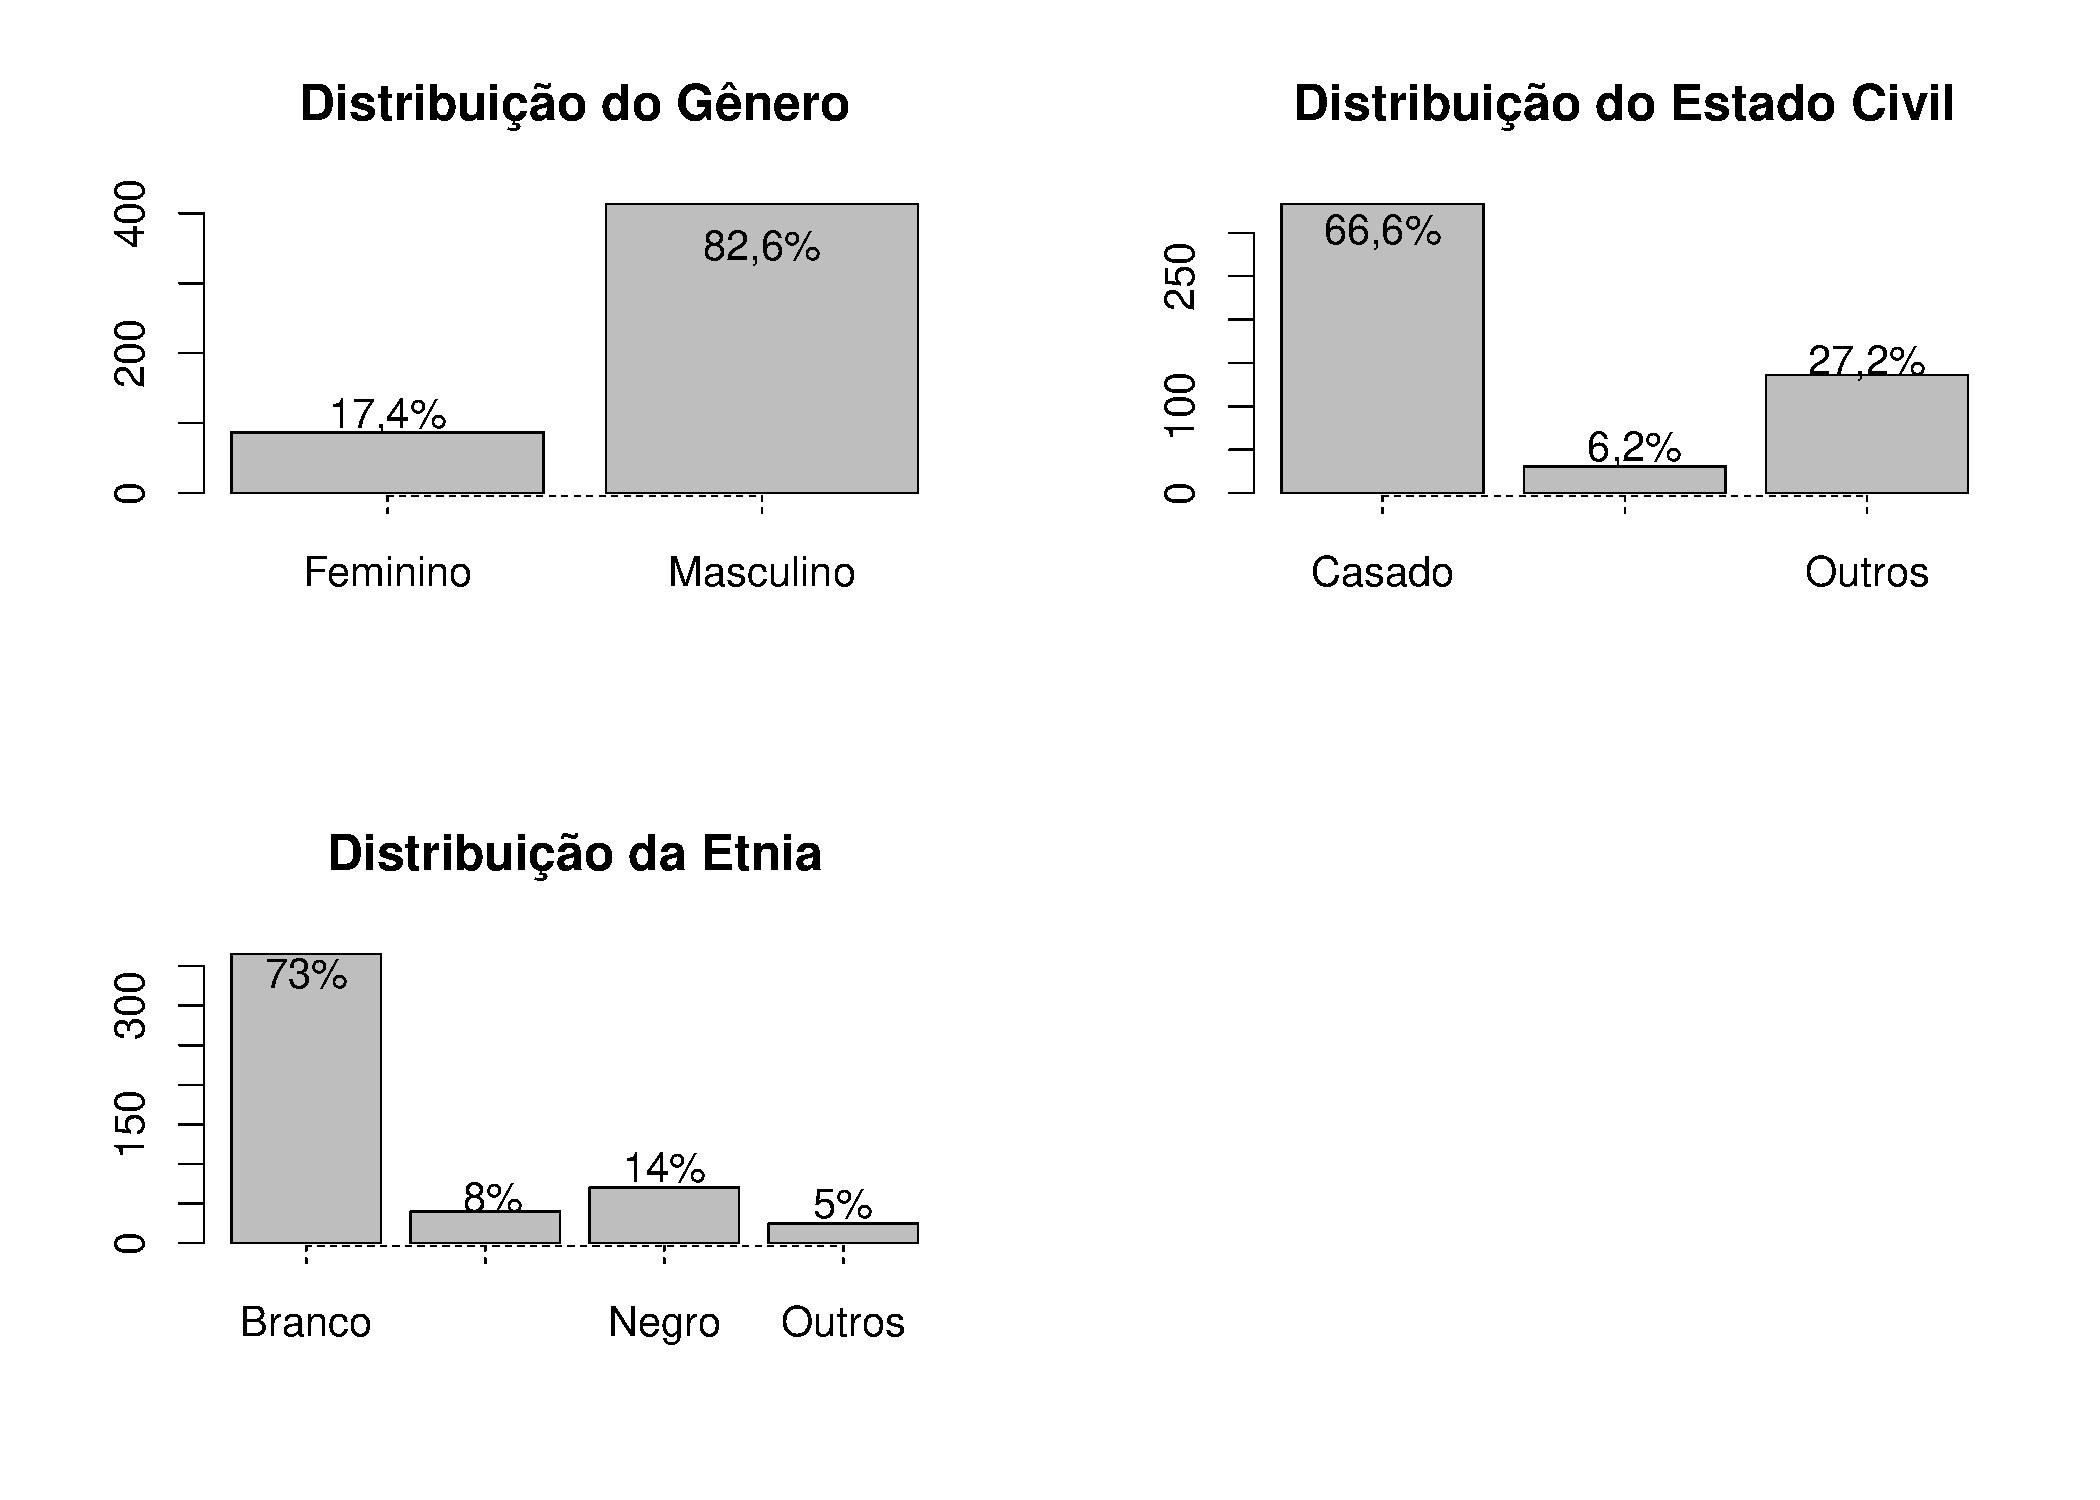
\includegraphics[width=1\linewidth]{p100-graf} 

}

\caption{Distribuição das variáveis discretas.}\label{fig:unnamed-chunk-6}
\end{figure}

Para as variáveis discretas temos que o banco de dados possui uma
quantidade maior de entrevistados do sexo masculino (413 entrevistados)
do que do sexo feminino (87 entrevistadas); para o estado civil temos
uma concentração maior de respostas para os entrevistados Casados (333
entrevistados) e a menor quantidade de entrevistados pertence ao estado
civil de Morando Juntos (31 entrevistados), sendo que o estado civil
Outros possui 136 entrevistados; por fim para a etnia temos uma maior
quantidade de entrevistados que possuem etnia Branco (365
entrevistados), sendo que as outras etnias possuem valores menores de
entrevistados no banco de dados: Hispânico (40 entrevistados), Negro (70
entrevistados) e Outros (25 entrevistados).

\begin{figure}[H]

{\centering 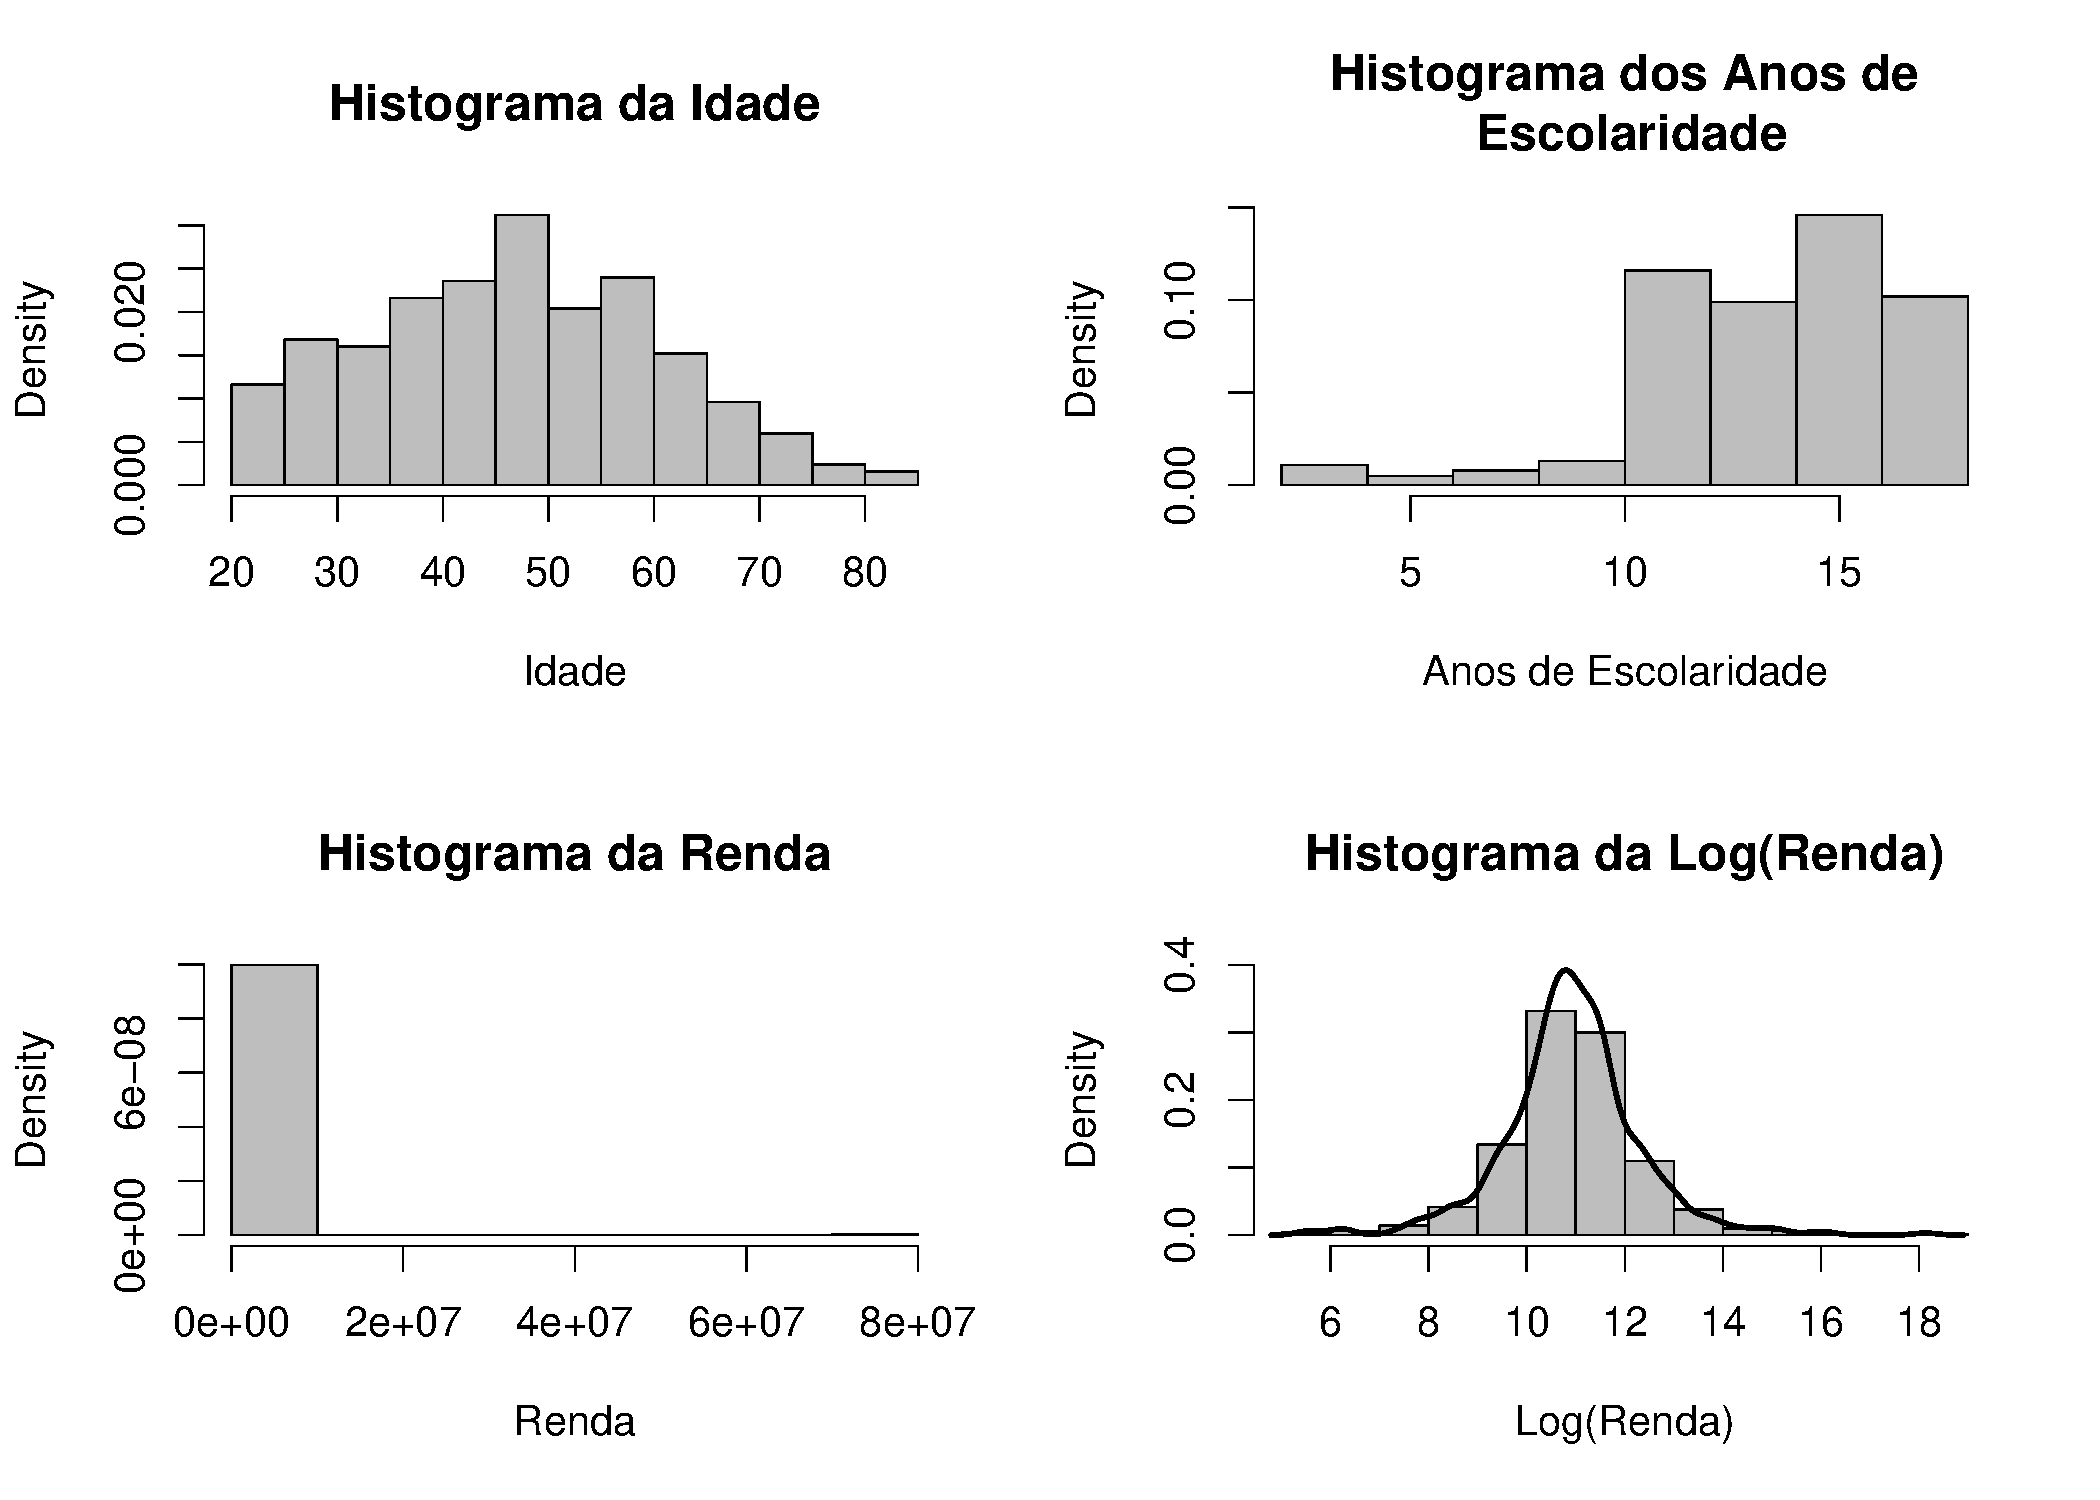
\includegraphics[width=0.6\linewidth]{p101-graf} 

}

\caption{Distribuição das variáveis contínuas.}\label{fig:unnamed-chunk-7}
\end{figure}

Para as variáveis contínuas temos que a variável Idade está na maior
parte distribuída entre os 20 anos e 70 anos, após 70 anos vemos poucos
entrevistados no banco de dados, sendo também que a idade máxima é 85
anos e a idade mínima é 20 anos. A média é 47.164 anos e a mediana 47
anos. O primeiro quantil é de 37 anos, representando a idade que deixa
25\% das observações abaixo e 75\% acima dessa idade. E o terceiro
quantil é de 58 anos, representando a idade que possui 75\% das
observações abaixo dela e 25\% das observações acima dela.

A distribuição da variável Escolaridade possui maior concentração de
entrevistados após 10 anos de escolaridade.

E para a variável Renda temos que a renda mínima anual é 260 dólares e a
renda máxima anual é 75000000 dólares. A mediana e a média são 54000
dólares e 321021 doláres, respectivamente. O primeiro quantil é de 28000
dólares, representando o valor de renda anual que deixa 25\% das
observações abaixo dela e 75\% acima dela. E o terceiro quantil é de
106000 dólares, representando a renda anual que possui 75\% das
observações abaixo dela e 25\% das observações acima dela. Aplicamos o
logarítimo para melhor visualização da distribuição da renda anual
através do histograma e percebemos uma aparência com a distribuição
normal.

Além da análise da variável Escolaridade em anos, foi realizada também a
análise dos anos de escolaridade divididos pelos tipos de ensino
existentes, que são: 2-10 anos de escolaridade corresponde ao Ensino
Fundamental, 11-14 anos de escolaridade corresponde ao Ensino Médio e de
15-17 anos de escolaridade corresponde ao Ensino Superior. Assim obtemos
a Figura 3:

\begin{figure}[H]

{\centering 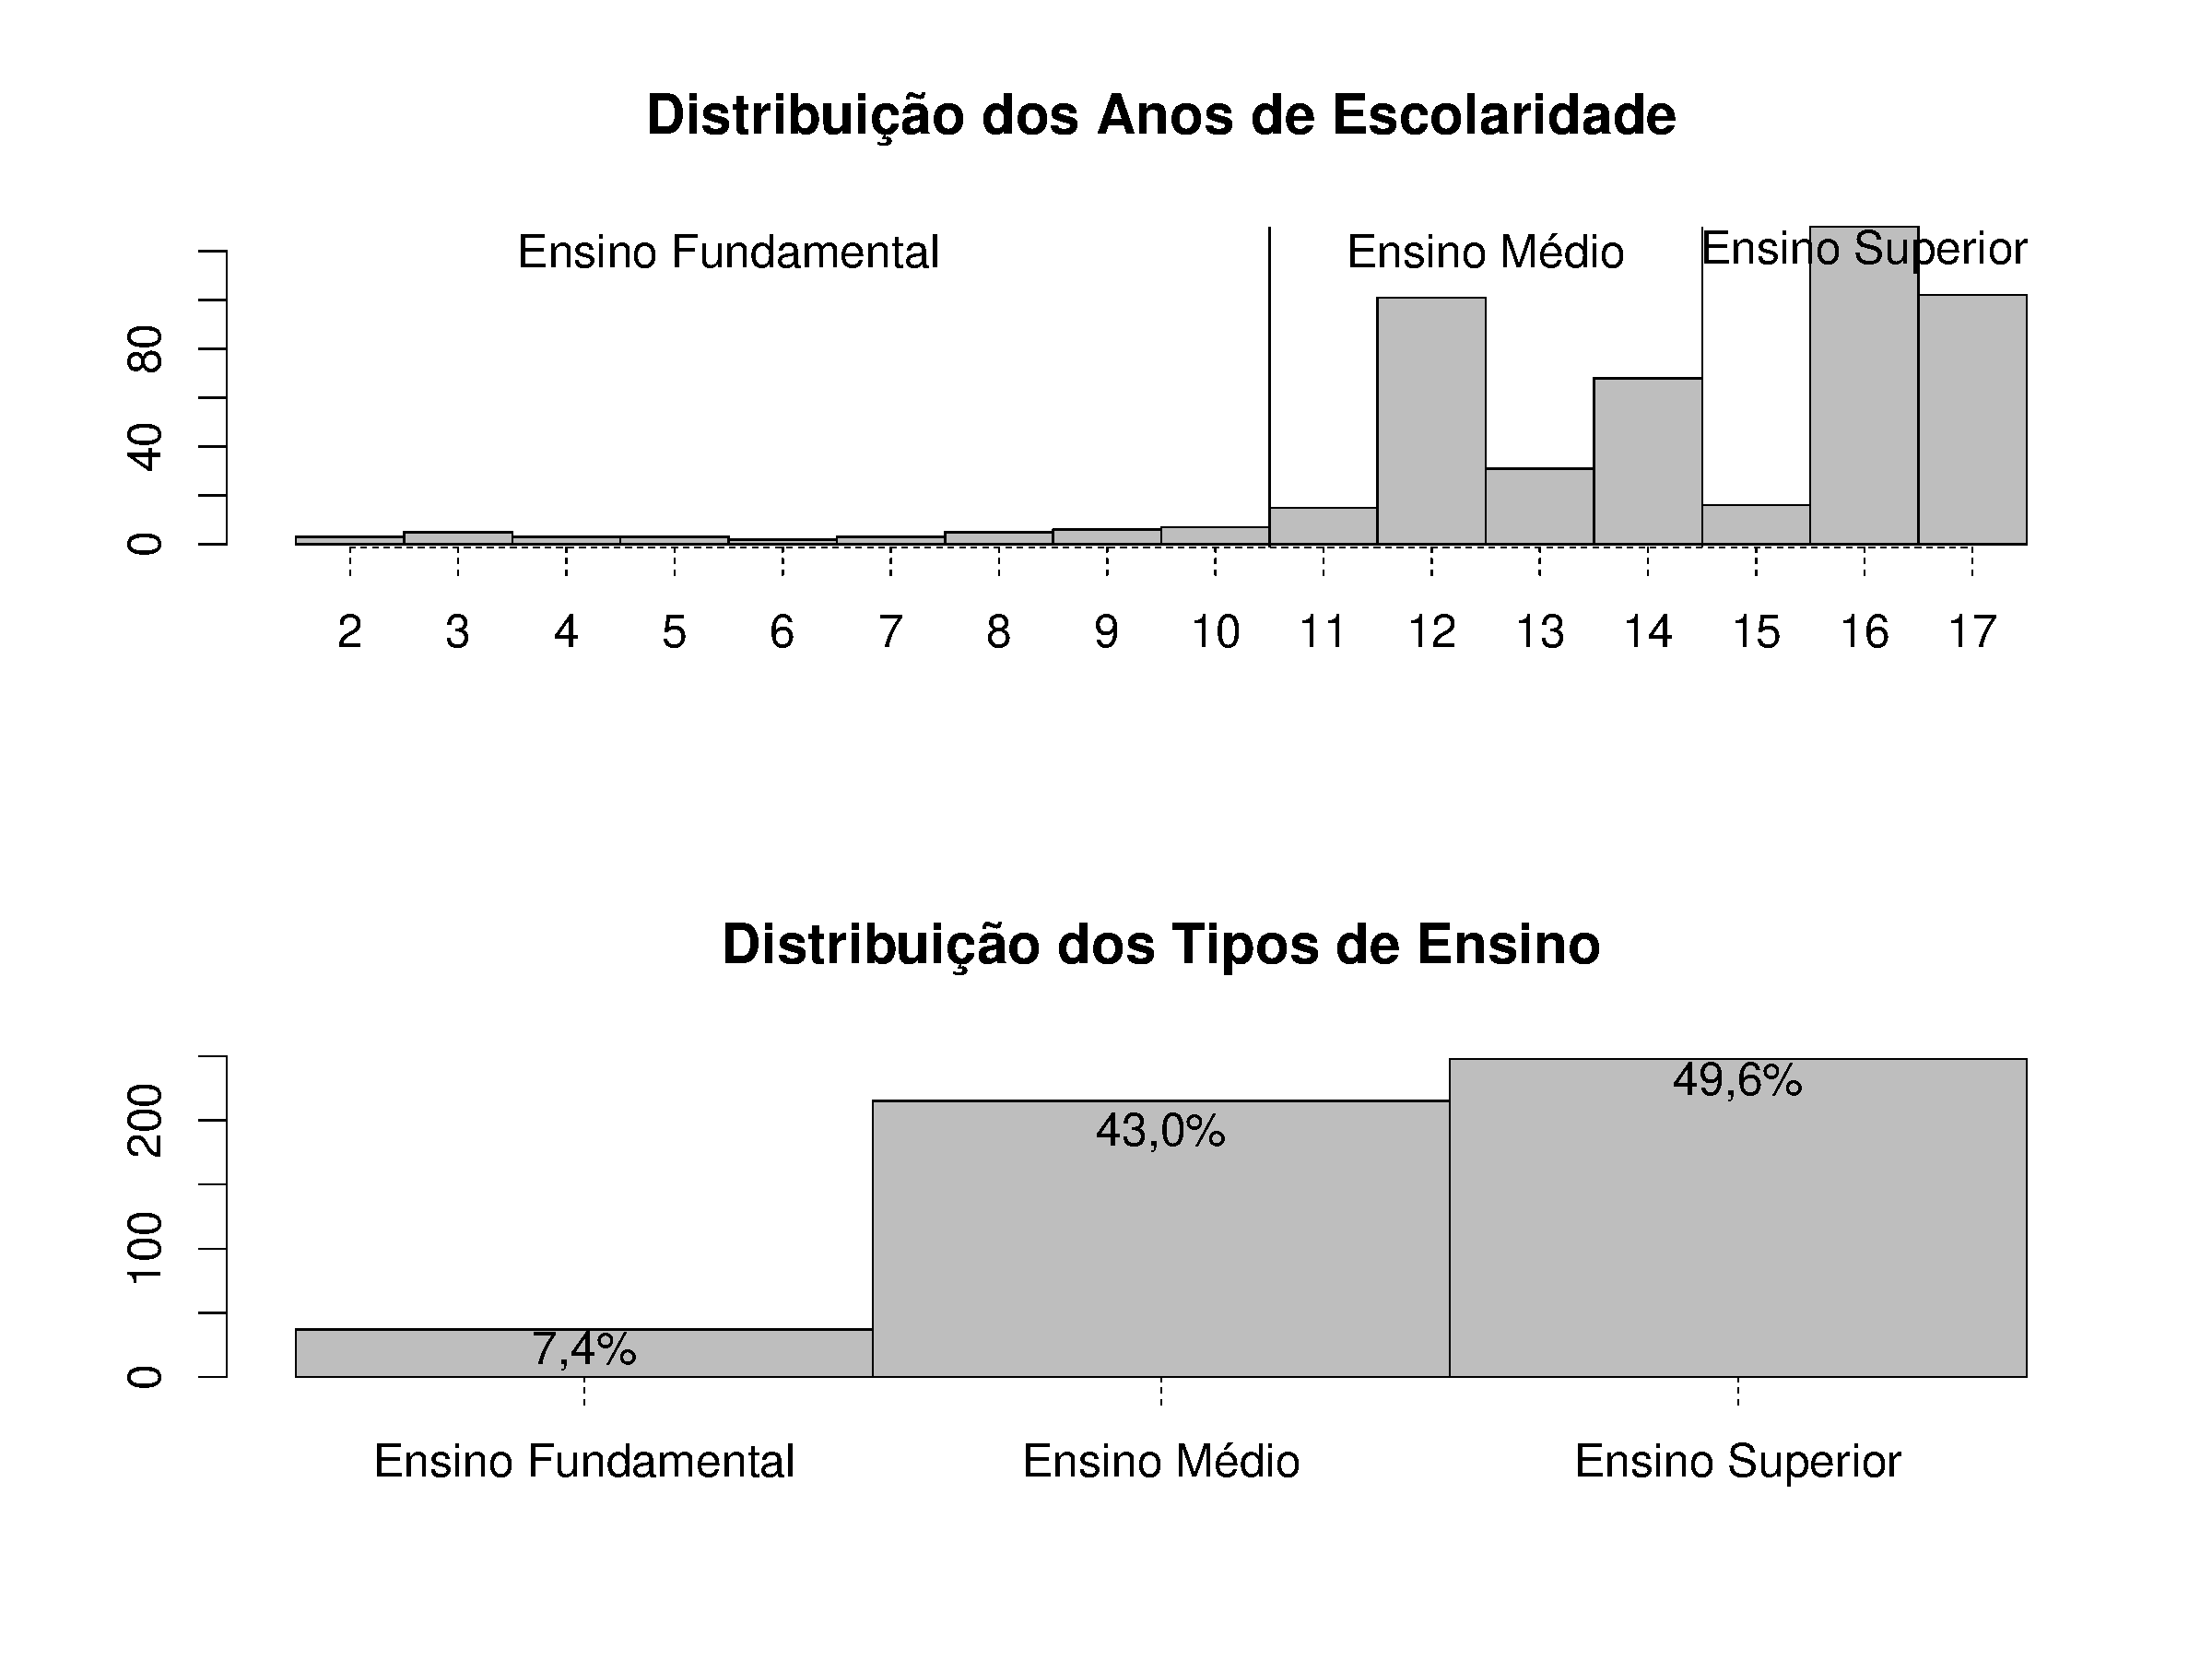
\includegraphics[width=0.6\linewidth]{p102-graf} 

}

\caption{Distribuição da escolaridade.}\label{fig:unnamed-chunk-10}
\end{figure}

Avaliando os tipos de ensino percebemos uma maior concentração de
entrevistados que possuem o ensino médio e o ensino superior, sendo que
quase a metade dos entrevistados possuem ensino superior, esse valor
corresponde a 248 entrevistados.

Analisamos também a relação entre a variável resposta (Renda) e as
covariáveis presentes no banco de dados escolhido. Assim obtivemos os
seguintes resultados:

\begin{figure}[H]

{\centering 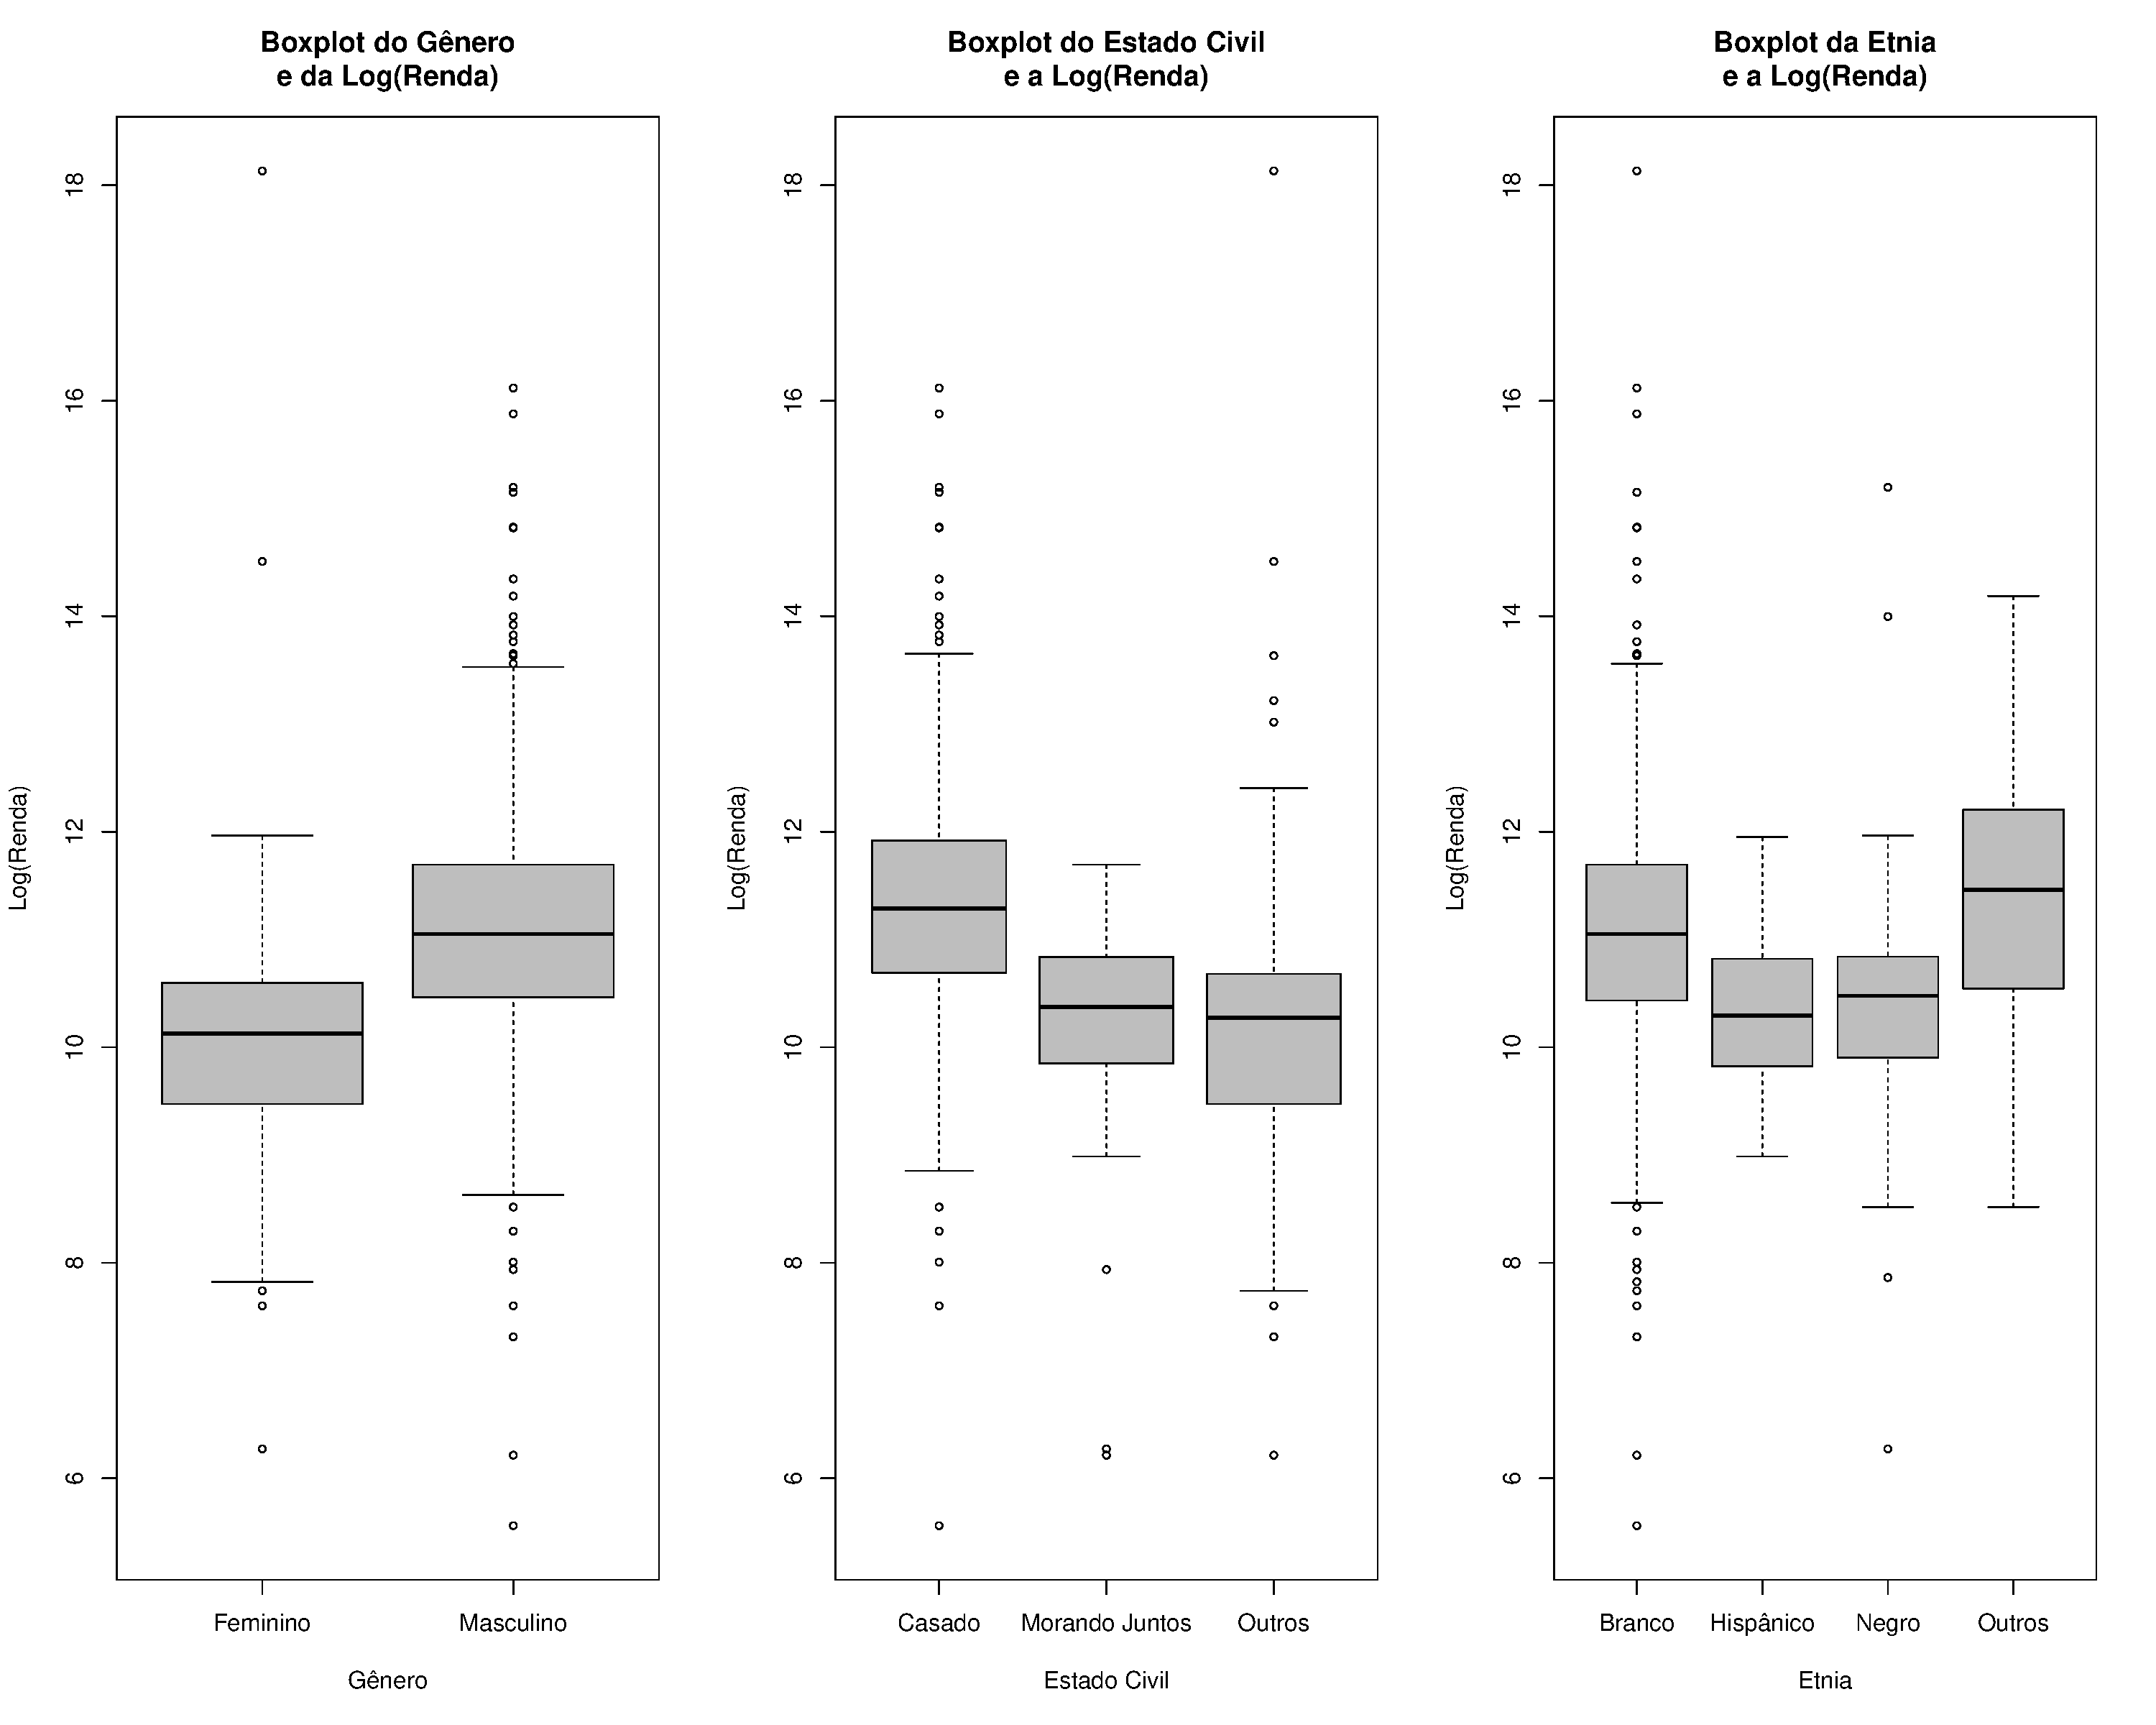
\includegraphics[width=0.8\linewidth]{p103-graf} 

}

\caption{Box-plots da Log(Renda) com as variáveis Gênero, Estado Civil e Etnia.}\label{fig:unnamed-chunk-11}
\end{figure}

Para as variáveis discretas temos os boxplots da Log(Renda) com cada uma
das variáveis separadamente. Para o gênero observamos um valor de renda
maior para o sexo masculino, comparando com o sexo feminino; já a
variável Estado Civil os entrevistados casados possuem uma renda maior,
sendo que a mediana da renda dos que moram juntos com o parceiro(a) e
outros estão bastante próximas, porém são inferiores aos valores de
renda dos entrevistados casados. Na comparação entre a Log(Renda) e a
Etnia percebemos uma amplitude da renda maior para as etnias Branco e
Outros, entretanto, como foi observado anteriormente, essas etnias
correspondem a 73\% e 5\%, respectivamente, do total do banco de dados.

\begin{figure}[H]

{\centering 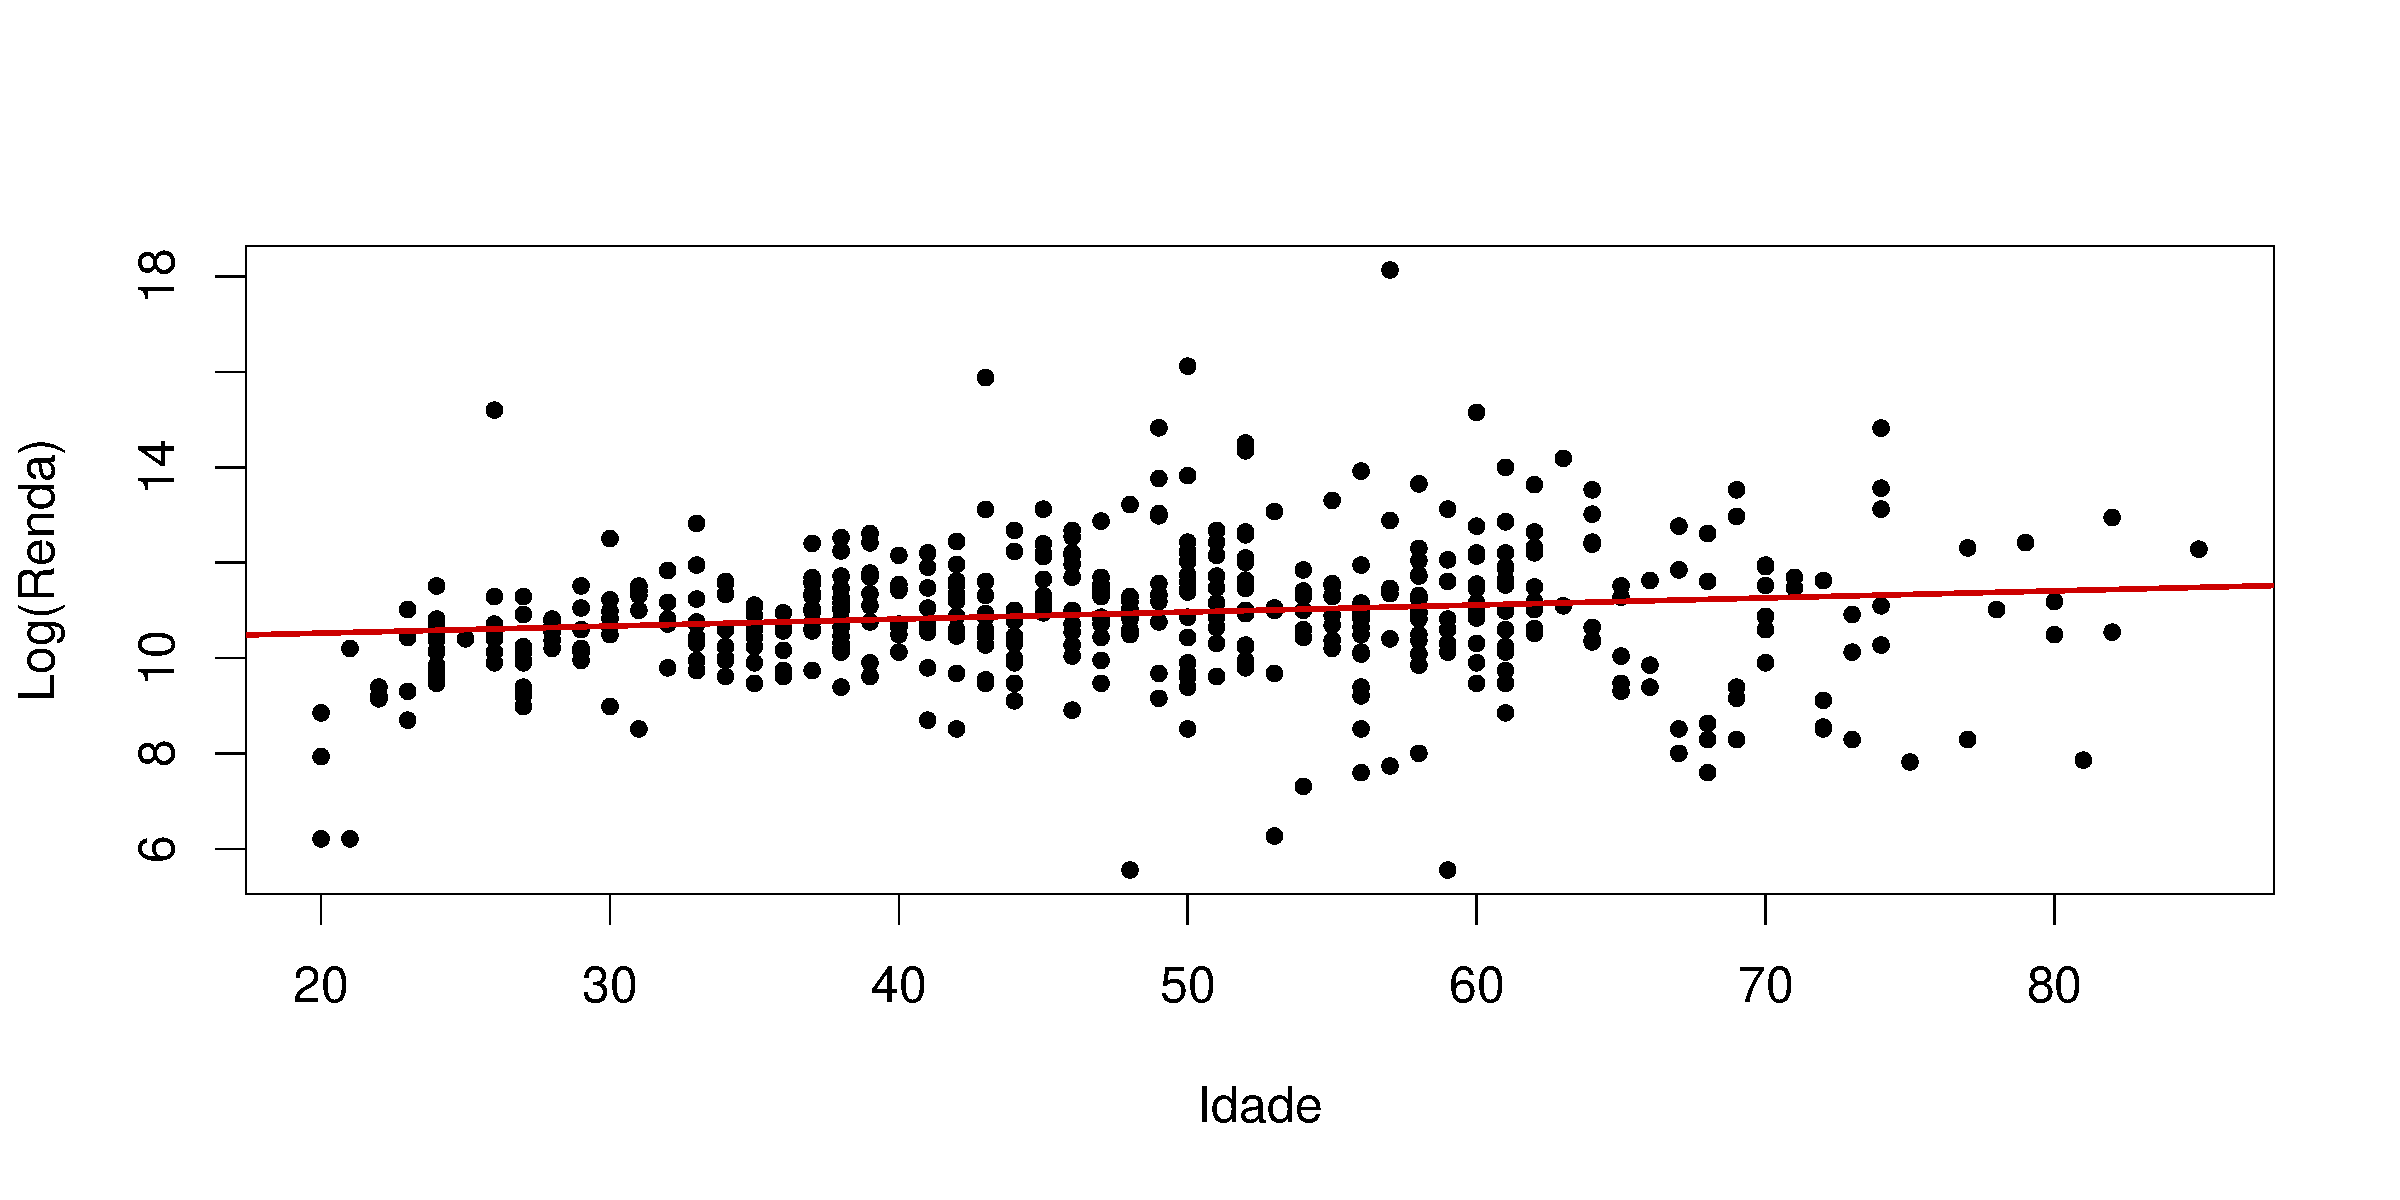
\includegraphics[width=0.6\linewidth]{p12-graf} 

}

\caption{Distribuição da Log(Renda) pela Idade.}\label{fig:unnamed-chunk-12}
\end{figure}

Para a relação entre as variáveis Log(Renda) e a Idade temos o gráfico
de dispersão da Figura 5, nele percebemos uma pequena inclinação no
ajuste da curva quando ocorre o aumento das idades dos entrevistados, o
que indica um possível ganho de renda anual maior para os entrevistados
a medida que aumenta a idade.

\begin{figure}[H]

{\centering 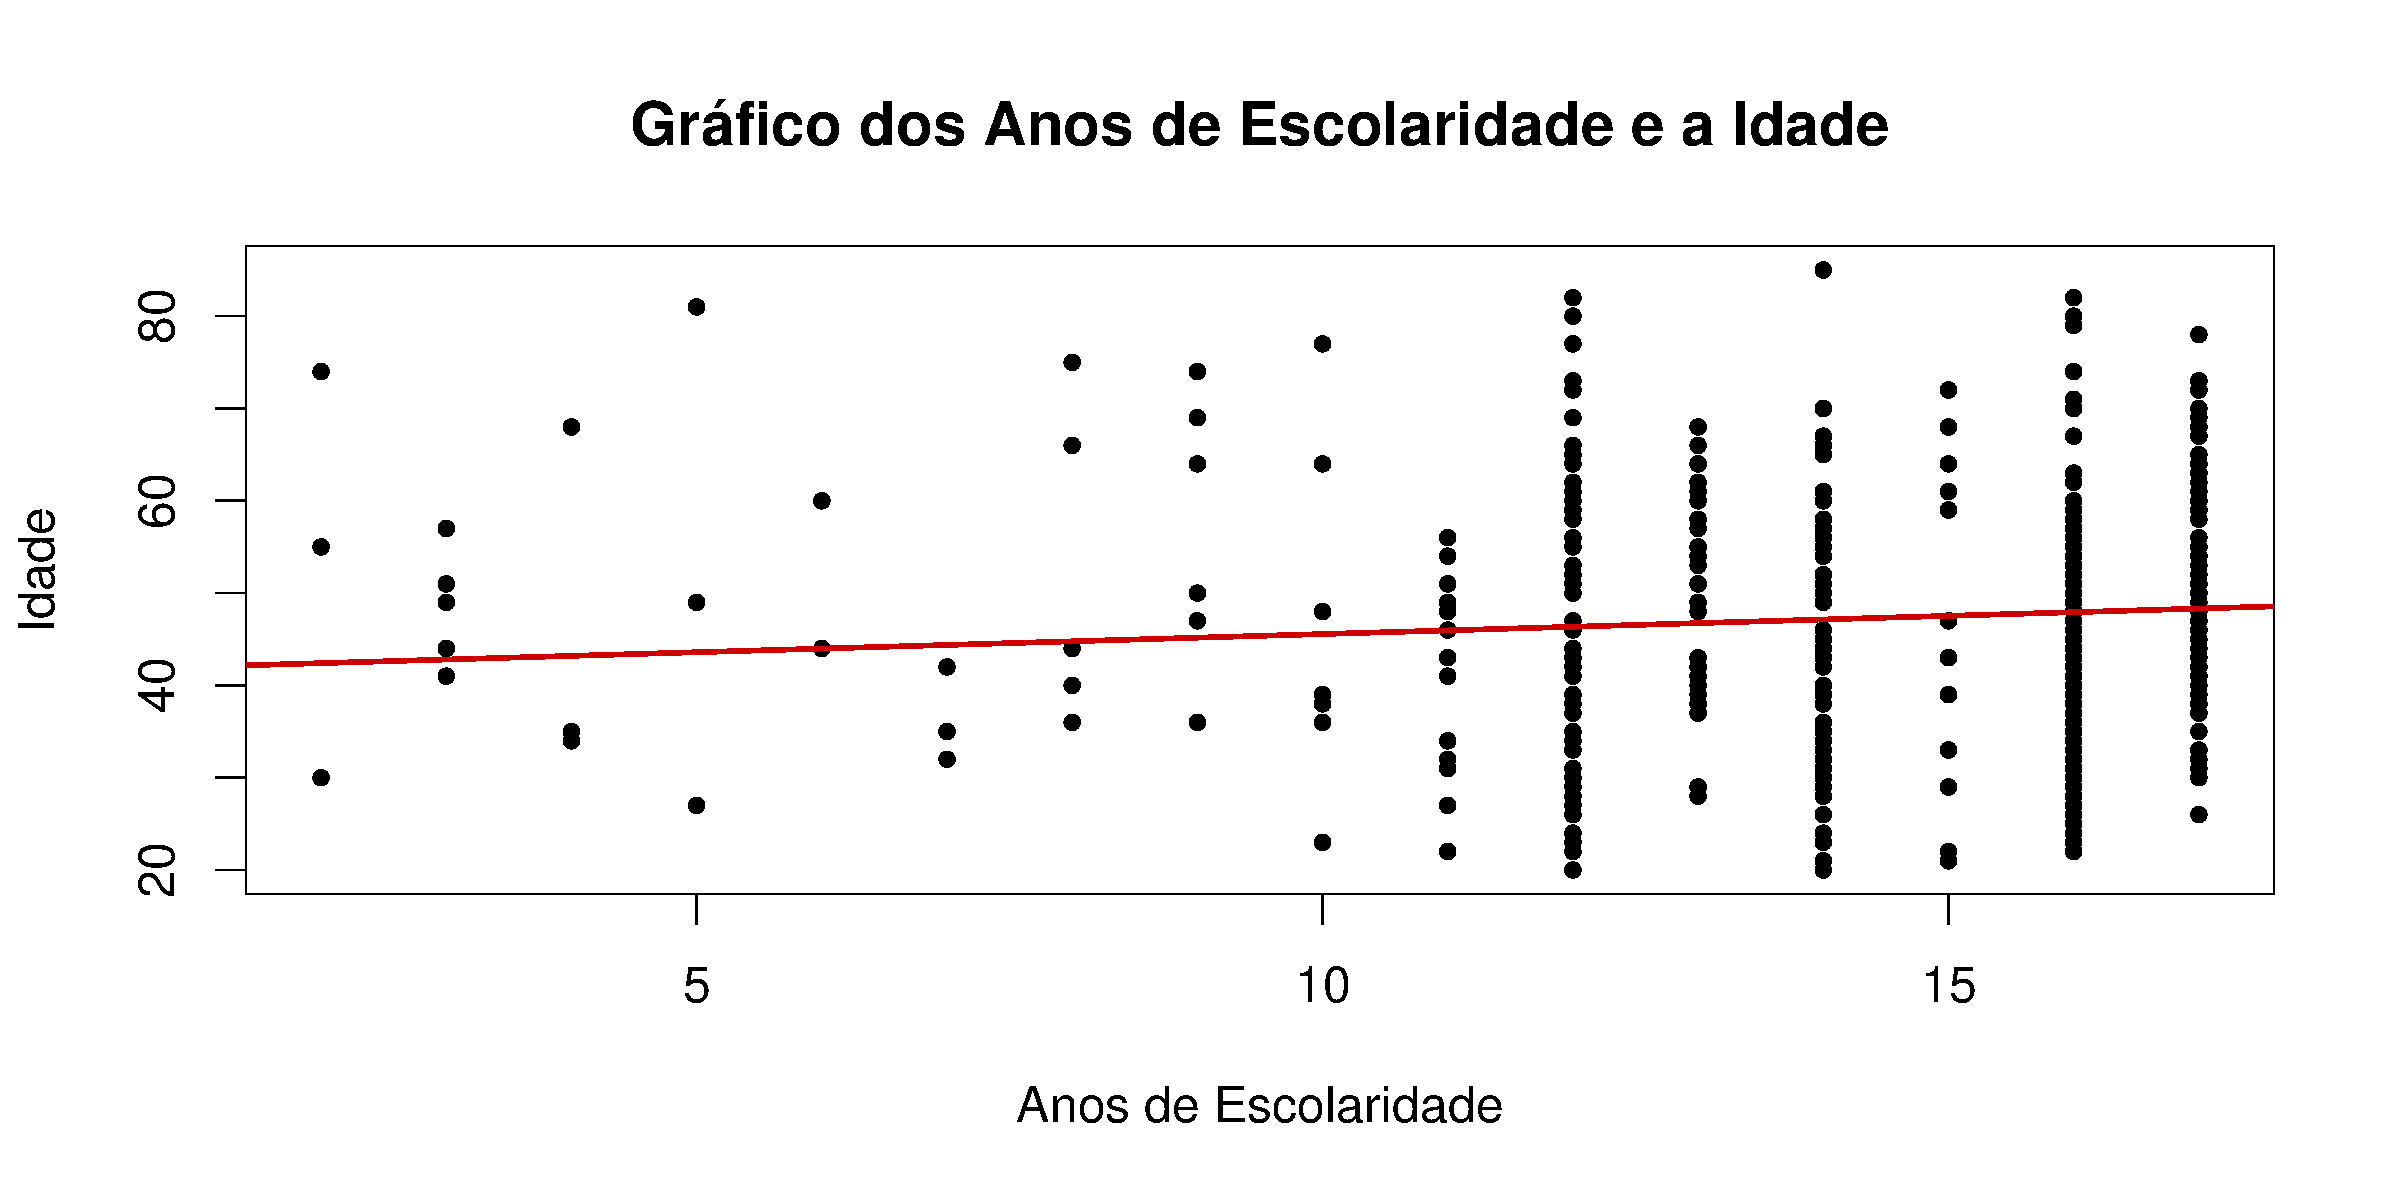
\includegraphics[width=0.6\linewidth]{p27-graf} 

}

\caption{Distribuição da Idade pelos Anos de Escolaridade.}\label{fig:unnamed-chunk-13}
\end{figure}

Analisando as variáveis Anos de Escolaridade e a Idade, percebemos um
aumento na inclinação quando aumenta os anos de escolaridade e as idades
dos entrevistados, ou seja, os entrevistados possuem maior anos de
escolaridade à medida que aumentam as idades, o que condiz com a
realidade dos ensinos visto anteriormente. Embora quantidades de anos de
escolaridade maior possuem grande concentração de pessoas em diversas
idades, para os anos de escolaridade entre 2-10 anos percebemos a
presença de variabilidade, conforme a Figura 6.

\begin{figure}[H]

{\centering 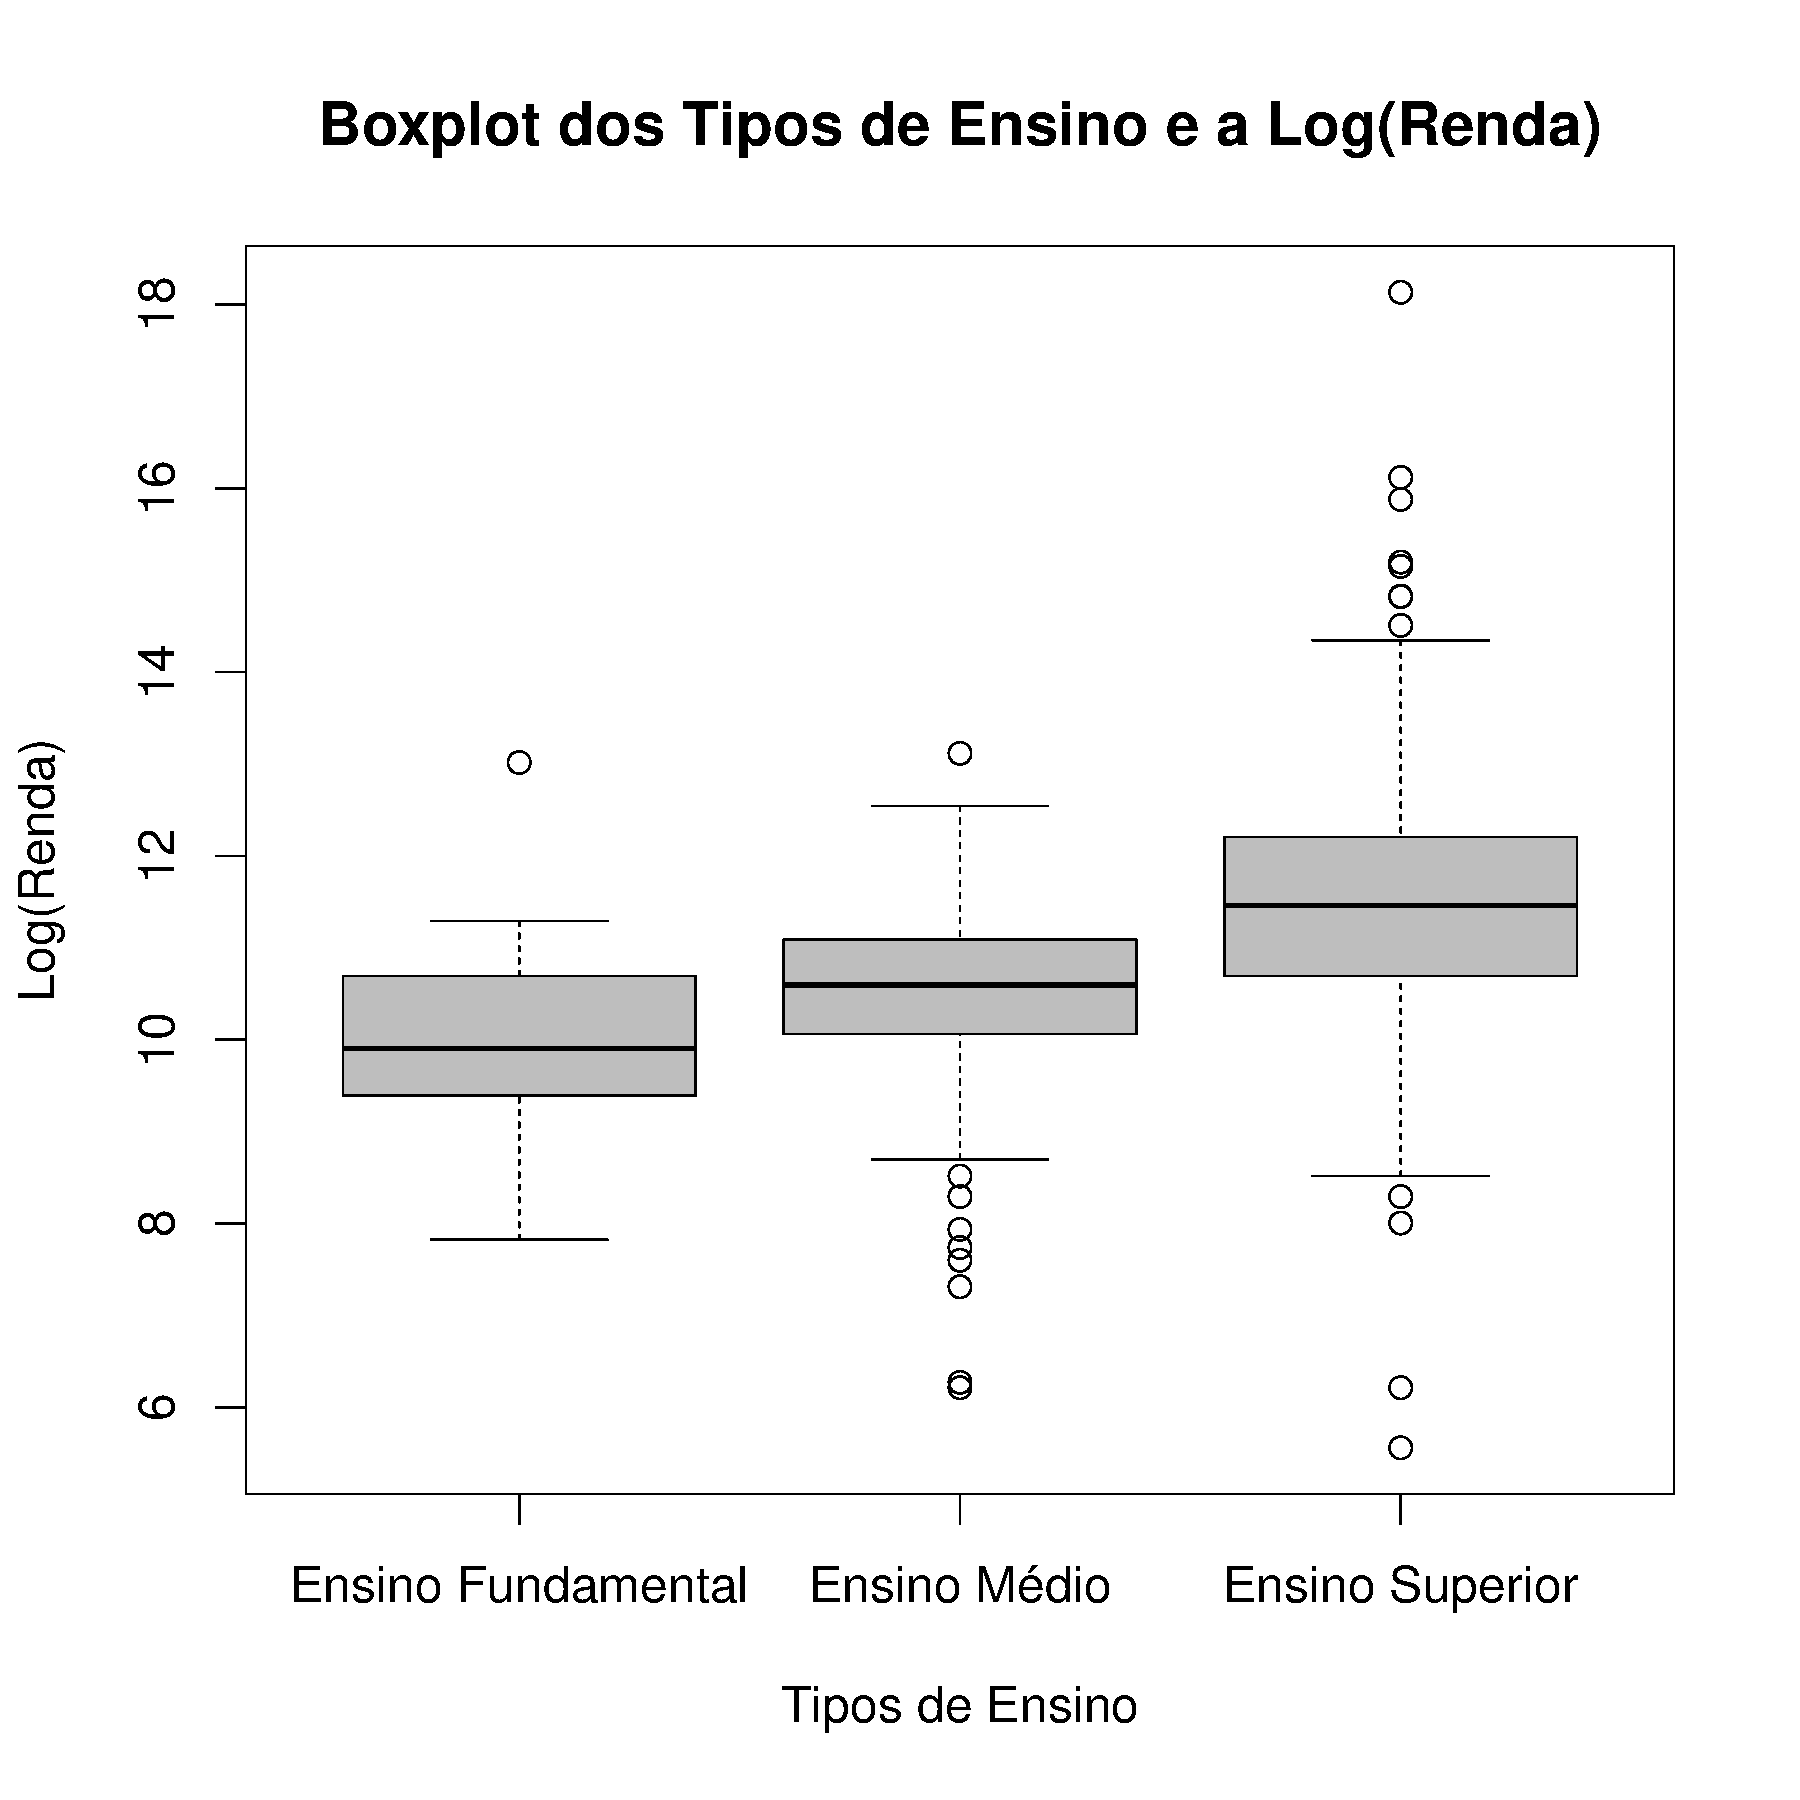
\includegraphics[width=0.6\linewidth]{p21-graf} 

}

\caption{Box-plots da Log(Renda) pelos Tipos de Ensino.}\label{fig:unnamed-chunk-14}
\end{figure}

Avaliando a relação entre as variáveis Log(Renda) e a recodificação da
variável Anos de Escolaridade, variável separada em tipos de ensino para
melhor visualização da relação existente, temos que o tipo de ensino
influencia na renda dos entrevistados. Assim observamos valores de renda
maiores para o Ensino Superior, que possui de 15-17 anos de
escolaridade, conforme Figura 7.

Após a apresentação das variáveis individualmente e em pares com a
variável de interesse renda anual, realizamos a análise das variáveis em
trios, como por exemplo a Log(Renda), Idade e o Gênero. As análises da
relação dessas variáveis permitem fazer suposições sobre os modelos a
serem estudados e verificar a influência de cada covariável na variável
resposta.

\begin{figure}[H]

{\centering 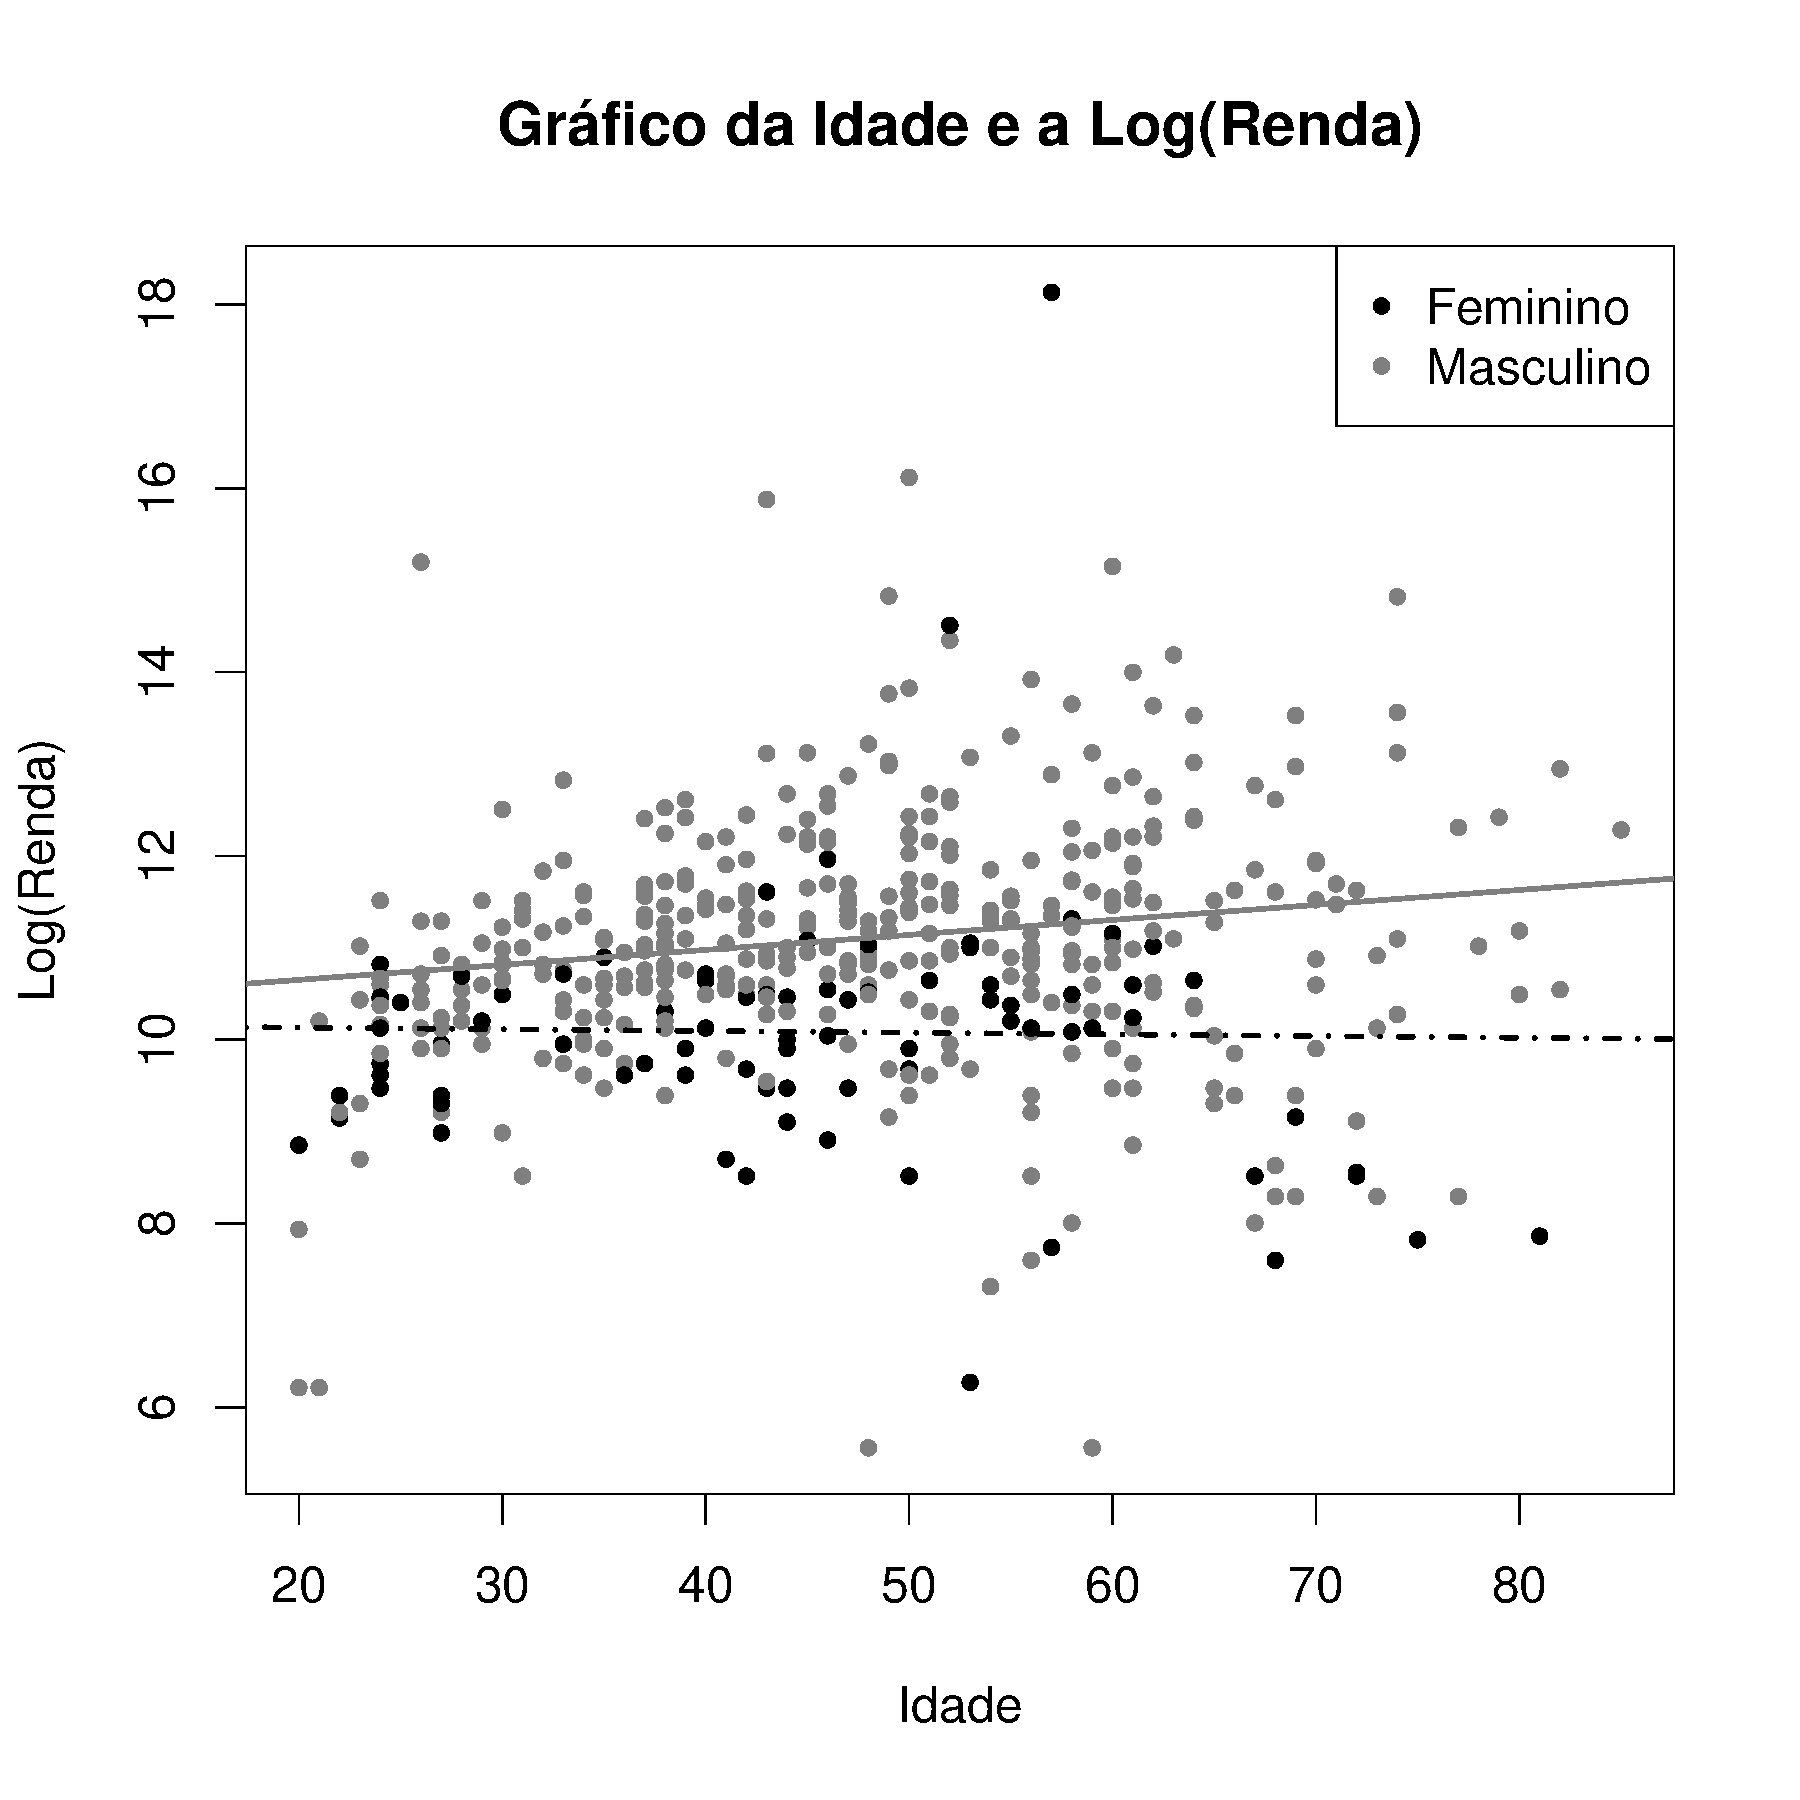
\includegraphics[width=0.6\linewidth]{p17-graf} 

}

\caption{Distribuição da Log(Renda) pela Idade, decomposta pelo Gênero.}\label{fig:unnamed-chunk-15}
\end{figure}

Analisando a relação entre as variáveis Log(Renda), Idade e Gênero
percebemos o quanto a idade e o gênero influenciam nos valores da renda
anual. A Figura 8 possui o ajuste das retas e mostra claramente o que
foi discutido anteriormente, sobre os valores de renda anual para o sexo
masculino serem maiores que o do sexo feminino; podemos perceber também
uma inclinação na reta à medida que aumenta a idade para o sexo
masculino, entretanto para as mulheres essa inclinação é muito pequena
ou inexistente.

\begin{figure}[H]

{\centering 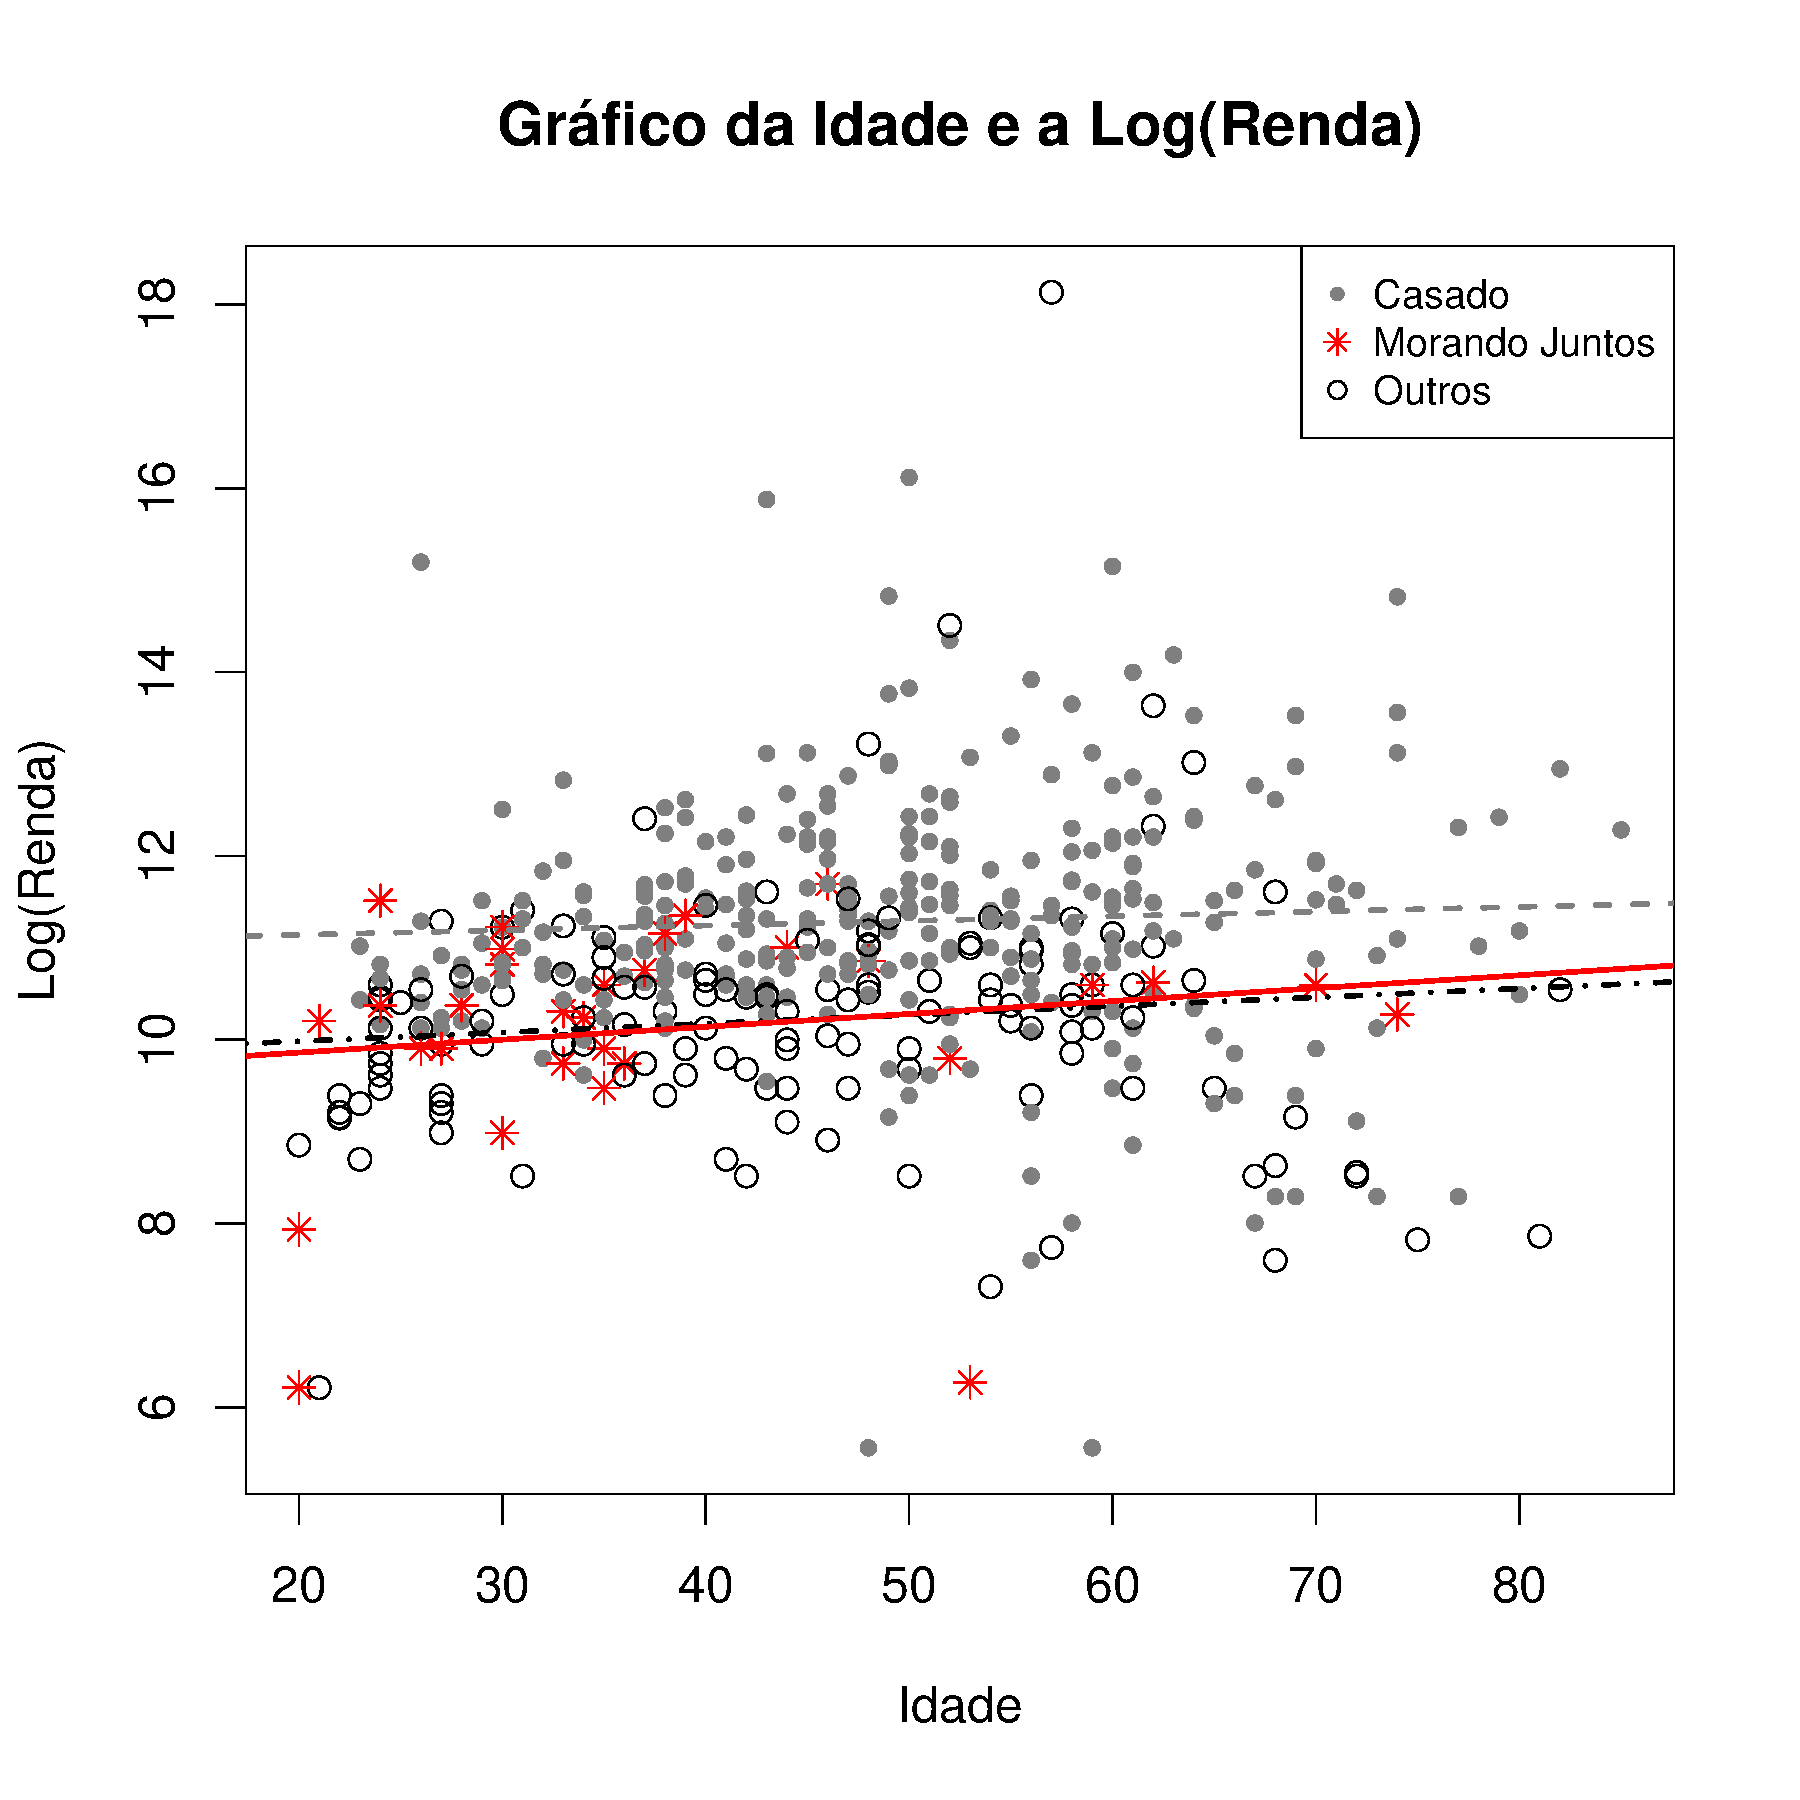
\includegraphics[width=0.6\linewidth]{p18-graf} 

}

\caption{Distribuição da Log(Renda) pela Idade, decomposta pelo Estado Civil.}\label{fig:unnamed-chunk-16}
\end{figure}

Para a análise entre as variáveis Log(Renda), Idade e Estado Civil,
podemos observar que os entrevistados casados possuem uma quantidade
maior de renda e através da inclinação da reta podemos concluir que a
renda aumenta através da idade, já para os entrevistados que estão
morando juntos e os outros tipos de estado civil as retas e a inclinação
estão quase juntas, sendo que possuem pequenas diferenças em algumas
idades; a Figura 9 também mostra como está a distribuição por estado
civil dos entrevistados.

\begin{figure}[H]

{\centering 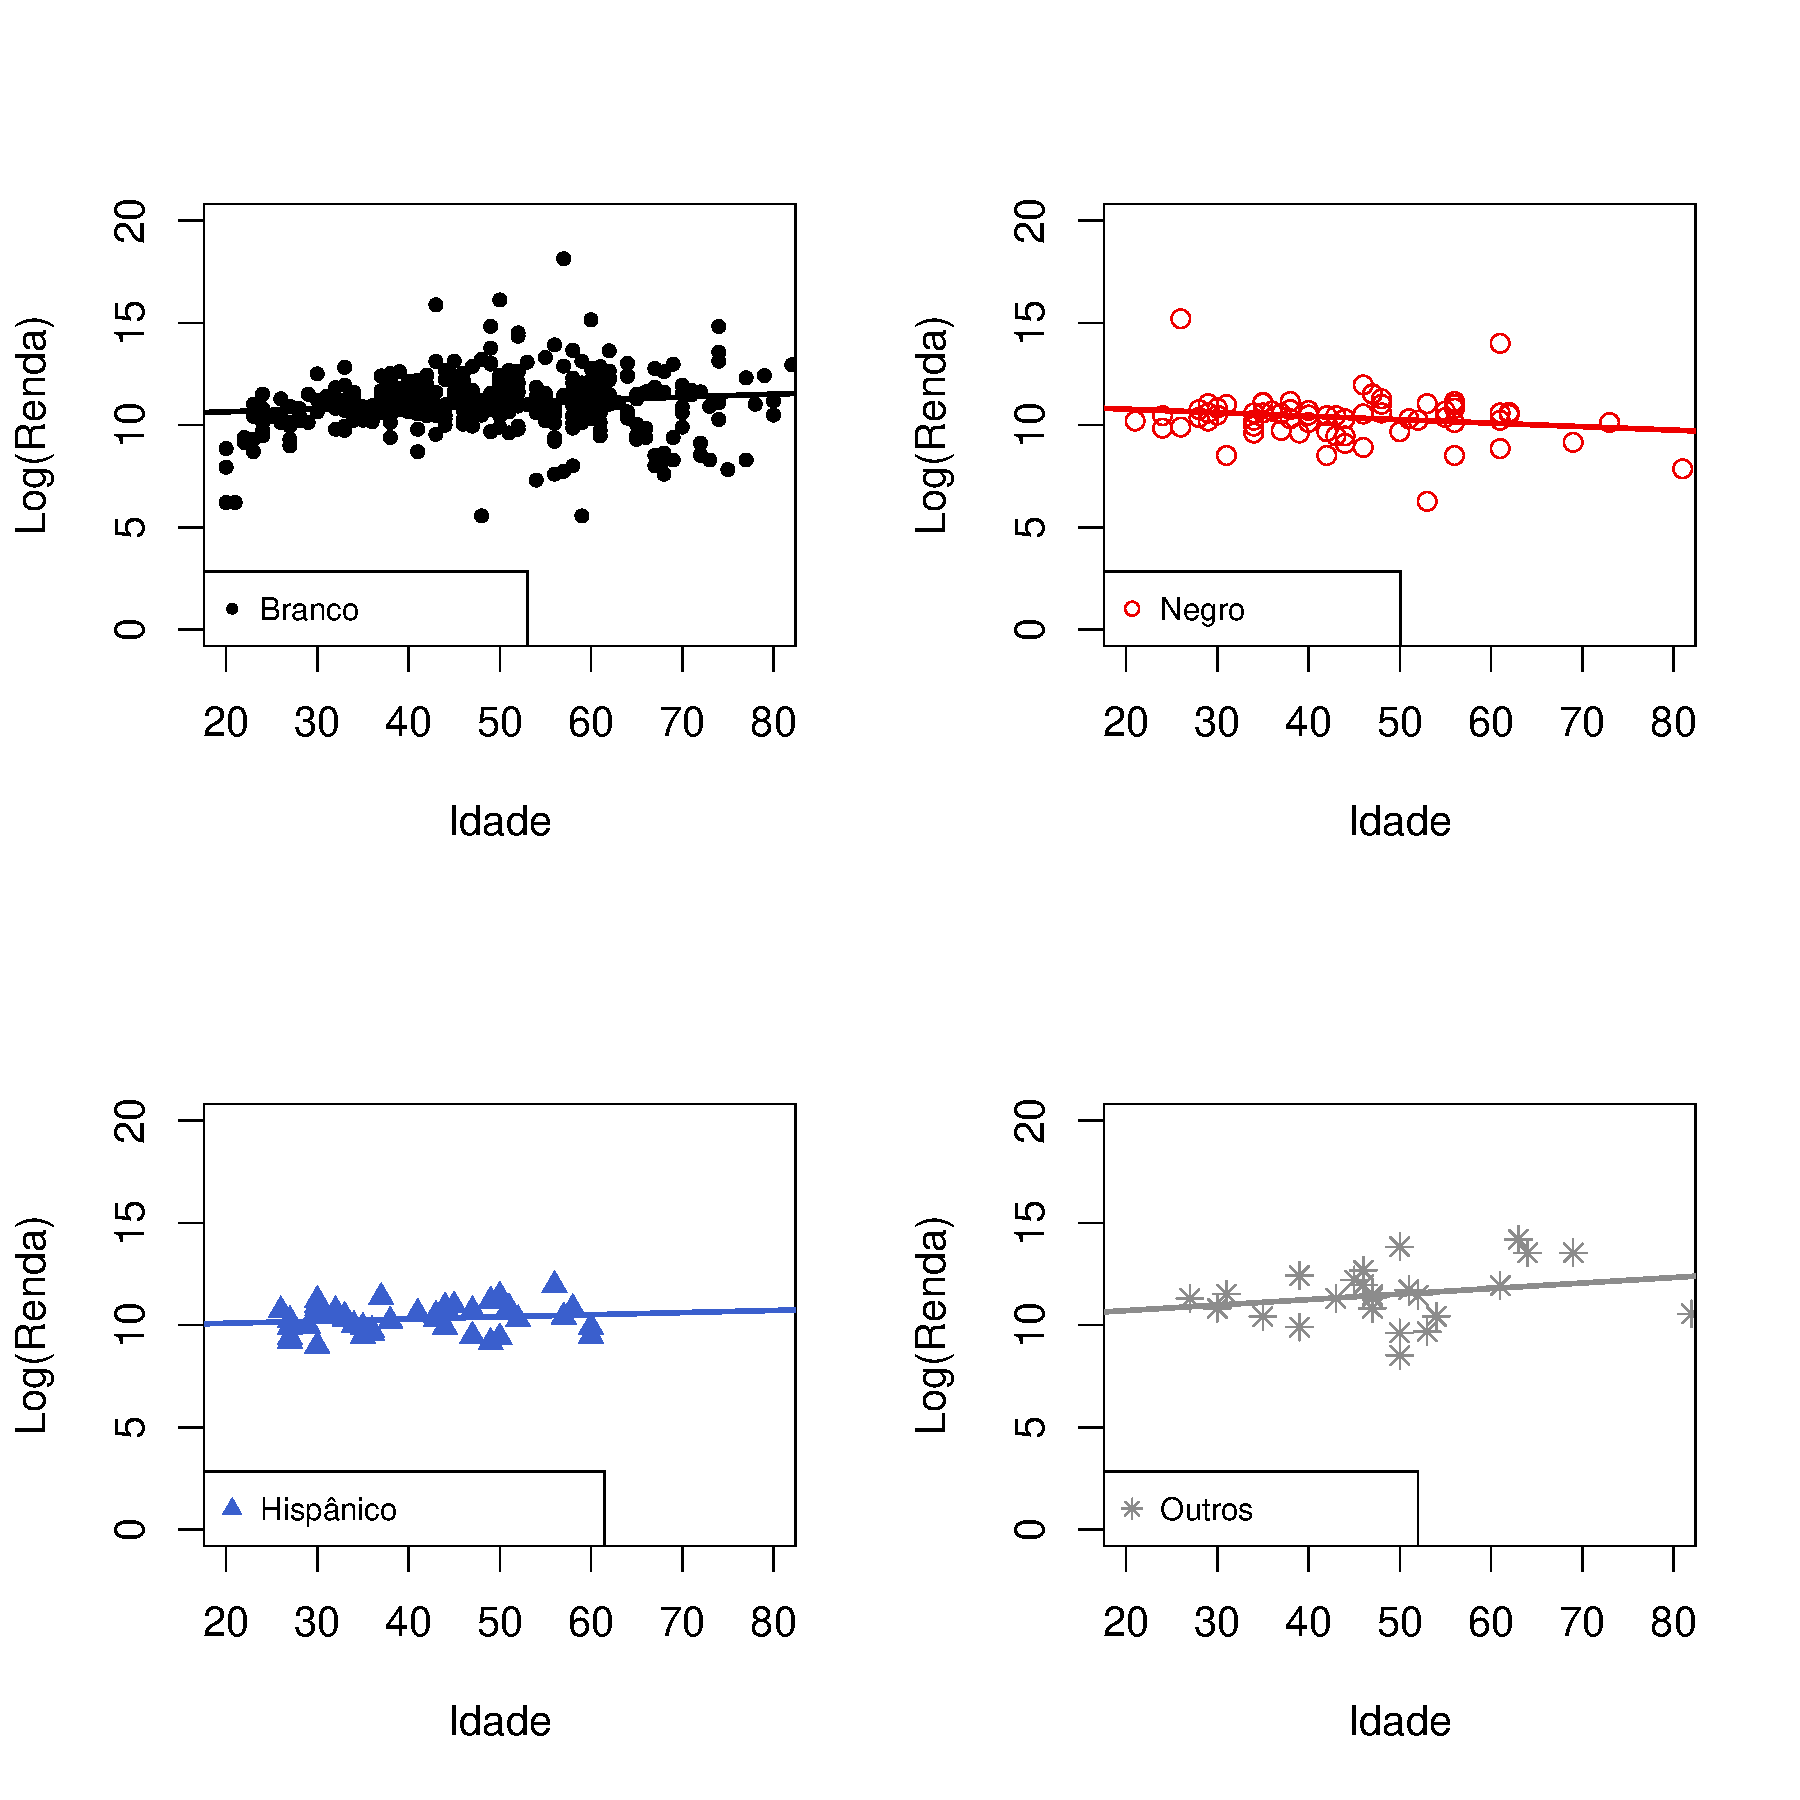
\includegraphics[width=0.6\linewidth]{p28-graf} 

}

\caption{Distribuição da Log(Renda) pela Idade, decomposta pela Etnia.}\label{fig:unnamed-chunk-17}
\end{figure}

Analisando a relação entre as variáveis Log(Renda), Idade e a Etnia,
vemos que as retas pertencentes as etnias Branco, Negro e Outros partem
quase do mesmo valor de renda, entretanto, ao longo das idades, possuem
comportamentos diferentes para a inclinação da reta, sendo que para a
etnia Negro a renda decresce a medida que aumenta a idade. Observamos
maior renda para a etnia Outros; já a etnia Hispânico, que começa a reta
abaixo das outras etnias, intercepta a etnia Negro entre as idades 40-50
anos. Pelo gráfico da distribuição da Figura 10 percebemos que as
observações da etnia Hispânico estão concentrados em torno do Log(Renda)
igual a 10, e que a etnia Negro possue valores de renda bastante
dispersos a medida que aumenta a idade.

\begin{figure}[H]

{\centering 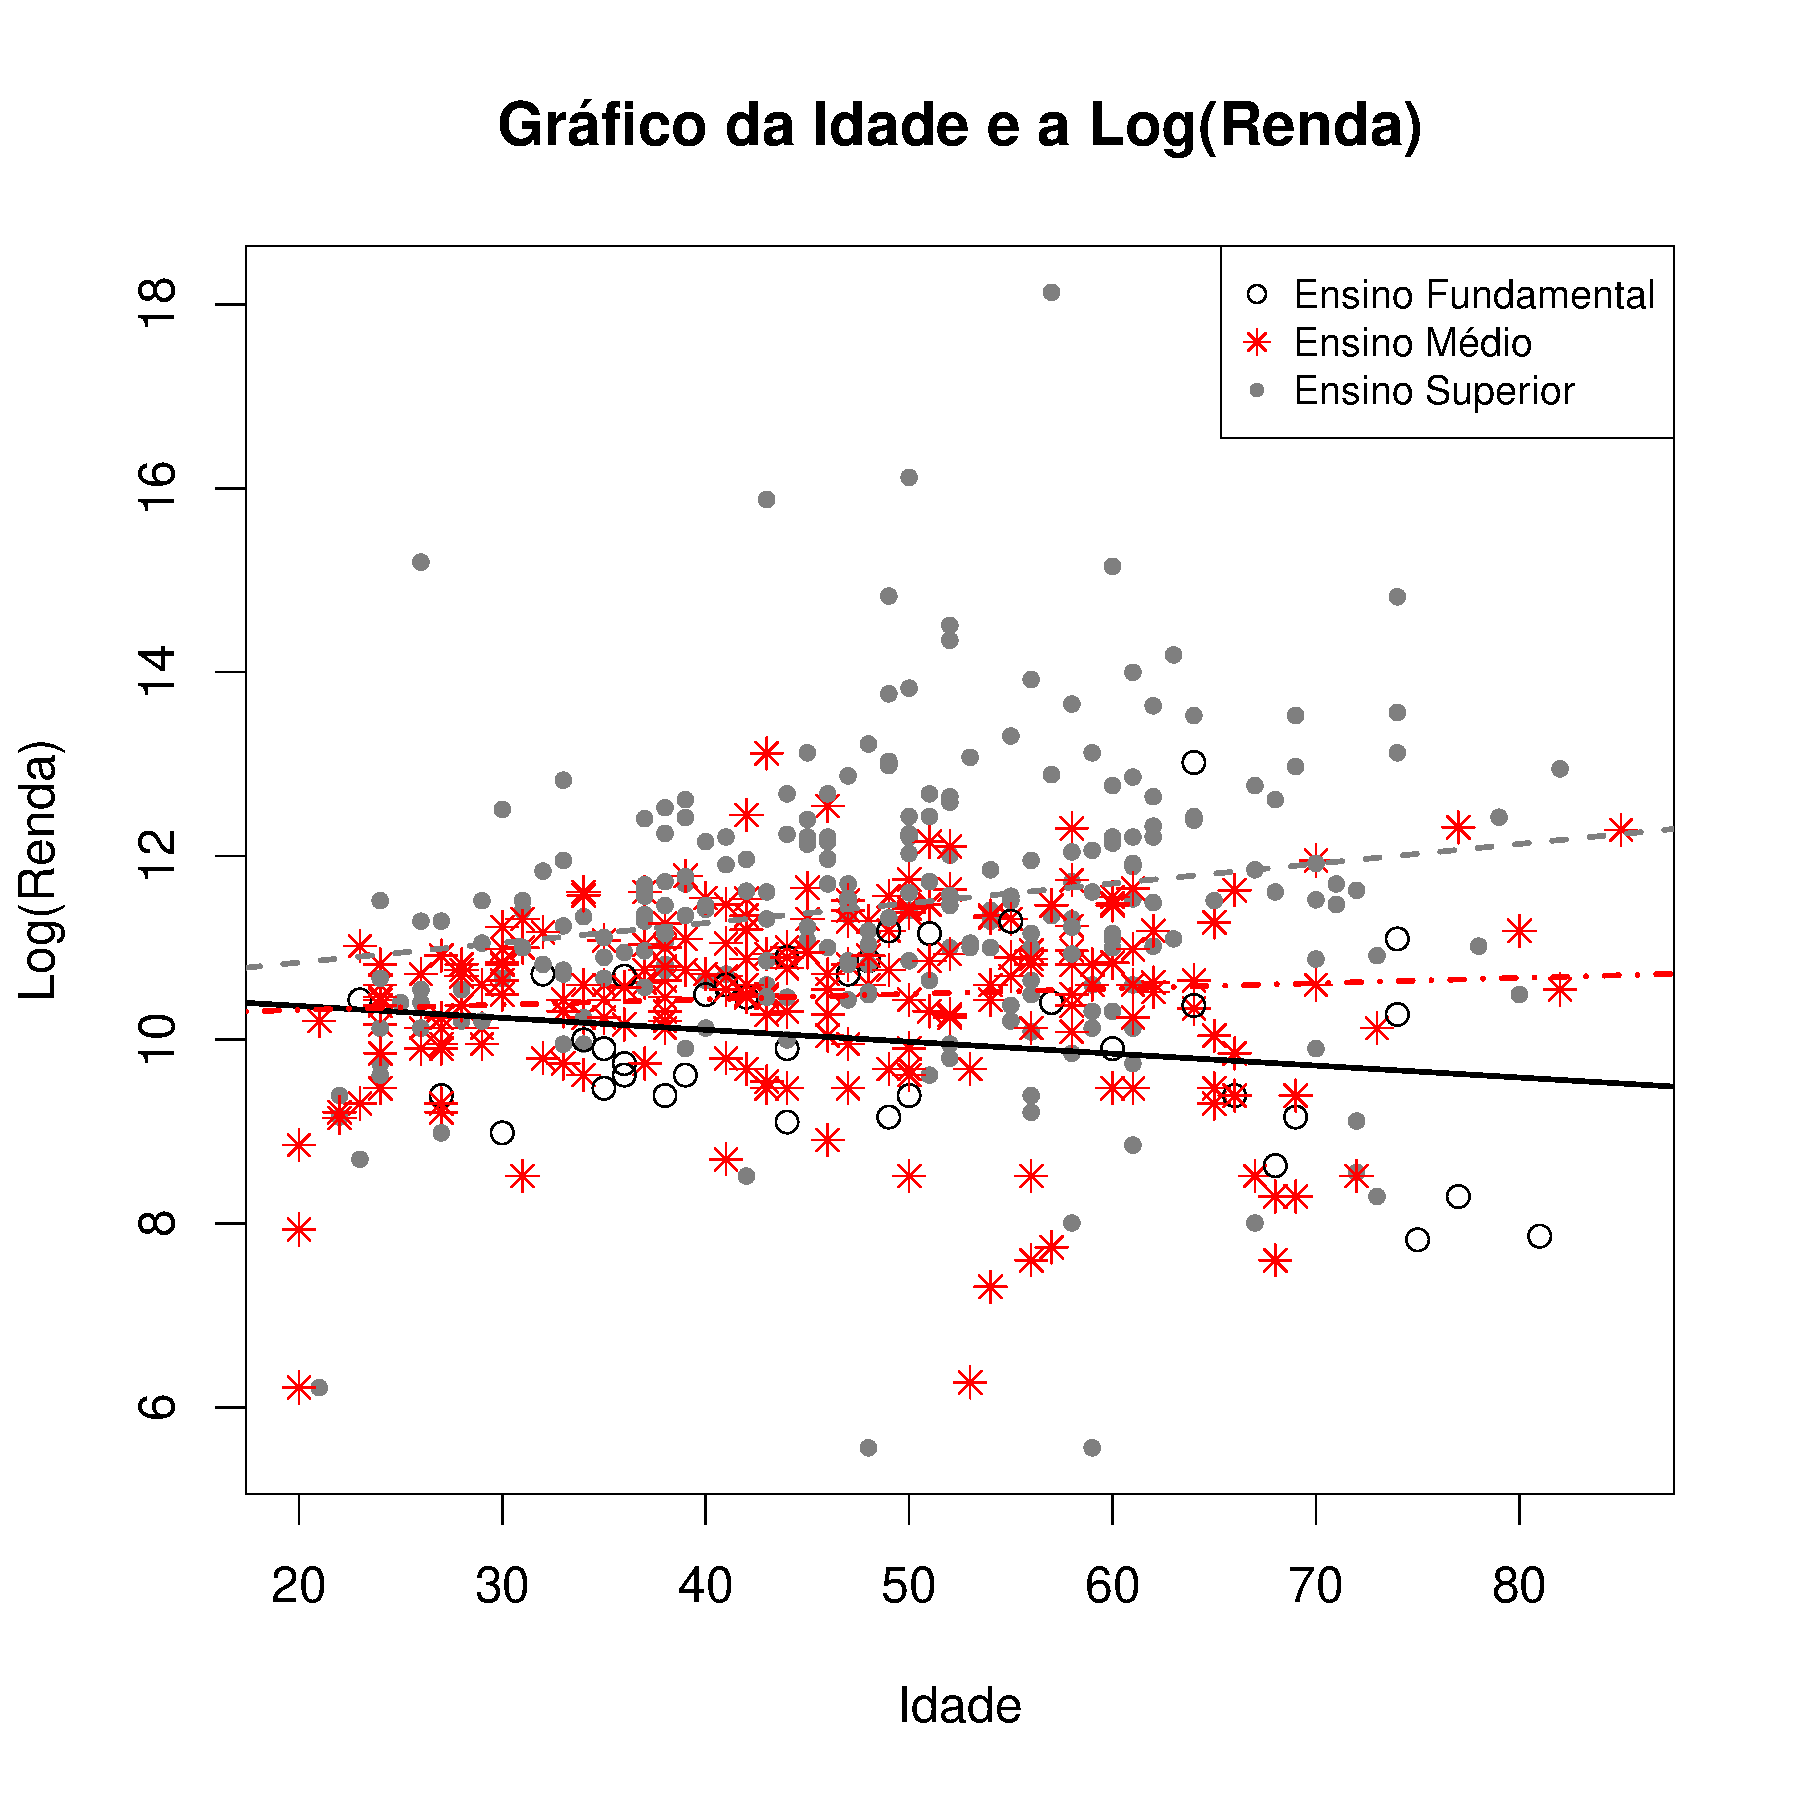
\includegraphics[width=0.6\linewidth]{p22-graf} 

}

\caption{Distribuição da Log(Renda) pela Idade, decomposta pelo Tipo de Ensino.}\label{fig:unnamed-chunk-18}
\end{figure}

Para a análise entre as variáveis Log(Renda), Idade e os Tipos de
Ensino, confirmamos a conclusão anterior sobre o Ensino Superior possuir
renda maior que os outros tipos de ensino. Nas idades mais jovens, a
renda para o Ensino Fundamental e o Ensino Médio estão muito próximas
quando analisamos a inclinação da reta, entretanto a partir dos 30 anos
as retas desses dois tipos de ensino começam a se distanciar; há um
aumento de renda para o Ensino Médio enquanto o Ensino Fundamental
apresenta declínio, conforme a Figura 11.

\subsection{Imputação}\label{imputacao}

\subsubsection{Perda Completamente Aleatória
(PCA)}\label{perda-completamente-aleatoria-pca}

No mecanismo de PCA, utilizamos uma Distribuição Bernoulli com
probabilidade de sucesso (p) de 0,20 para gerar os dados ausentes na
variável Renda, e fixamos uma semente ao gerar os números aleatórios. Ao
final obtivemos um banco de dados com 96 observações ausentes das 500
observações existentes no banco de dados, os dados ausentes foram
gerados de acordo com a metodologia descrita na seção 2.

Pelos box-plots da Figura 12 podemos verificar os valores da Renda do
banco de dados original, do banco de dados gerado com valores ausentes
(através do mecanismo PCA) e as cinco imputações geradas.

\begin{figure}[H]

{\centering 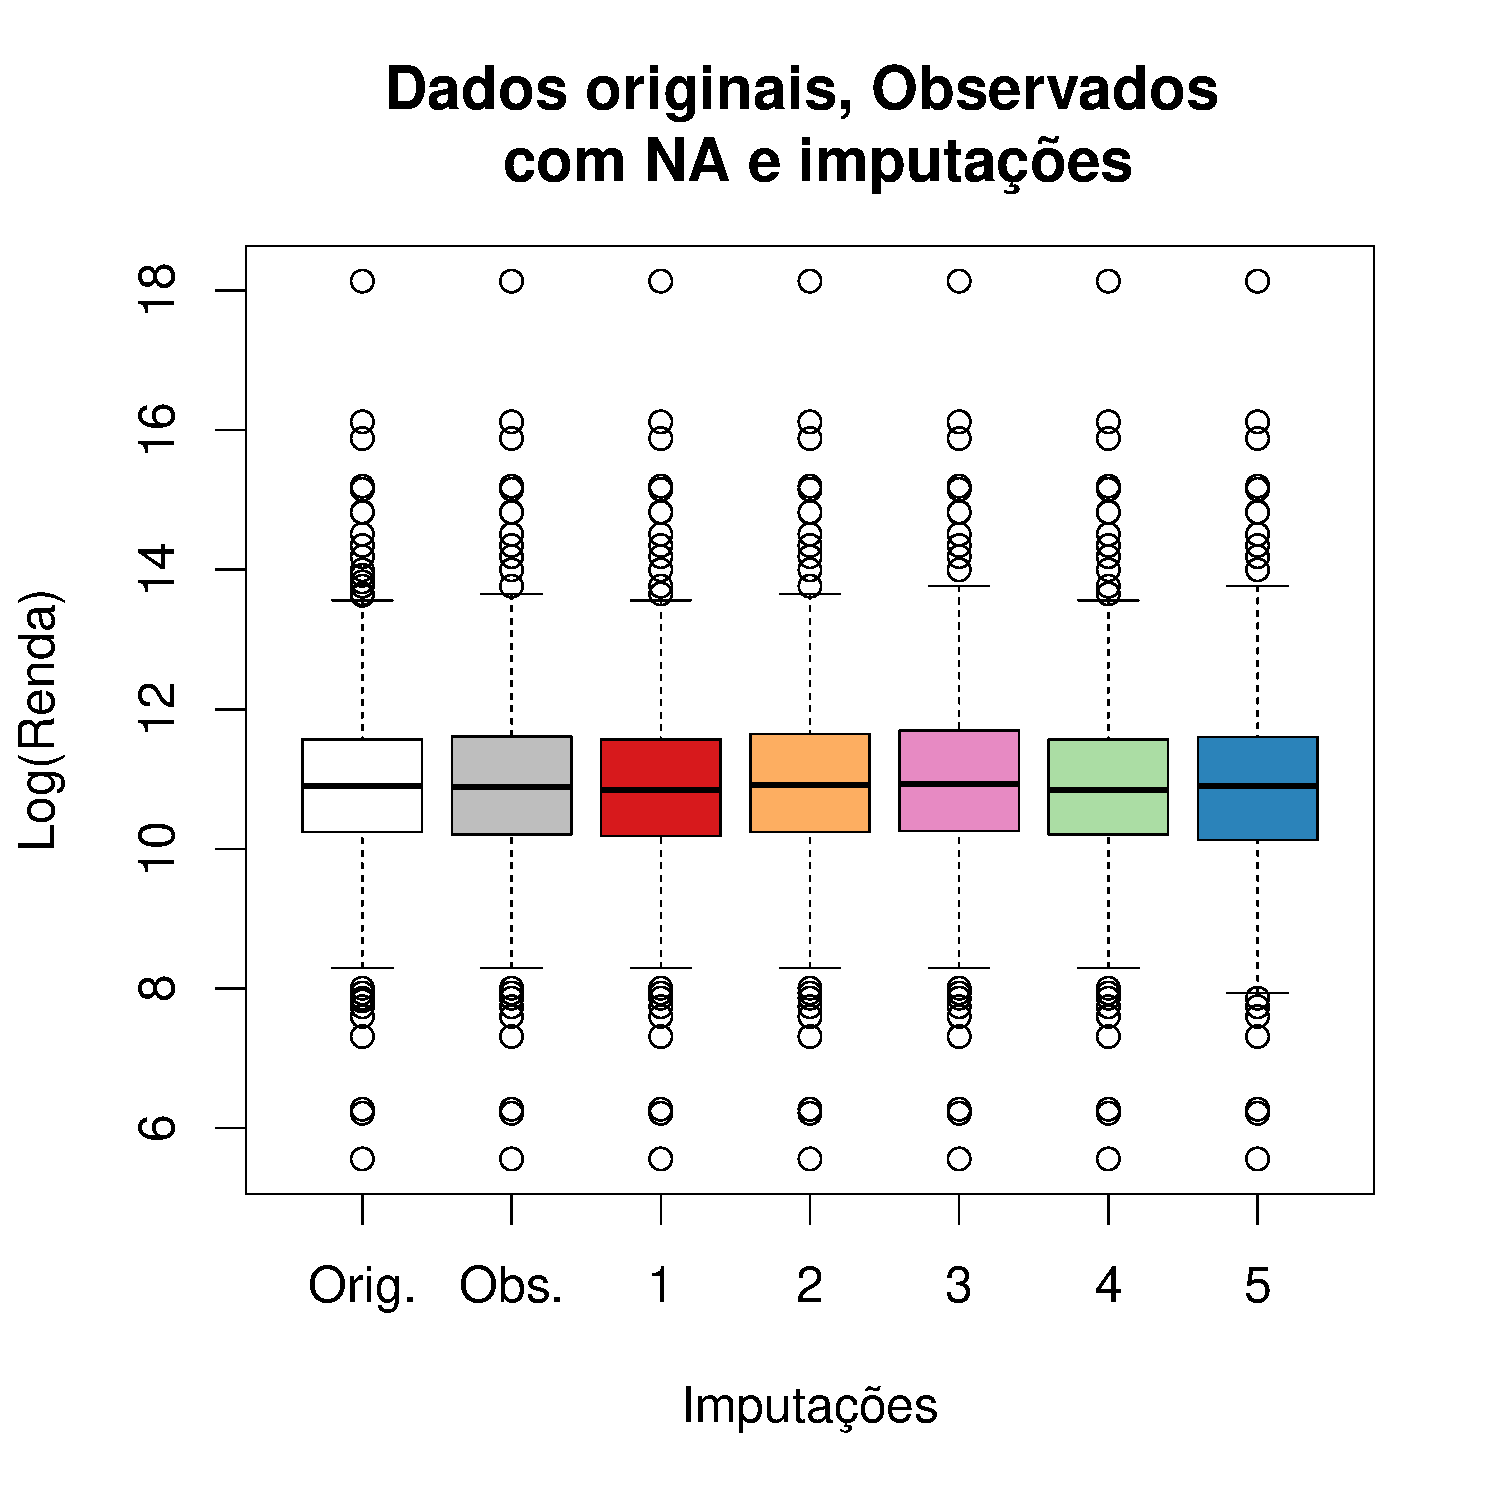
\includegraphics[width=0.6\linewidth]{p57-graf} 

}

\caption{Box-plots dos dados originais, dados observados com valores ausentes e as 5 imputações geradas.}\label{fig:unnamed-chunk-20}
\end{figure}

Nos box-plots da Figura 12 percebemos que as cinco imputações geradas
seguem de modo semelhante a distribuição do banco com os valores
ausentes. Temos também que os valores originais e os valores imputados
estão bastante próximos. Podemos verificar também através da
distribuição do banco de dados original com os bancos de dados das
imputações através da Figura 13. Pelo gráfico de dispersão da Figura 13,
confirmamos que os valores orignais e os valores imputados estão
bastante próximos.

\begin{figure}[H]

{\centering 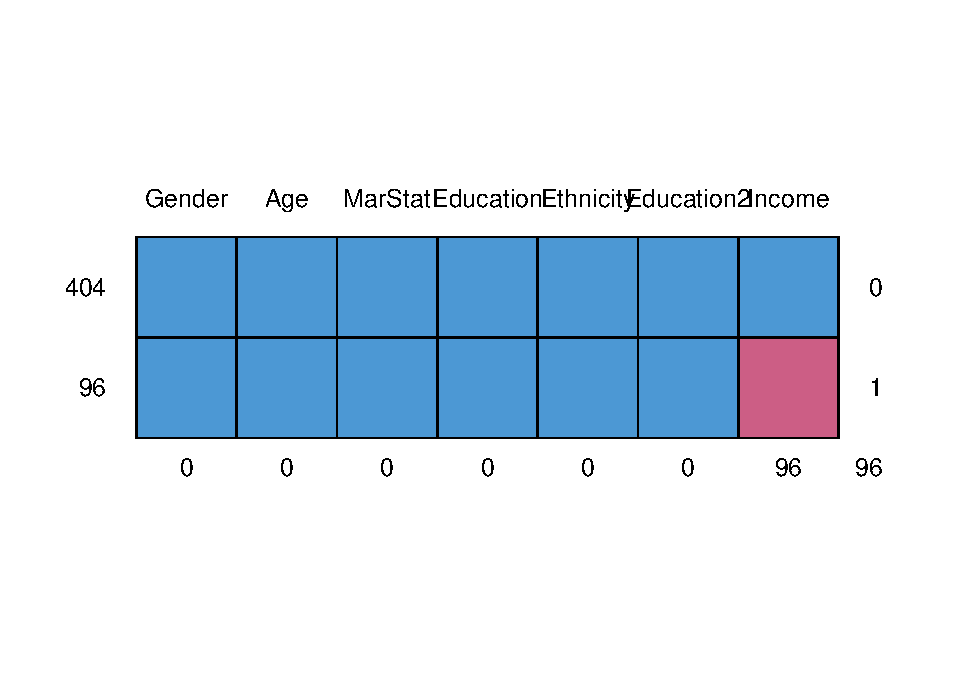
\includegraphics[width=0.6\linewidth]{Relatorio_IC_files/figure-latex/unnamed-chunk-21-1} 

}

\caption{Distribuição da Log(Renda) pelos dados originais e as imputações, as observações foram decompostas em observações originais e ausentes imputadas.}\label{fig:unnamed-chunk-21}
\end{figure}

\begin{figure}[H]

{\centering 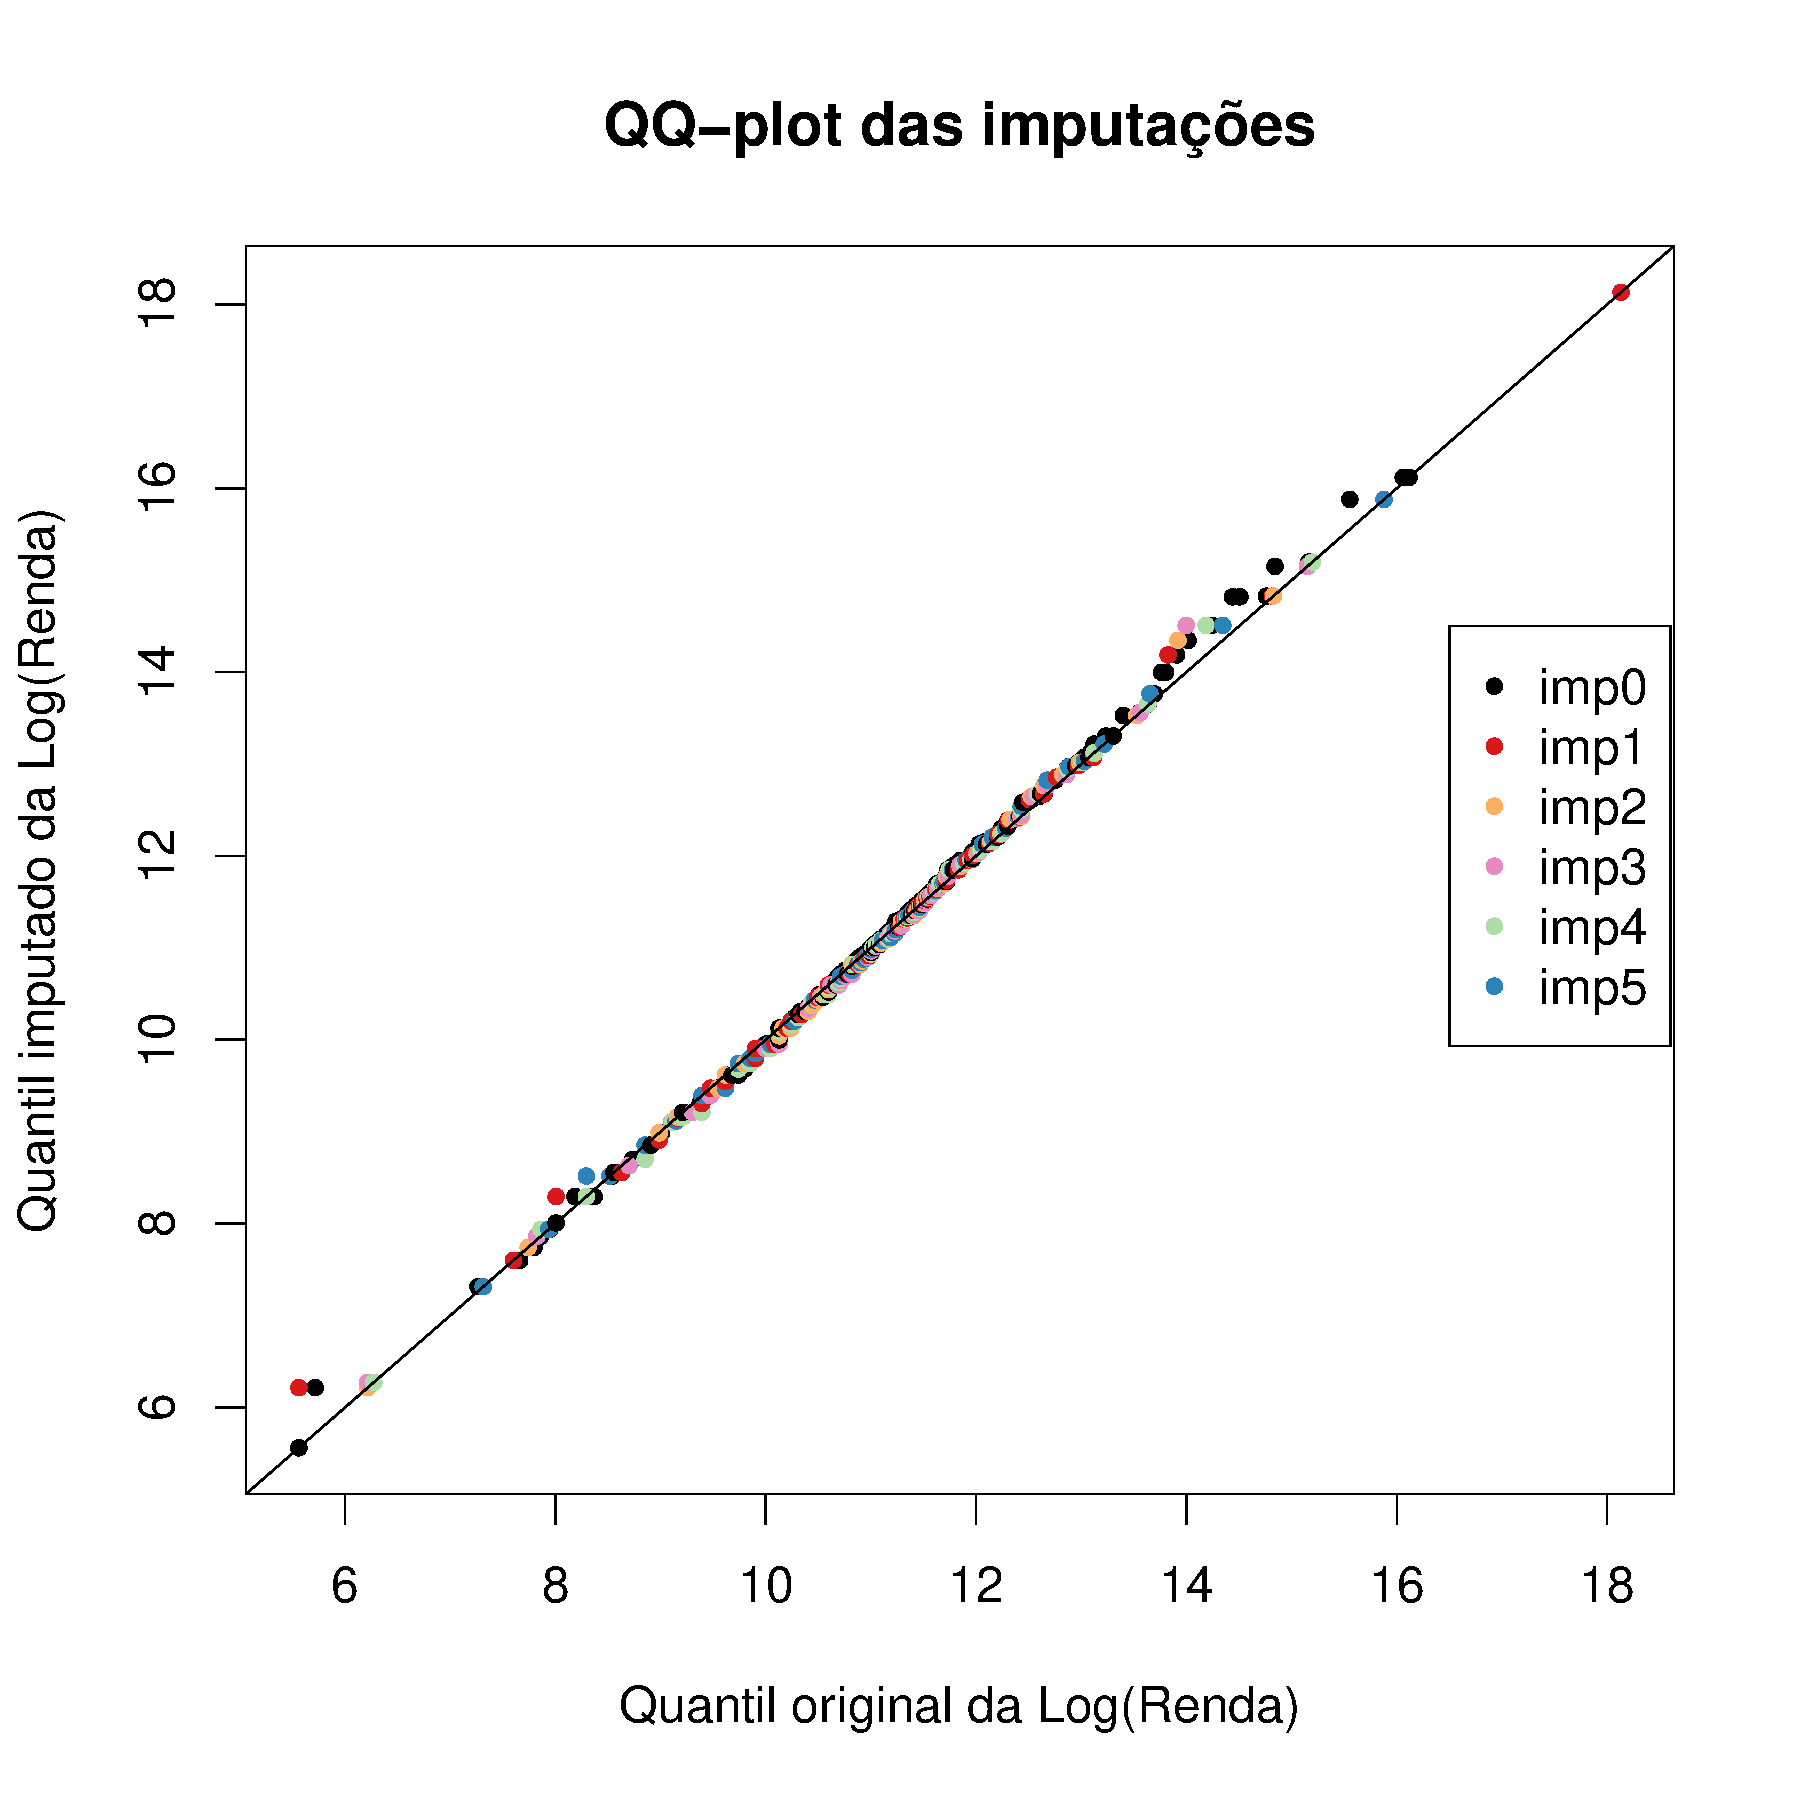
\includegraphics[width=0.6\linewidth]{p43-graf} 

}

\caption{QQ-plot das imputações, quantil imputado da Log(Renda) pelo quantil observado da Log(Renda).}\label{fig:unnamed-chunk-22}
\end{figure}

Pela Figura 14 podemos checar a adequação do modelo dos dados com as
observações faltantes com as imputações realizadas. Nele vemos que os
valores estão bastante concentrados indicando que os valores imputados
são adequados.

\subsubsection{Perda Aleatória (PA)}\label{perda-aleatoria-pa}

Para gerar os dados ausentes do mecanismo de PA, avaliamos a perda da
variável Renda conjuntamente com as variáveis Gênero e Tipo de Ensino.

\paragraph{Gênero}\label{genero}

Para gerar os dados ausentes na renda, pelo caso de PA conjuntamente com
o gênero, utilizamos uma Distribuição Bernoulli com probabilidade de
sucesso (p) de 0,10 para o sexo feminino e 0,30 para o sexo masculino, e
fixamos uma semente ao gerar os números aleatórios. Ao final obtivemos
um banco de dados com 127 observações ausentes das 500 observações
existentes no banco de dados.

Os box-plots da Figura 15 indicam como estão a distribuição dos valores
da renda para o banco de dados original, o banco de dados com valores
ausentes na renda e as cinco imputações:

\begin{figure}[H]

{\centering 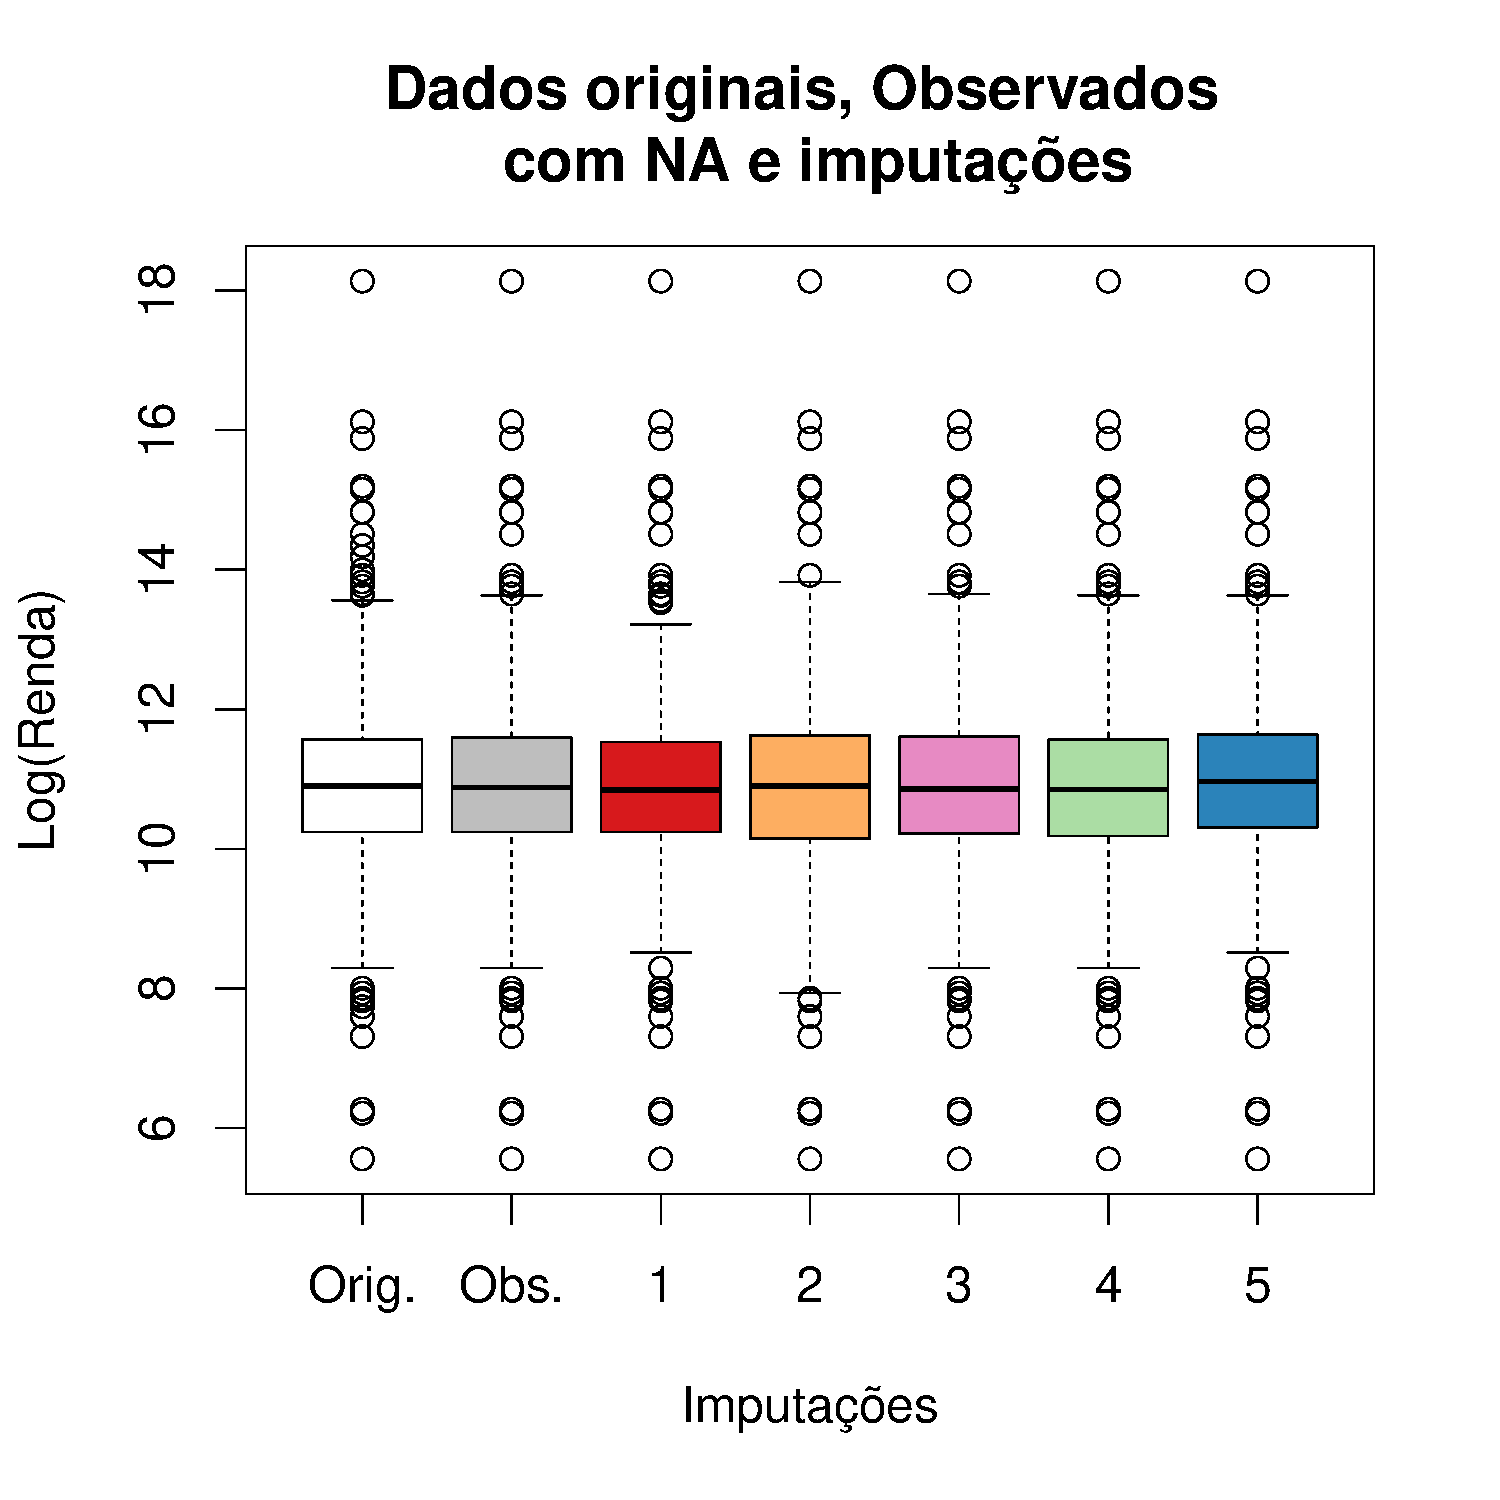
\includegraphics[width=0.6\linewidth]{p56-graf} 

}

\caption{Box-plots dos dados originais, dados observados com valores ausentes e as 5 imputações geradas.}\label{fig:unnamed-chunk-23}
\end{figure}

Pelos box-plots podemos verificar que há pequenos desvios entre eles,
porém as imputações possuem bastante proximidade com o banco de dados
original.

Realizamos a análise dos valores da renda no banco original com os
valores da renda das imputações, e assim obtemos a seguinte
distribuição:

\begin{figure}[H]

{\centering 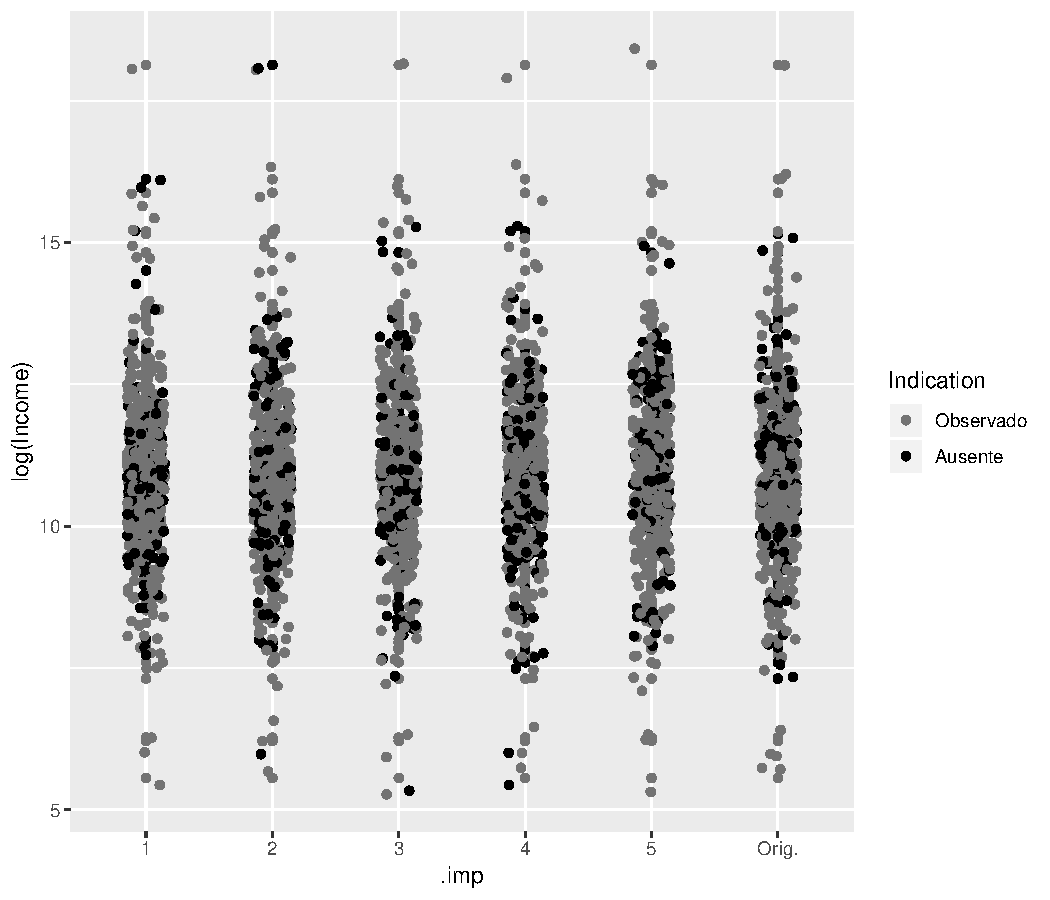
\includegraphics[width=0.6\linewidth]{Relatorio_IC_files/figure-latex/unnamed-chunk-24-1} 

}

\caption{Distribuição da Log(Renda) pelos dados originais e as imputações, as observações foram decompostas em observações originais e ausentes imputadas.}\label{fig:unnamed-chunk-24}
\end{figure}

Pelo gráfico de dispersão da Figura 16 percebemos melhor a distribuição
verificada na Figura 15, novamente observamos indícios de pequenos
desvios entre o banco de dados original e o banco de dados imputado. Nas
imputações 2, 3 e 4 percebemos imputações de valores da log(renda)
próximos de 5, sendo que no banco de dados original não encontramos tais
valores ausentes ao redor do log(renda) igual a 5.

Assim percebemos ainda o indício de pequenos desvios nas imputações
comparada com o banco original. Portanto temos Figura 17 no intuito de
checar a adequação do ajuste:

\begin{figure}[H]

{\centering 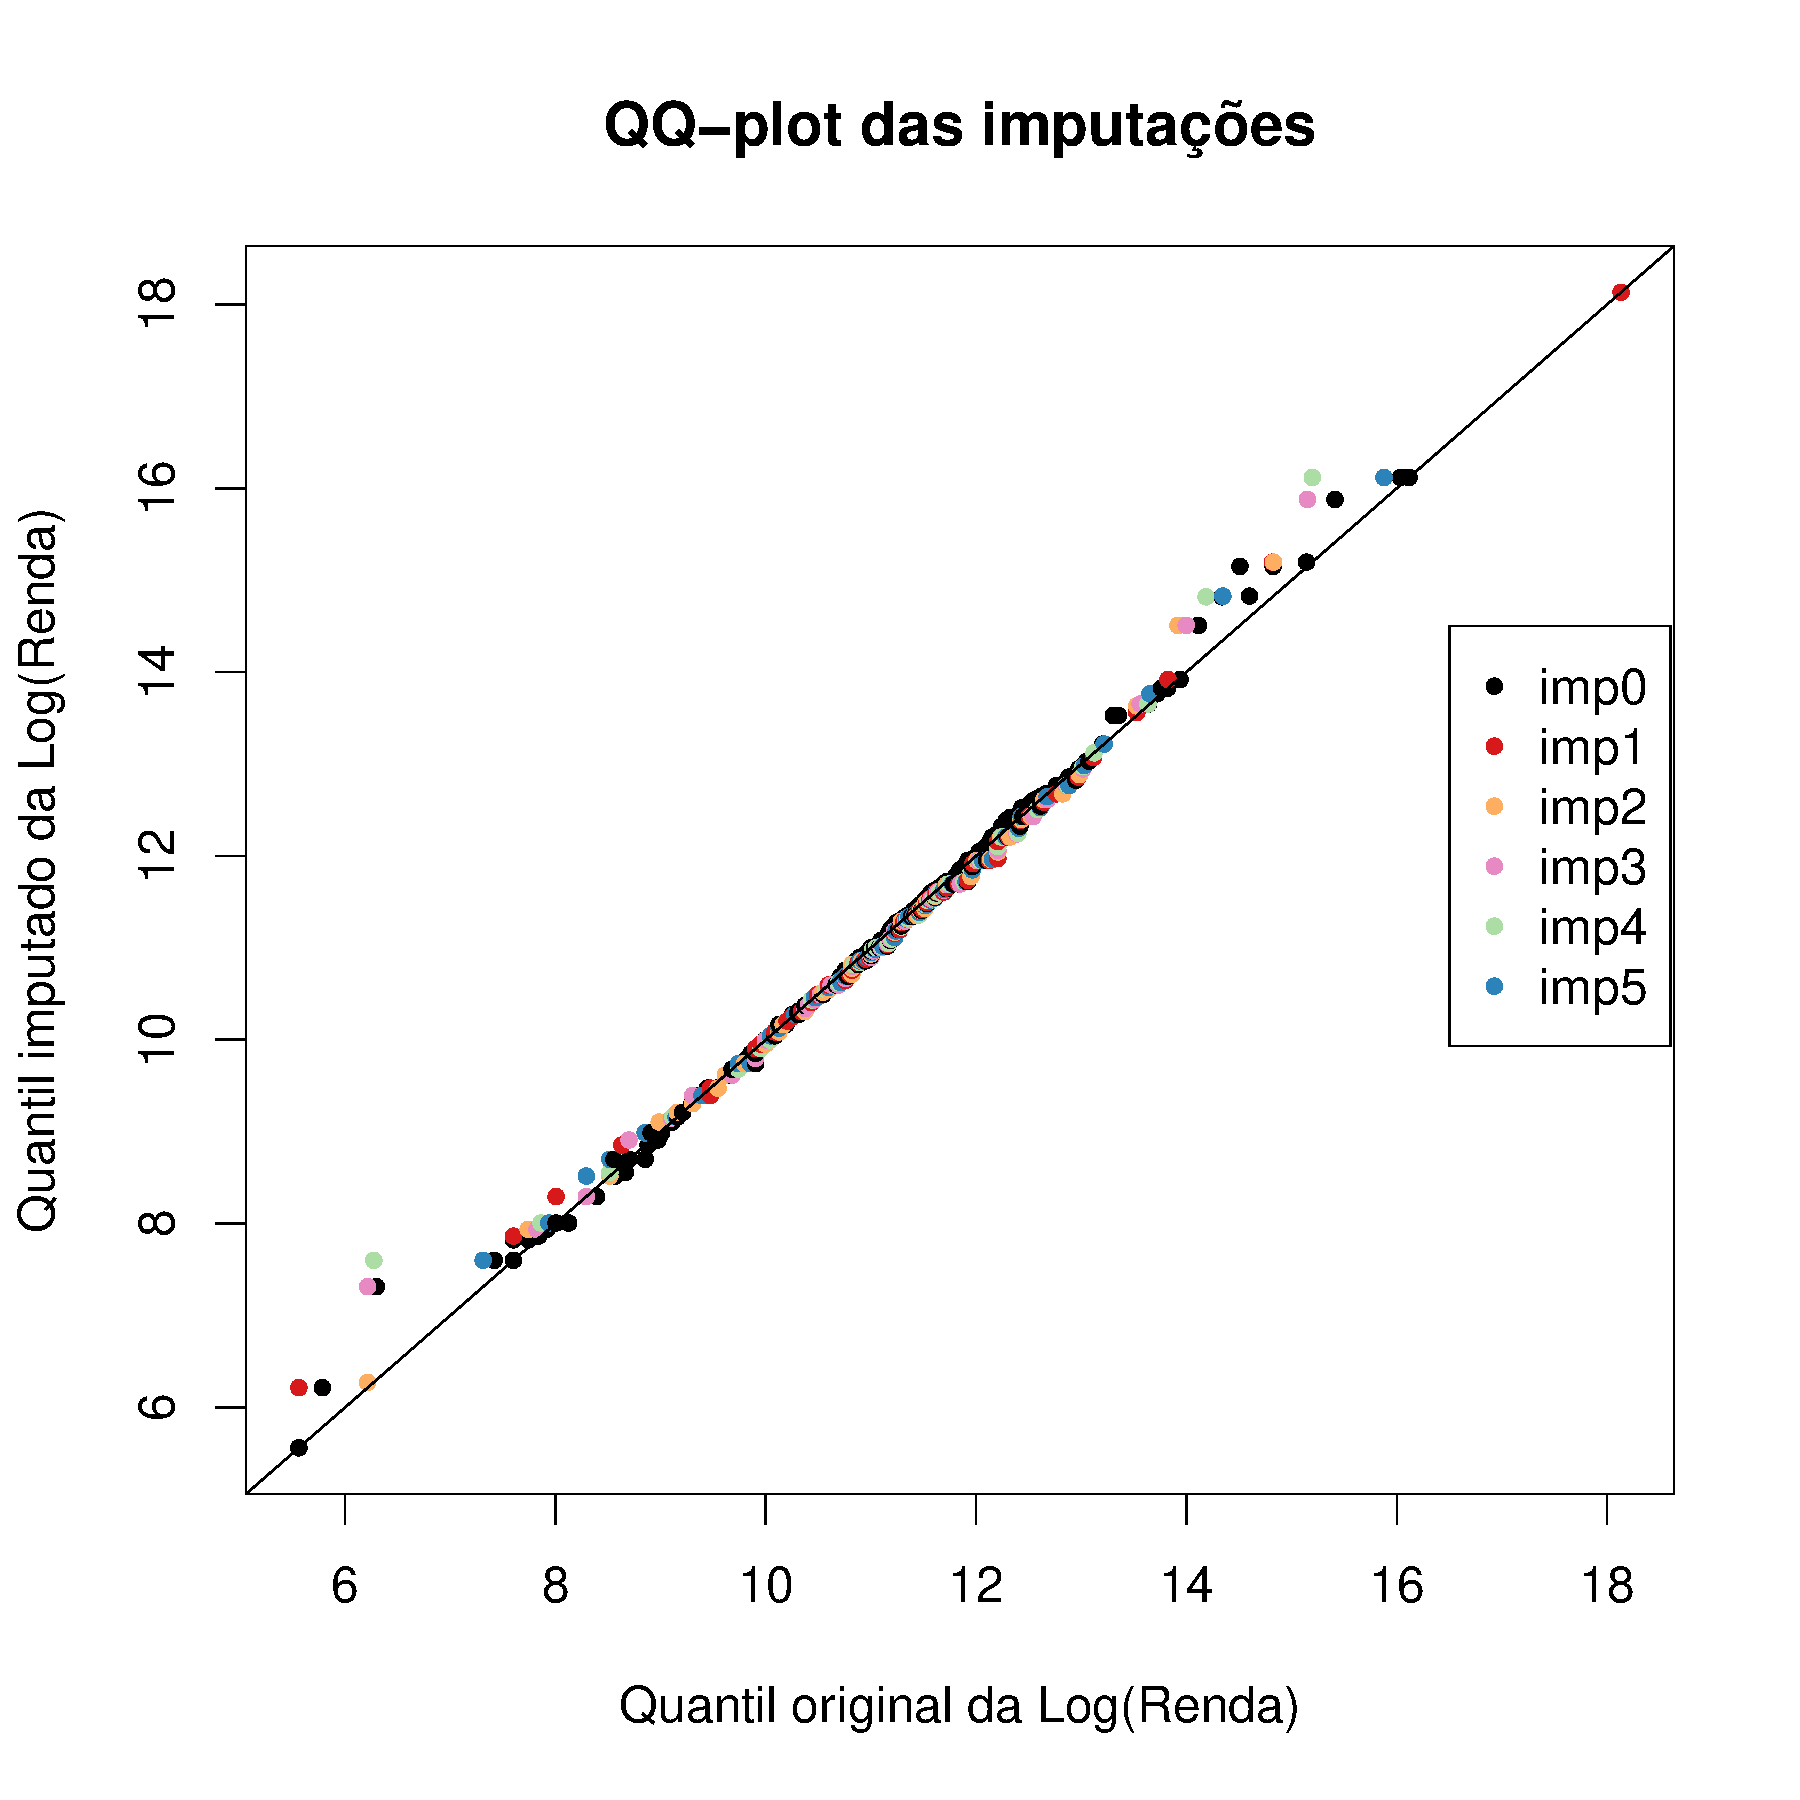
\includegraphics[width=0.6\linewidth]{p48-graf} 

}

\caption{QQ-plot das imputações, quantil imputado da Log(Renda) pelo quantil observado da Log(Renda).}\label{fig:unnamed-chunk-25}
\end{figure}

Pela Figura 17 percebemos que, para valores menores que o log(renda) de
10 e maiores que o log(renda) de 14, há um deslocamento maior entre as
imputações e a reta de adequação do modelo entre os quantis originais e
o quantis imputados da log(renda).

\paragraph{Tipo de Ensino}\label{tipo-de-ensino}

Para gerar os dados ausentes na renda, pelo caso de PA conjuntamente com
o tipo de ensino, utilizamos uma Distribuição Bernoulli com
probabilidade de sucesso (p) de 0,05 para o ensino fundamental, 0,20
para o ensino médio e 0,40 para o ensino superior, e fixamos uma semente
ao gerar os números aleatórios. Ao final obtivemos um banco de dados com
137 observações ausentes das 500 observações existentes no banco de
dados.

Os box-plots da Figura 18 estão indicando a distribuição entre os
valores da renda com o banco de dados original, o banco de dados com os
valores faltantes e as cinco imputações realizadas:

\begin{figure}[H]

{\centering 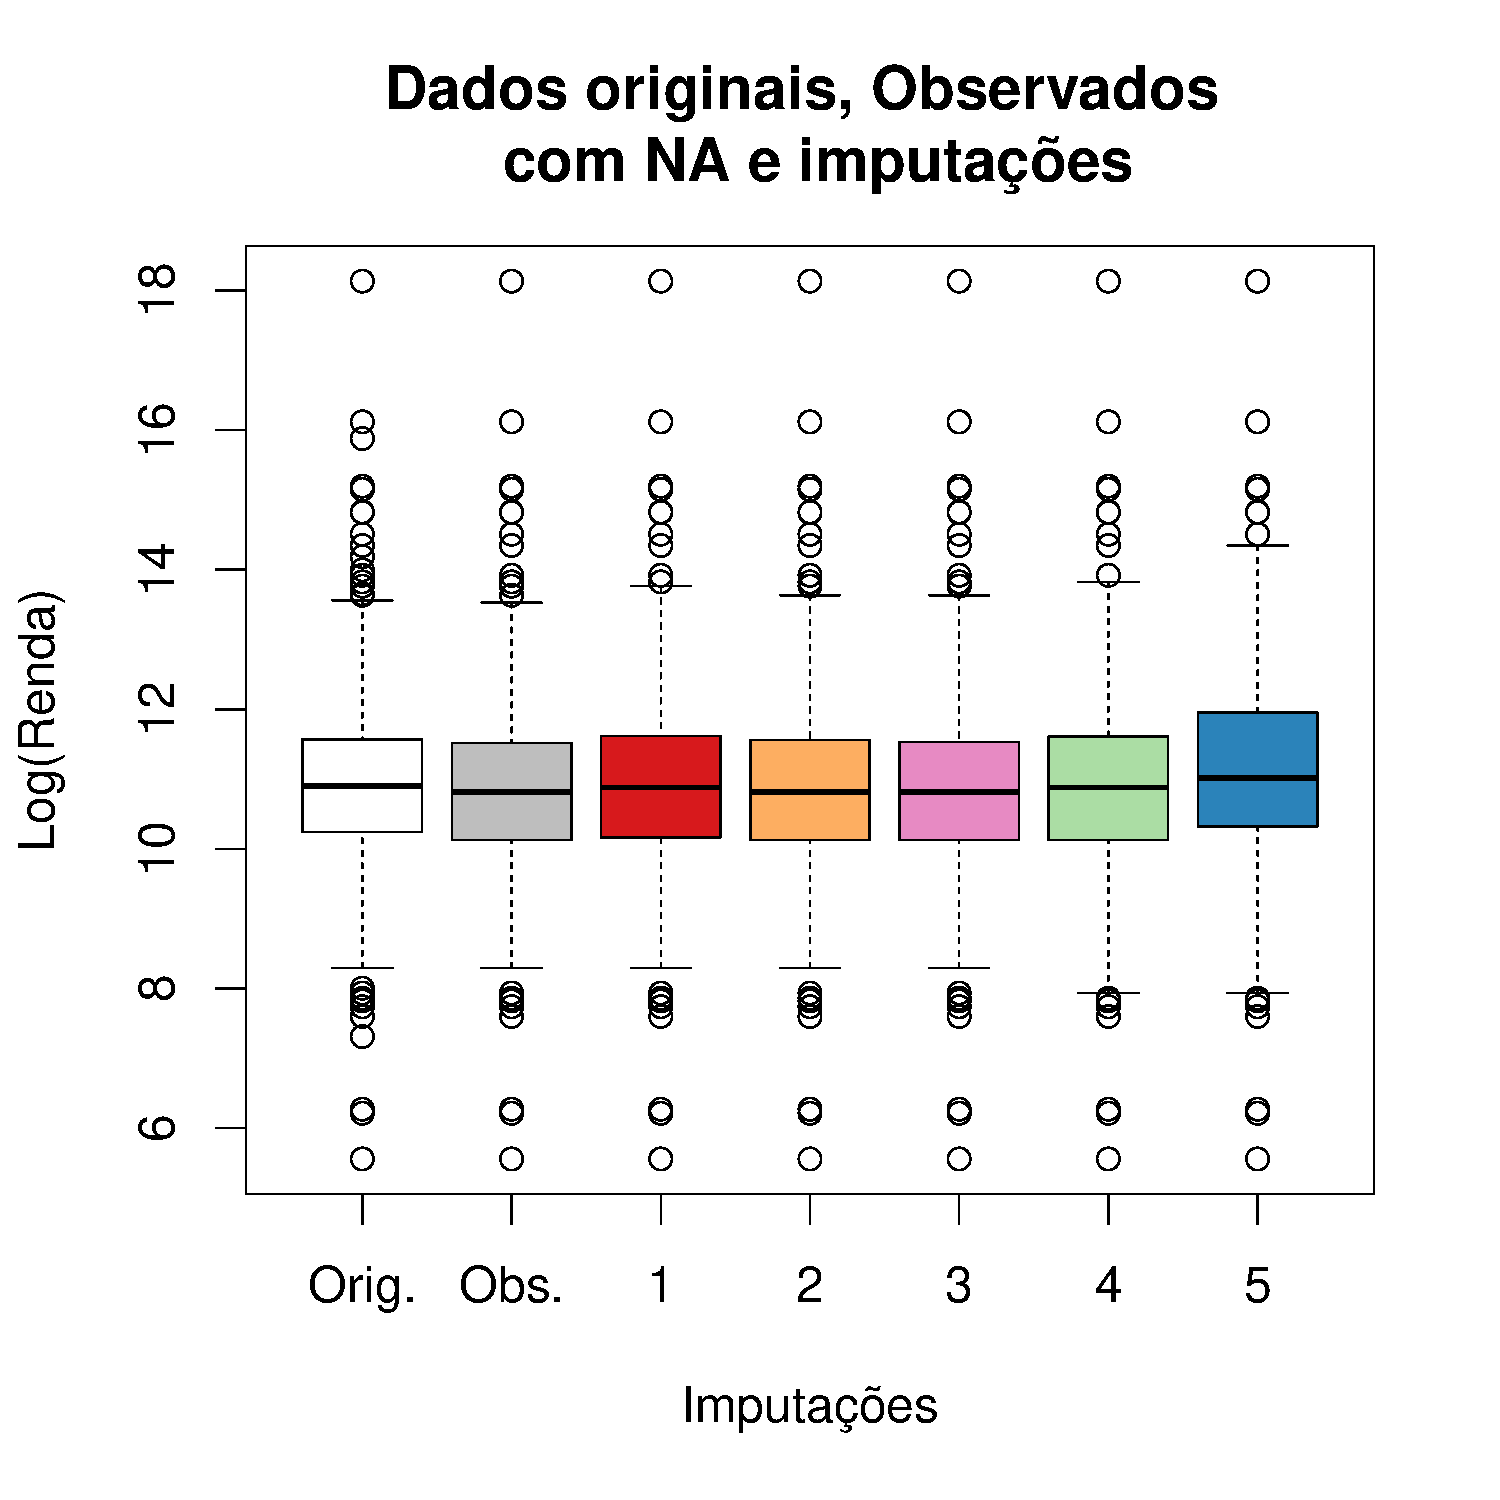
\includegraphics[width=0.6\linewidth]{p55-graf} 

}

\caption{Box-plots dos dados originais, dados observados com valores ausentes e as 5 imputações geradas.}\label{fig:unnamed-chunk-26}
\end{figure}

Pelos box-plots podemos perceber pequenas variações, a imputação nº 5
que apresentou maior divergência comparada com os outros box-plots, e
também confirmamos a variação maior encontrada na imputação nº 5, quando
esta é comparada com os dados originais da renda.

Como temos o banco de dados com os valores originais da renda, a Figura
19 demonstra a distribuição dos pontos para os dados originais e os
imputados da renda:

\begin{figure}[H]

{\centering 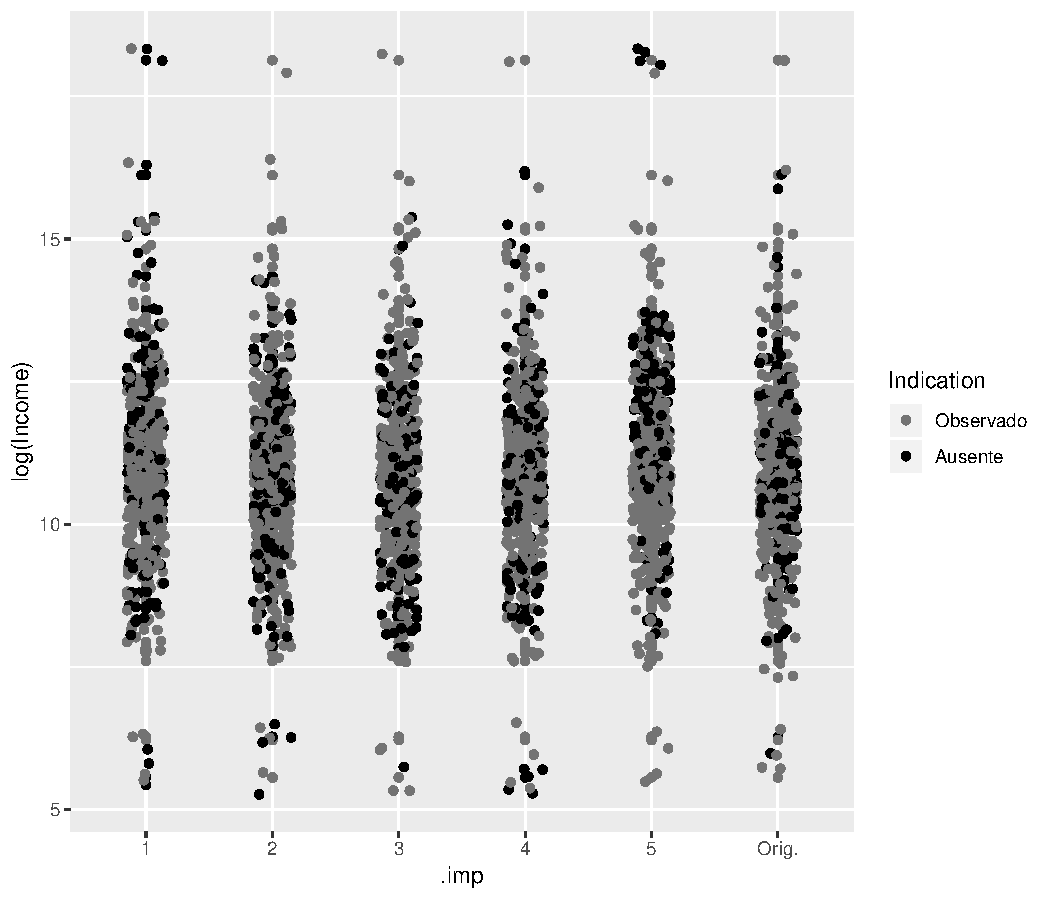
\includegraphics[width=0.6\linewidth]{Relatorio_IC_files/figure-latex/unnamed-chunk-27-1} 

}

\caption{Distribuição da Log(Renda) pelos dados originais e as imputações, as observações foram decompostas em observações originais e ausentes imputadas.}\label{fig:unnamed-chunk-27}
\end{figure}

Para analisar as variações mencionadas anteriormente, pelo gráfico de
dispersão percebemos que a imputação nº 5 não possui valores imputados
para rendas menores, sendo que a original possui valores pequenos de
renda, e as outras 4 imputações obtiveram valores imputados para rendas
ao redor do valor da log(renda) igual a 5. Percebemos também que somente
as imputações de nº 1 e 5 possuem valores altos de renda imputados. É
interessante observar o comportamento da imputação de nº 5, dado que não
segue exatamente a distribuição das outras imputações, uma vez que não
houve imputação de valores para log(renda) ao redor de 5 e houveram
imputações para log(renda) ao redor de 15.

\begin{figure}[H]

{\centering 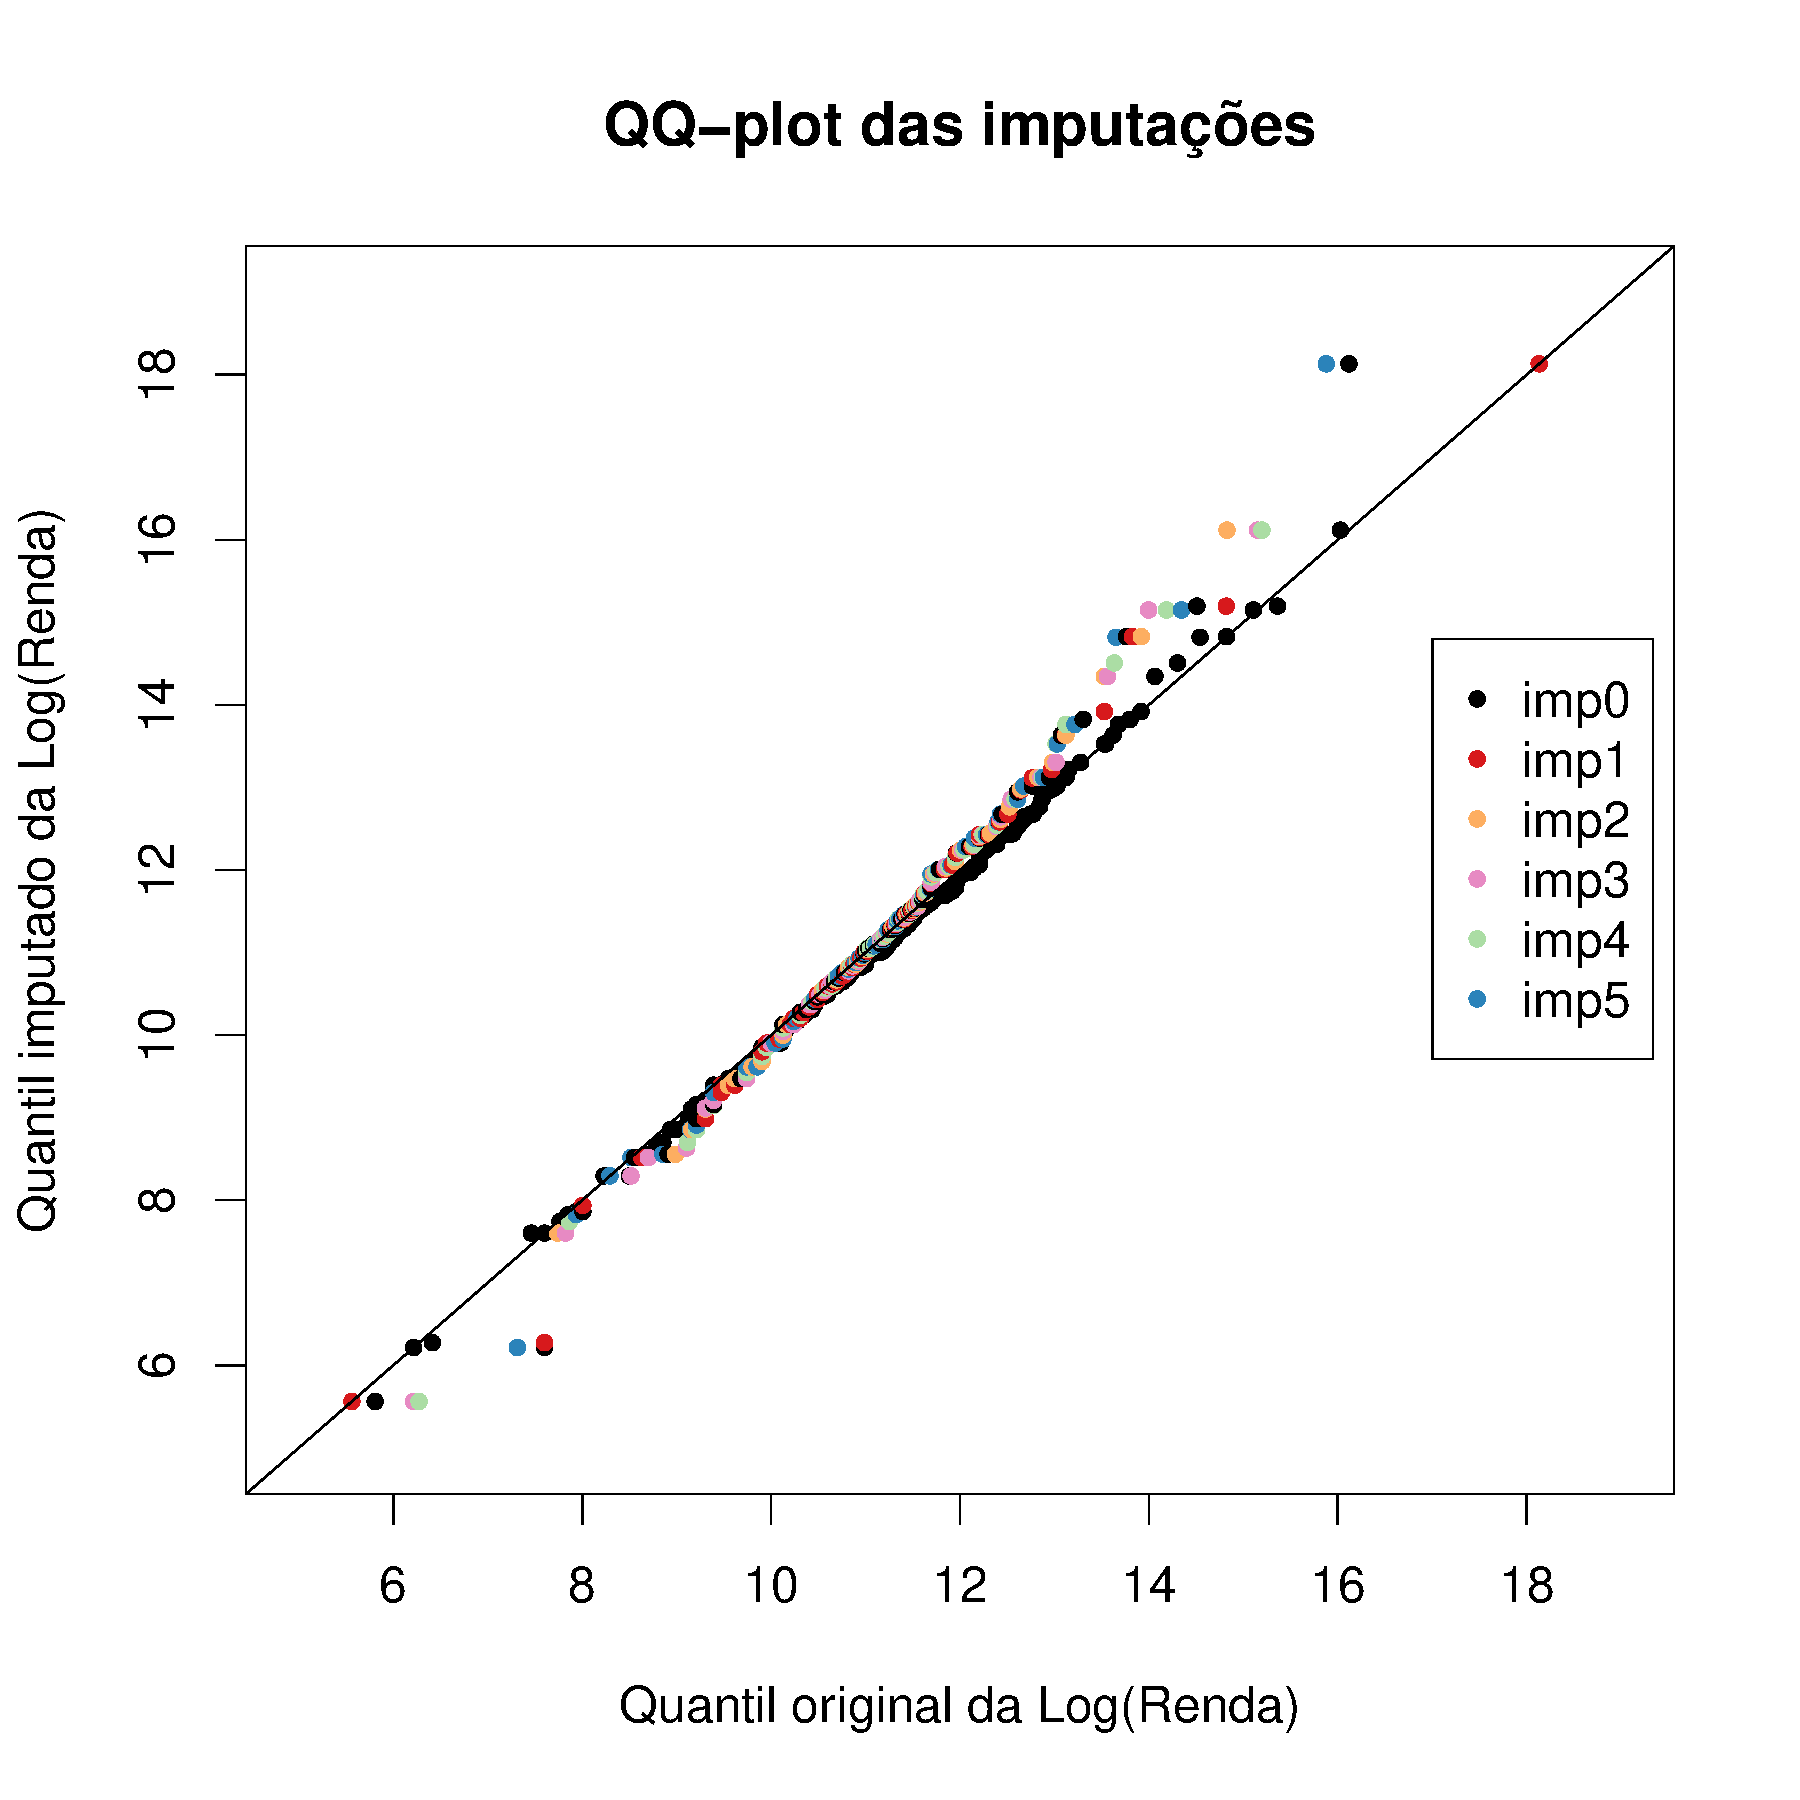
\includegraphics[width=0.6\linewidth]{p53-graf} 

}

\caption{QQ-plot das imputações, quantil imputado da Log(Renda) pelo quantil observado da Log(Renda).}\label{fig:unnamed-chunk-28}
\end{figure}

O intuito principal da Figura 20 é checar a adequação da distribuição.
Por ela percebemos deslocamentos do ajuste da reta para valores de
log(renda) menores que 8 e acima de 13, indicando que as variações
encontradas estão interferindo na adequação do modelo.

\subsubsection{Perda Não Aleatória (PNA)}\label{perda-nao-aleatoria-pna}

Para gerar os dados ausentes do mecanismo de \emph{PNA} avaliamos a
perda da variável Renda através da função logit:
\[logit(p) = log( \frac{p}{1-p} ) = log(p) - log(1-p)\]

Primeiramente retiramos uma observação constatada como um outlier,
devido a sua presença influenciar muito as medidas, assim obtemos um
banco de dados com 499 observações. Para realizar o mecanismo de PNA
nessas observações utilizamos o valor do máximo da log(renda), com
probabilidade de sucesso (p) de 0,9 e o valor da média da log(renda),
com probabilidade de sucesso (p) de 0,3. O objetivo são as
probabilidades de observações ausentes estarem ligadas a renda, ou seja,
valores de renda maiores possuem mais observações ausentes, e valores de
renda menores possuem menos observações ausentes. Assim solucionamos o
sistema de equações e encontramos os \(\beta\)'s conforme as equações
abaixo:

\[ \hat{\beta_1} = \frac{log( \frac{0,9}{1-0,9} ) - log( \frac{0,3}{1-0,3} )}{máximo - média} \]

\[ \hat{\beta_0} = log( \frac{0,9}{1-0,9} ) - \hat{\beta_1}*máximo \]

Após encontrar os \(\beta\)'s, aplicamos nos dados da renda a função
\emph{inv.logit} do pacote \emph{boot} para gerar as probabilidades de
valores ausentes em cada uma das observações, com um fixador de sementes
para a aleatoriedade das probabilidades geradas. Ao final obtivemos um
banco de dados com 144 observações ausentes das 500 observações
presentes no banco de dados.

Os box-plots da renda com o banco de dados original, o banco de dados
com os valores ausentes e as cinco imputações realizadas podem ser
vistos na Figura 21:

\begin{figure}[H]

{\centering 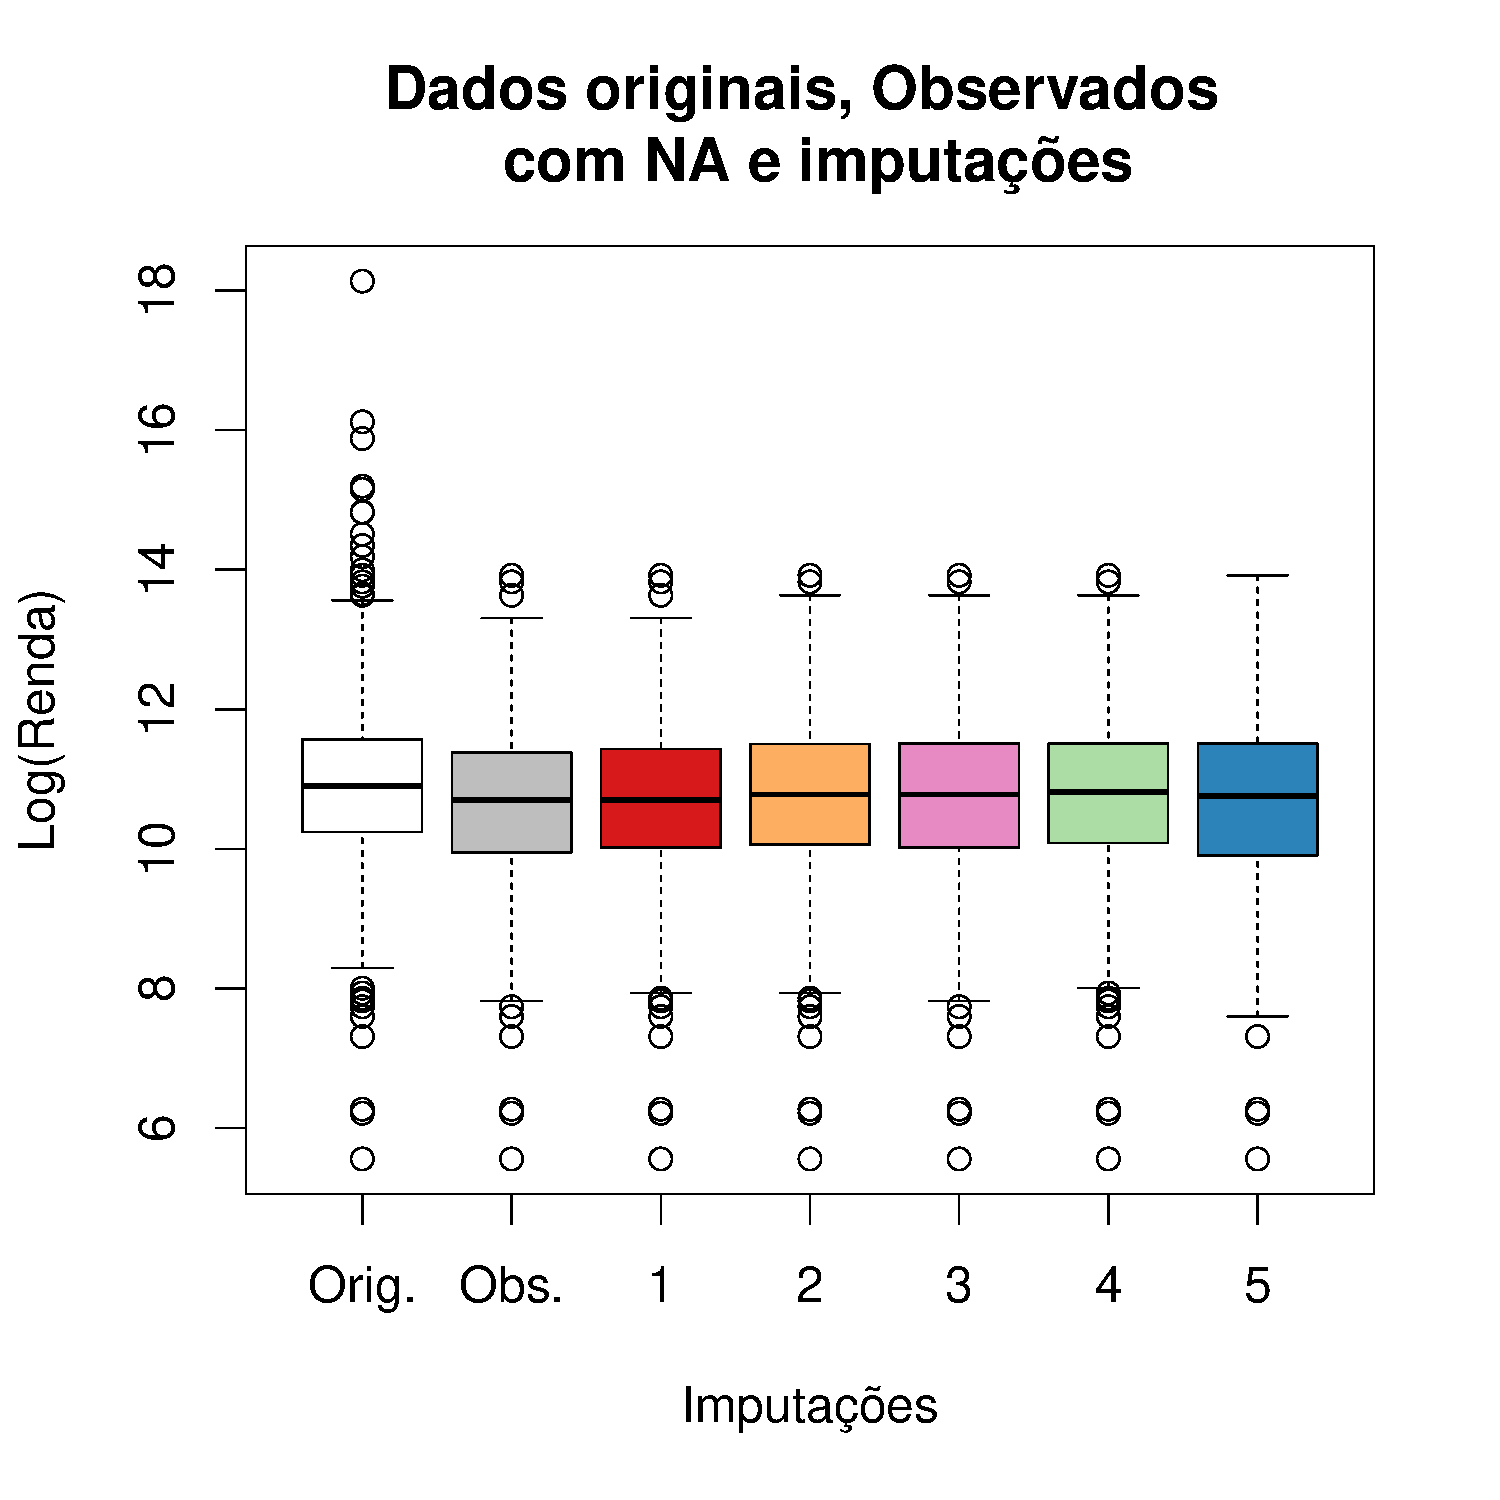
\includegraphics[width=0.6\linewidth]{p64-graf} 

}

\caption{Box-plots dos dados originais, dados observados com valores ausentes e as 5 imputações geradas.}\label{fig:unnamed-chunk-29}
\end{figure}

Nos box-plots há indícios de variações entre o banco de dados original e
as imputações. Portanto, temos a Figura 22 para verificar a distribuição
dos valores originais da renda, destacando os valores que foram
codificados como ausentes, e os valores imputados da renda:

\begin{figure}[H]

{\centering 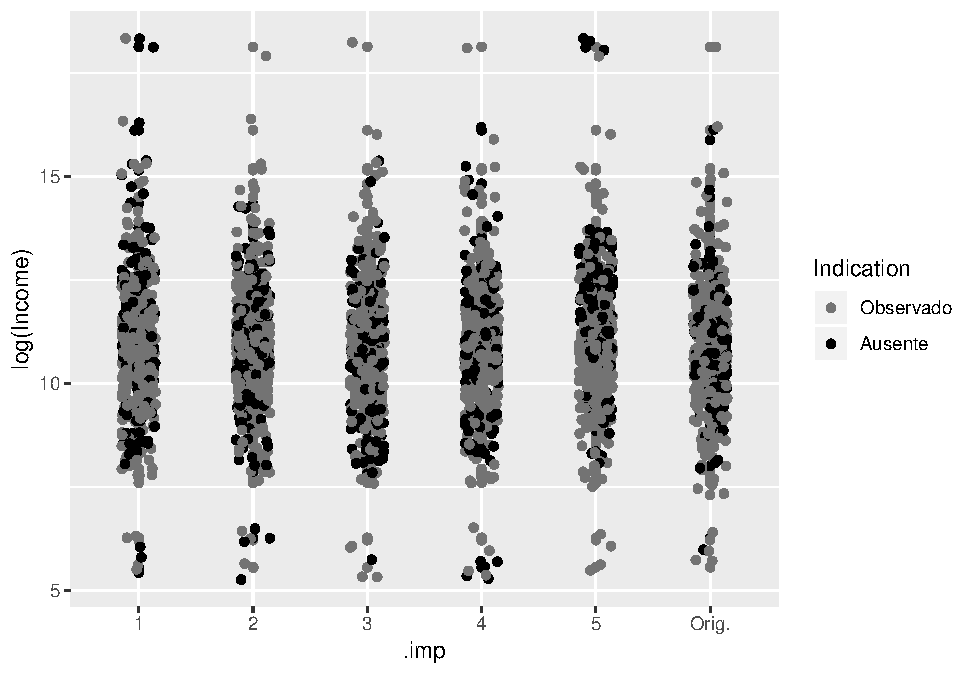
\includegraphics[width=0.6\linewidth]{Relatorio_IC_files/figure-latex/unnamed-chunk-30-1} 

}

\caption{Distribuição da Log(Renda) pelos dados originais e as imputações, as observações foram decompostas em observações originais e ausentes imputadas.}\label{fig:unnamed-chunk-30}
\end{figure}

Pela Figura 22 comprovamos alguns indícios de variações, temos que os
dados originais não possuem codificação de dados ausentes para
log(renda) ao redor de 5, e as imputações obtiveram valores imputados
próximos desse valor. Vemos também que nas imputações a partir de
aproximadamente log(renda) igual a 14 não há mais imputações, sendo que
nos dados originais percebemos codificação de variável ausente acima
desse valor de renda. Assim percebemos distribuições divergentes entre
os dados originais e os dados imputados.

\begin{figure}[H]

{\centering 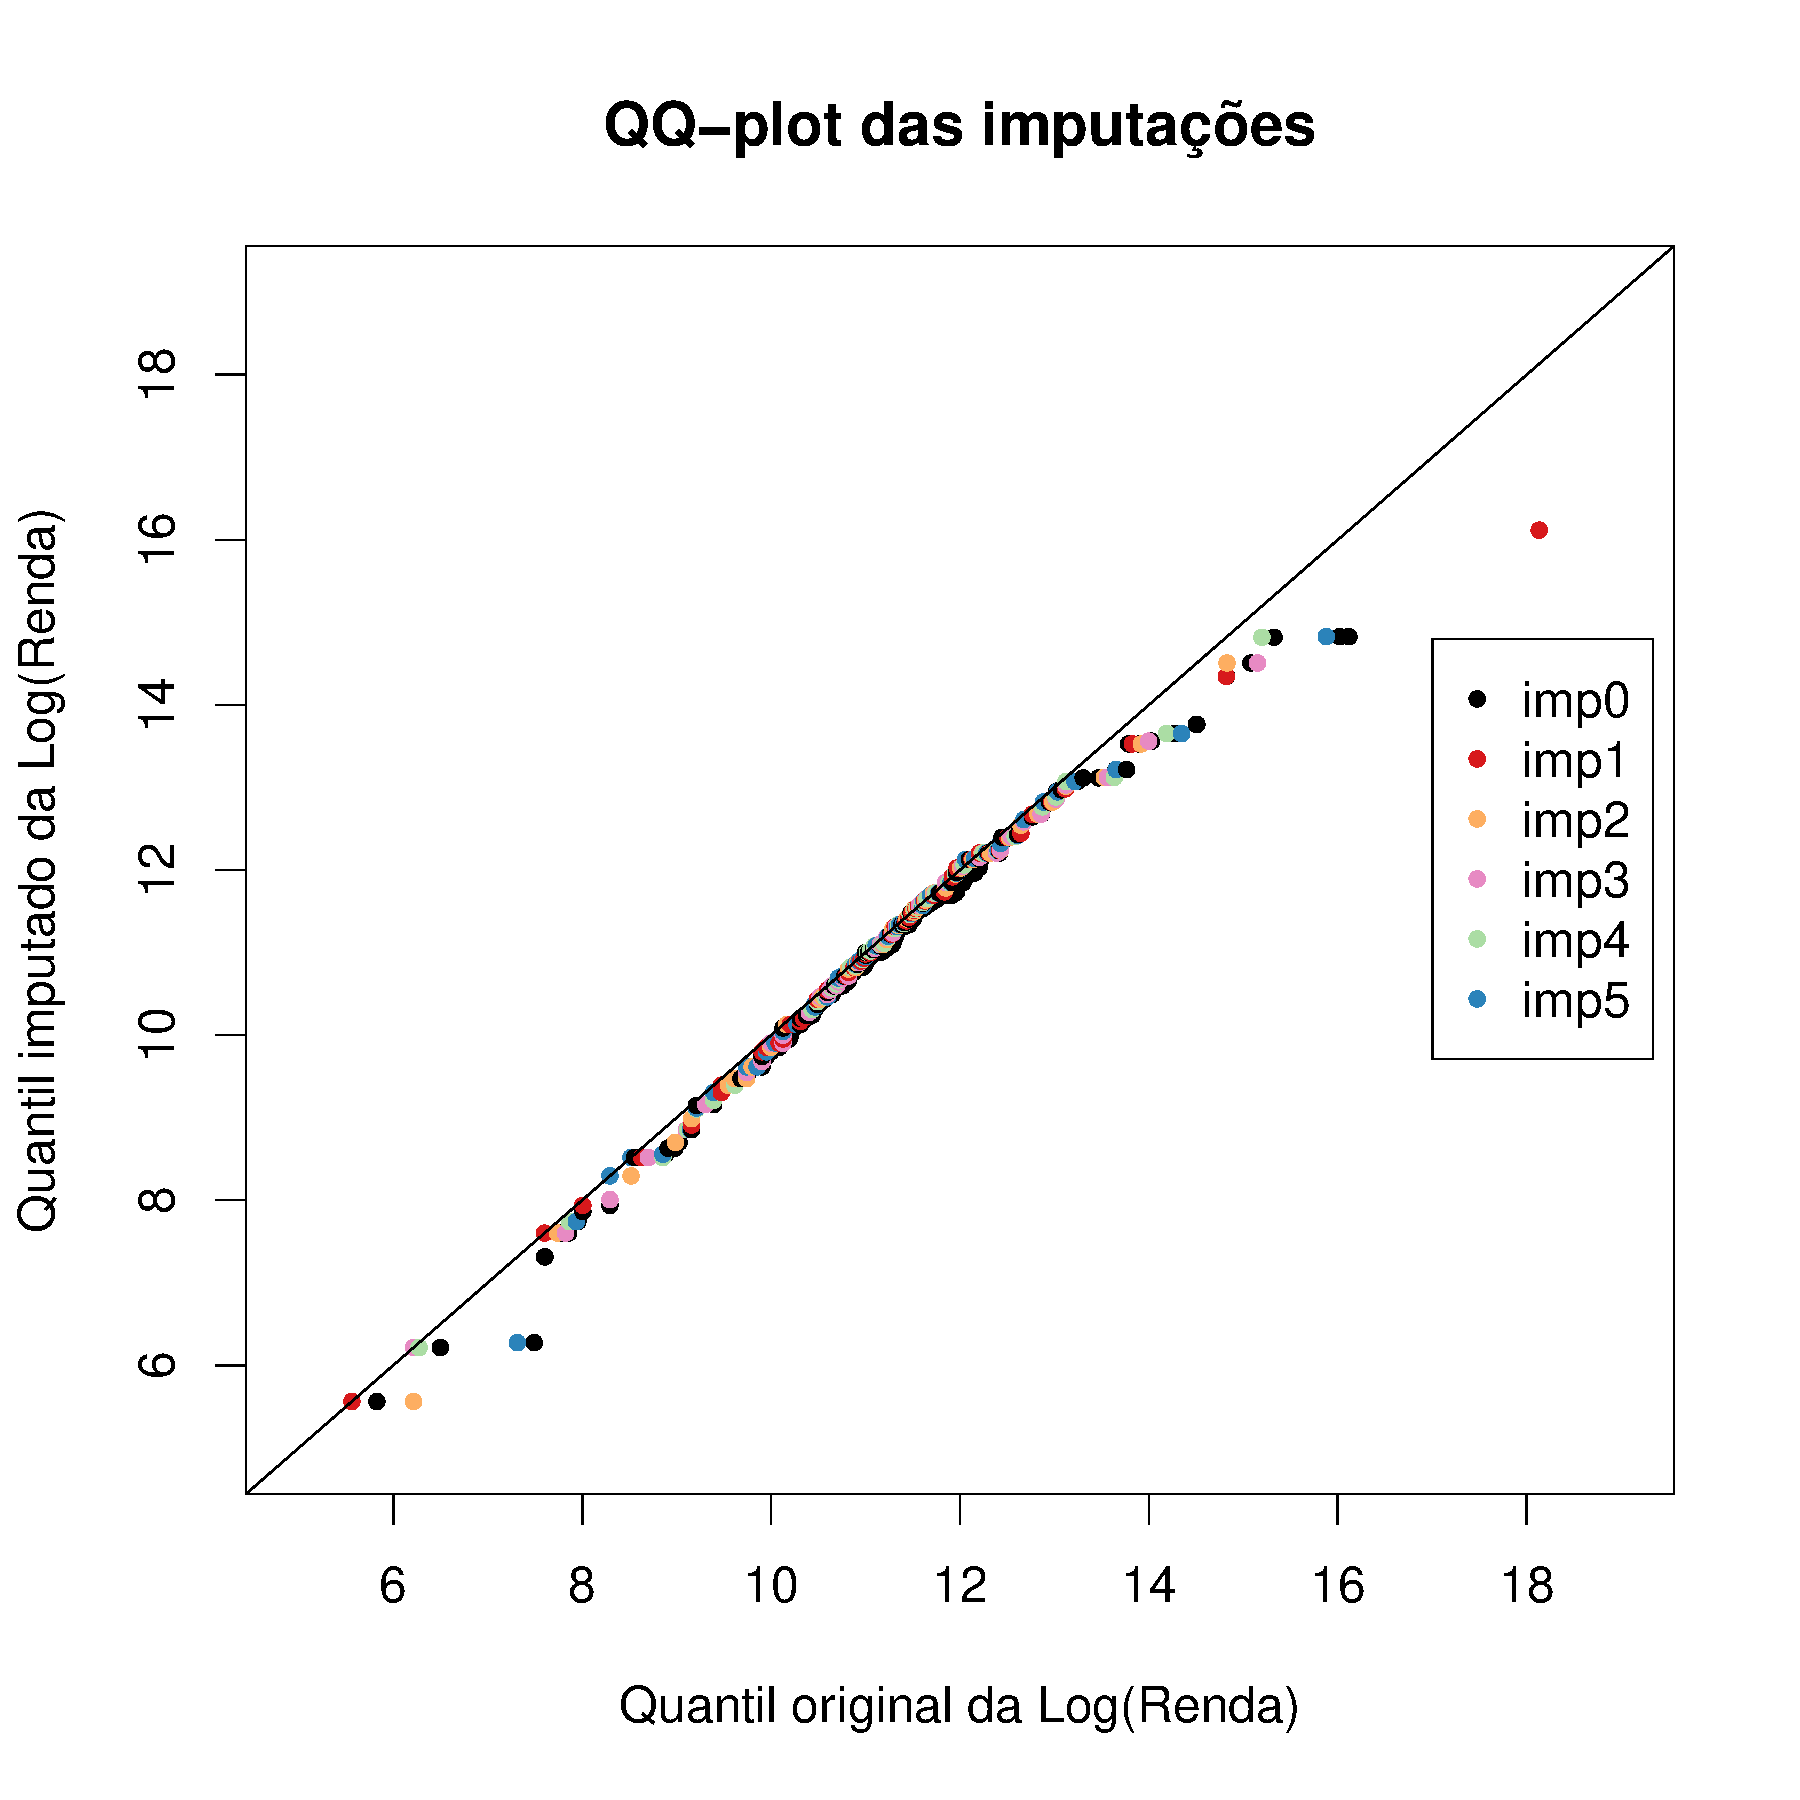
\includegraphics[width=0.6\linewidth]{p62-graf} 

}

\caption{QQ-plot das imputações, quantil imputado da Log(Renda) pelo quantil observado da Log(Renda).}\label{fig:unnamed-chunk-31}
\end{figure}

A Figura 23 indica que a adequação do modelo, entre os dados de renda
com valores ausentes e os dados de renda imputados, está demonstrando
alguns deslocamentos do ajuste da reta.

\subsection{Análise de Regressão}\label{analise-de-regressao}

Para analisar o impacto dos diferentes mecanismos de dados ausentes no
resultado de inferências feitas com os dados imputados, utilizamos o
seguinte modelo de regressão do log da renda com as demais covariáveis.

\[log(Renda)=\hat{\beta_0}+\hat{\beta_1}*x_1+\hat{\beta_2}*x_1+\hat{\beta_3}*x_3+\hat{\beta_4}*x_4+\hat{\beta_5}*x_5+\hat{\beta_6}*x_6+\hat{\beta_7}*x_7+\hat{\beta_8}*x_8+\hat{\beta_9}*x_9+\hat{\beta_{10}}*x_{10}\]

Onde \(x_1\) = Gênero Masculino, \(x_2\) = Idade, \(x_3\) = Estado Civil
(Morando Juntos), \(x_4\) = Estado Civil (Outros), \(x_5\) = Anos de
Escolaridade, \(x_6\) = Etnia Hispânico, \(x_7\) = Etnia Negro, \(x_8\)
= Etnia Outros, \(x_9\) = Ensino Médio, \(x_{10}\) = Ensino Superior; e
as bases são: Gênero Feminino, Estado Civil (Casados), Etnia Branco e
Tipo de Ensino Fundamental. De acordo com o modelo ajustado, realizamos
o cálculo dos intervalos de confiança para os mecanismos utilizando a
função do pacote \emph{mice} denominada \emph{pool}. Com isso obtivemos
a Figura 24, que contém os intervalos de confiança de 95\% dos dados
originais e dos dados das imputações dos diferentes mecanismos
analisados nessa pesquisa.

\begin{figure}[H]

{\centering 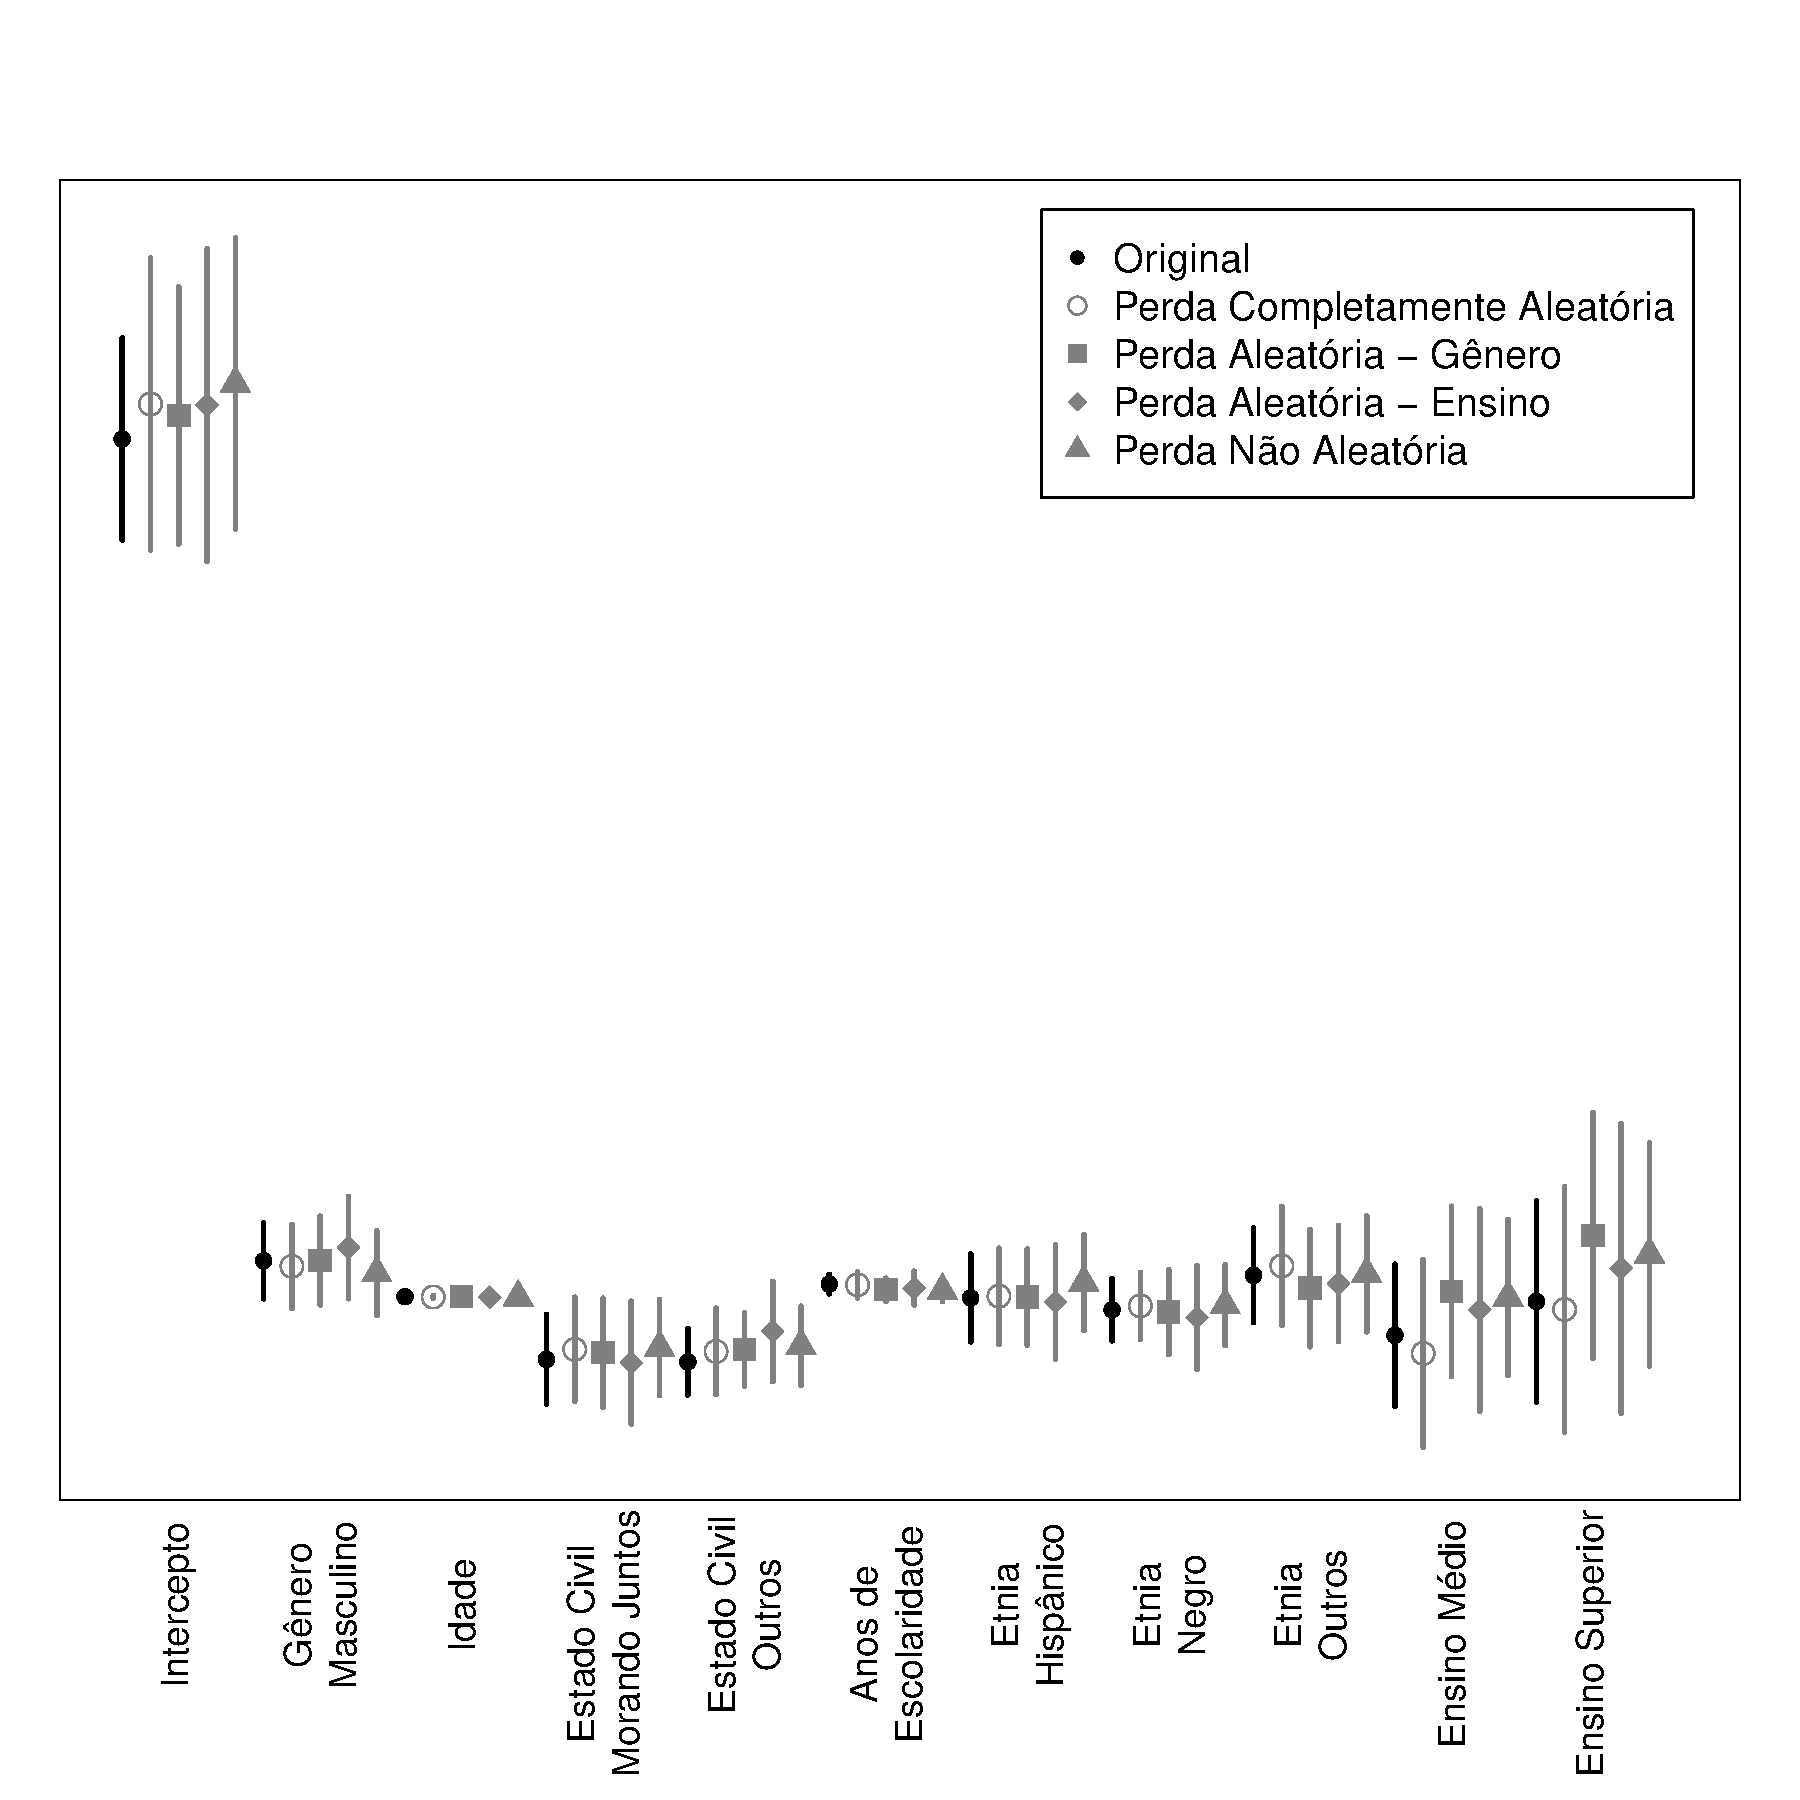
\includegraphics[width=0.6\linewidth]{reg-graf} 

}

\caption{Intervalos de confiança dos coeficientes da regressão.}\label{fig:unnamed-chunk-33}
\end{figure}

Com a Figura 24 analisamos melhor a influência de cada variável do banco
de dados no modelo ajustado. Analisando cada variável separadamente
pelos mecanismos de dados ausentes utilizados, observamos pouca
variabilidade nas variáveis Idade e Anos de Escolaridade, e muita
variabilidade no Intercepto, Ensino Médio e Ensino Superior, observando
que esses também possuem os maiores intervalos.

\section{CONCLUSÃO}\label{conclusao}

Nesse estudo analisamos o impacto dos mecanismos de dados ausentes PCA,
PA e PNA utilizando o método de Imputação Múltipla, realizando a
comparação do banco de dados original com os bancos de dados imputados
com valores ausentes.

Na seção resultados percebemos como o mecanismo influencia nas
inferências, vemos que os mecanismos de PCA e PA, por assumirem
aleatoriedade, possuem resultados próximos e o mecanismo divergente
seria o PNA, que não assume aleatoriedade. Vale ressaltar que como a
imputação foi feita assumindo a aleatoriedade da PA há uma influência
direta nas inferências dos mecanismos de PCA e PA, por isso percebemos
maiores diferenças nas inferências para os casos de PNA.

Futuramente, para medir a acurácia, seria interessante avaliar outros
métodos existentes no banco de dados utilizado nessa pesquisa e comparar
com os resultados obtidos.

Todos os códigos executados nessa pesquisa estão disponíveis em:
\url{https://github.com/fernandababarros/IC}

\section{REFERÊNCIAS BIBLIOGRÁFICAS}\label{referencias-bibliograficas}

Little, R.J.A. and Rubin, D.B. (1987). Statistical Analysis with Missing
Data. John Wiley \& Sons, New York.

Schafer, J. L. (1997). Analysis of Incomplete Multivariate Data
(Monographs on Statistics and Applied Probability). Chapman \& Hall.

Van Buuren, S., Groothuis-Oudshoorn, K. (2011). mice: Multivariate
Imputation by Chained Equations in R. Journal of Statistical Software,
45(3), 1-67. \href{http://www.jstatsoft.org/v45/i03/}{linked phrase}

Morris TP, White IR, Royston P (2015). Tuning multiple imputation by
predictive mean matching and local residual draws. BMC Med Res Methodol.
;14:75.

Frees, E.W. (2011). Regression Modeling with Actuarial and Financial
Applications, Cambridge University Press.

Van Buuren, S. (2018). Flexible Imputation of Missing Data. Second
Edition. Chapman \& Hall/CRC. Boca Raton, FL.

Camargos, V. P. et al. Imputação múltipla e análise de casos completos
em modelos de regressão logística: uma avaliação prática do impacto das
perdas em covariáveis. Cad. Saúde Pública {[}online{]}. 2011, vol.27,
n.12, pp.2299-2313.

Allison, P. D. (2001) Missing Data. Thousand Oaks, CA: Sage.


\end{document}
